%
\documentclass[12pt, oneside, reqno]{article}
\usepackage{amssymb, amsthm, amsmath,amscd, amsfonts}
\usepackage{graphics}
\usepackage[pdftex]{graphicx}
\usepackage{charter}
\usepackage{color}% http://ctan.org/pkg/color
\usepackage[linkbordercolor={1 0 1}]{hyperref}
\hypersetup{linktocpage}
\renewcommand{\ttdefault}{ptm}
\usepackage{mathpazo}
\pdfpagewidth 8.5in
\pdfpageheight 11in
\usepackage{listings}
\lstset{language=R}

%--- Page structure ---

%\addtolength{\hoffset}{-2cm}
%\addtolength{\textwidth}{4cm}
\DeclareMathOperator{\Tr}{Tr}
\renewcommand{\baselinestretch}{1.1}
\setlength{\voffset}{-.7truein}
\setlength{\textheight}{8.8truein}
\setlength{\textwidth}{6.05truein}
\setlength{\hoffset}{-.7truein}

%--------------------Environments--------------------------
\theoremstyle{definition}
\newtheorem{acknowledgement}{Acknowledgement}
\newtheorem{axiom}{Axiom}
\newtheorem{comment}{Comment}
\newtheorem{theorem}{\textbf{\textsc{Theorem}}}
\newtheorem{proposition}{\textbf{\textsc{Proposition}}}
\newtheorem{lemma}{\textbf{\textsc{Lemma}}}
\newtheorem{corollary}{\textbf{\textsc{Corollary}}}
\newtheorem{remark}{\textbf{\textsc{Remark}}}
\newtheorem{case}{Case}
\newtheorem{conclusion}{Conclusion}
\newtheorem{condition}{Condition}
\newtheorem{criterion}{Criterion}
\newtheorem{notation}{Notation}
\newtheorem{problem}{Problem}
\newtheorem{solution}{Solution}
\newtheorem{summary}{Summary}
\newtheorem{exercise}{Execrise}
\newtheorem{example}{Example}
\renewcommand{\ttdefault}{ptm}
\newtheorem*{discussion}{Discussion}
\newtheorem{definition}{\textbf{\textsc{Definition}}}

%--------------------Environments--------------------------

%---------------------Style File---------------------------
\newcommand{\R}{\mathbb{R}}
\newcommand{\U}{\mathcal{U}}
\newcommand{\OX}{\overline{x}}
\newcommand{\C}{\mathbb{C}}
\newcommand{\X}{\mathbf{X}}
\newcommand{\x}{\mathbf{x}}
\newcommand{\Z}{\mathbb{Z}}
\newcommand{\Q}{\mathbb{Q}}
\newcommand{\N}{\mathbb{N}}
\newcommand{\RR}{\mathcal{R}}
\newcommand{\OP}{\overline{\partial}}
\newcommand{\FD}{\mathfrak{D}}
\newcommand{\latex}{\LaTeX\xspace}
\newcommand{\tex}{\TeX\xspace}
\newcommand{\BTX}{{}^{b}TX}
\newcommand{\SO}{\mathcal{S}^{0,\epsilon}_{ff}}
\newcommand{\SOA}{\mathcal{S}^{0,\alpha}_{ff}}

%---------------------Style File---------------------------
\usepackage{listings}
\lstset{ %
	language=R,                     % the language of the code
	basicstyle=\footnotesize,       % the size of the fonts that are used for the code
	numbers=left,                   % where to put the line-numbers
	numberstyle=\tiny\color{gray},  % the style that is used for the line-numbers
	stepnumber=1,                   % the step between two line-numbers. If it's 1, each line
	% will be numbered
	numbersep=5pt,                  % how far the line-numbers are from the code
	backgroundcolor=\color{white},  % choose the background color. You must add \usepackage{color}
	showspaces=false,               % show spaces adding particular underscores
	showstringspaces=false,         % underline spaces within strings
	showtabs=false,                 % show tabs within strings adding particular underscores
	frame=single,                   % adds a frame around the code
	rulecolor=\color{black},        % if not set, the frame-color may be changed on line-breaks within not-black text (e.g. commens (green here))
	tabsize=2,                      % sets default tabsize to 2 spaces
	captionpos=b,                   % sets the caption-position to bottom
	breaklines=true,                % sets automatic line breaking
	breakatwhitespace=false,        % sets if automatic breaks should only happen at whitespace
	title=\lstname,                 % show the filename of files included with \lstinputlisting;
	% also try caption instead of title
	keywordstyle=\color{blue},      % keyword style
	commentstyle=\color{dkgreen},   % comment style
	stringstyle=\color{mauve},      % string literal style
	escapeinside={\%*}{*)},         % if you want to add a comment within your code
	morekeywords={*,...}            % if you want to add more keywords to the set
}
\definecolor{dkgreen}{rgb}{0,0.6,0}
\definecolor{gray}{rgb}{0.5,0.5,0.5}
\definecolor{mauve}{rgb}{0.58,0,0.82}
%-------------------------------------- redefine itemize
\def\+{+}

\makeatletter
\catcode`\ =12\let\@nl@space= \catcode`\ =10
\newcount\@nl@rlevel
\newcount\@nl@llevel
\@nl@llevel=-1

\def\@nl{%
	\catcode`\ =12
	\global\@nl@rlevel=0
	\futurelet\@nl@store\@nl@%
}
\def\@nl@gobble#1{\futurelet\@nl@store\@nl@}
\def\@nl@enditemize{
	\ifnum\the\@nl@rlevel<\the\@nl@llevel%
\end{itemize}%
\egroup%
\expandafter\@nl@enditemize%
\else%
\ifnum\the\@nl@rlevel=\the\@nl@llevel\else%
\errmessage{Error: inconsistent identation}
\fi%
\fi%
}
\def\@nl@{%
	\ifx\@nl@store\@nl@space%
	\global\advance\@nl@rlevel by 1
	\expandafter\@nl@gobble%
	\else%
	\catcode`\ =10
	\ifx\@nl@store+%
	\ifnum\the\@nl@rlevel>\the\@nl@llevel%
	\bgroup%
	\@nl@llevel=\the\@nl@rlevel
	\begin{itemize}%
		\fi%
		\@nl@enditemize%
		\item \expandafter\expandafter\expandafter\@gobble%
		\else%
		\ifx\@nl@store\@nl%
		\global\@nl@rlevel=-1\relax\@nl@enditemize\par
		\else\space\fi%
		\fi%
		\fi%
	}
	
	\catcode`\^^M=\active%
	\AtBeginDocument{%
		\catcode`\^^M=\active%
		\let^^M=\@nl%
	}%
	\catcode`\^^M=5
	\makeatother
	%------------------------------------------------
	
\begin{document}
		\begin{center}
			\medskip
			{\huge Notes for B-calculus} \\
			{\small \textbf{Scribe}: Zhou Changwei; \textbf{Lecturer}: Paul Loya}\\
			{\small \textbf{Attendant}: Kunal Sharma, Huang Binbin, Adam Weisblatt, Zhou Changwei}
		\end{center}
\begin{center}
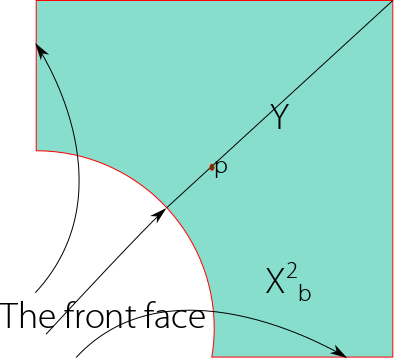
\includegraphics[width=100mm]{drawing32.png}
\end{center}
\tableofcontents
\section{Lecture 1:From AS to APS}
Let $M$ be a compact manifold without boundary. Let $D^+$ be a Dirac operator acting between sections of Hermitian vector bundles $E^+, E^-$, i.e we have
\begin{align}
D:C^{\infty}(M,E^+)\rightarrow C^{\infty}(M, E^-)
\end{align}
such that the Riemannian metric is given by the principal symbol of $D^{+}D^{-}$:
\begin{align}
\sigma(D^{+}D^{-})(\xi)=|\xi|^{2}
\end{align}
We know that if we let
$$D=
\begin{bmatrix}
0 & D^+\\
D^- & 0
\end{bmatrix}
$$
Then the above can be translated to
\begin{align}
D: C^{\infty}(M, E^{+}\oplus E^{-})\rightarrow C^{\infty}(M, E^{-}\oplus E^{+})
\end{align}
The core fact we need is $D$ is elliptic.

Let us recall the proof of Atiyah-Singer index theorem we proved last year. The essential argument is the \textbf{Fedosov's formula}: To review the set up, we let
\begin{align}
B(t)=D^{-}\int^{t}_{0}e^{-sD^+D^-}ds
\end{align}
Then formally we have
\begin{align}
D^+B&=D^+D^-\int^{t}_{0}e^{-sD^+D^-}ds\\
&=\int^{t}_{0}D^+D^- e^{-sD^+D^-}ds\\
&=-\int^t_0 \partial_s e^{-s D^+D^-}ds\\
&=Id-e^{-tD^+D^-}
\end{align}
Therefore we conclude that
\begin{align}
BD=Id-e^{-tD^+D^-}, DB=Id-e^{-tD^+D^-}
\end{align}
Further we have
\begin{align}
e^{-tD^+D^-}, e^{-tD^+D^-}\in \Psi^{-\infty}
\end{align}
and they are both Hilbert-Schmidt operators. In particular they are both trace class. We now conclude:
\lemma{Fedosov's formula}:
As long as $D$ is Fredholm so that $Ind D$ is well defined, we have
\begin{align}
Ind D=\lim_{t\rightarrow 0}Tr(e^{-tD^-D^+})-Tr(e^{-tD^+D^-})
\end{align}
because the value on the right hand side is in fact independent from $t$.  Now taking the limit and after some work by Getzler, we have:

\theorem{Atiyah-Singer}:
\begin{align}
Ind D={\frac{1}{(4\pi i)^{m}}\int_{M}(\det)^{1/2}(\frac{\mathcal{R}/2}{\sinh(\mathcal{R}/2)})Tr(\tilde{Z}e^{\tilde{Q}})}
\end{align}
\noindent
Now our goal is to generalize to manifolds with boundary:
\begin{center}
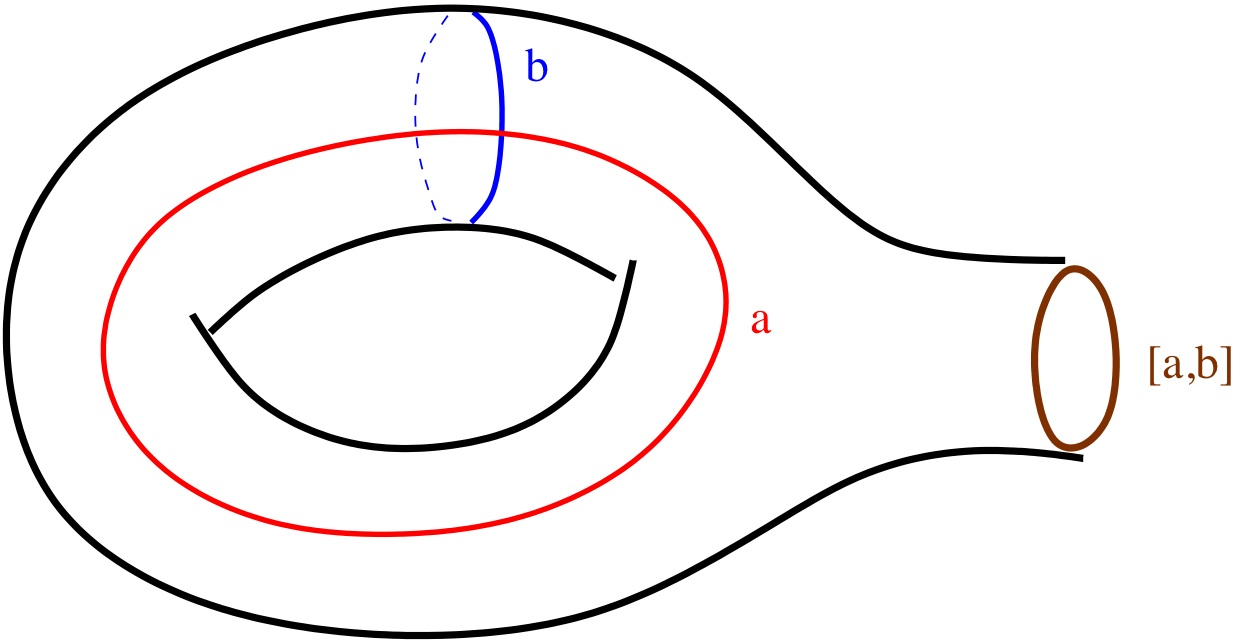
\includegraphics[width=180mm]{Lecture11.jpg}
\end{center}
\example Collar boundary:
For simplicity we assume the following scenario: Let $M=[0,1]\times Y$, and $Y$ is a closed manifold. The collar is then of the form $[0,1)_{x}\times Y$. Now assume we have an Hermitian vector bundle $E^\pm$ over $M$ with an associated Dirac operator
$$
D^+:C^{\infty}(M,E^+)\rightarrow C^{\infty}(M,E^-)
$$
such that
+
$D$ is ellipitic.
+
Over the collar part we have
$$
D=\frac{1}{i}\sigma(\partial_{X}+D_{y})
$$

Here $\sigma: E^{+}\rightarrow E^{-}$ is a fibre-wise bundle isomorphism given by the principal symbol. In other words:
$$
\sigma=\sigma(D)(i\partial_{X})
$$
and we let $D_{y}=A$ be a first order differential operator:
$$
A: C^{\infty}(Y_0, E^+)\rightarrow C^{\infty}(Y_0, E^-)
$$
Now to be simple if we let
$$
g=dx^{2}+g_{y}
$$
to be the product metric, then the fact that
$$
\sigma(D^+D^-)=g^{2}
$$
is equivalent to $\sigma^{*}\sigma=Id$. To be more precise we have:
\begin{align}
\sigma(\sigma^{*}\frac{1}{i}\partial_X+A^{*})(\sigma\frac{1}{i}\partial_{X}+A)=g^{2}
\end{align}
Expanding out we have
\begin{align}
\sigma*\sigma^{*}=Id, \sigma^{*}A+A^{*}\sigma=0, \sigma_{Y}(A^{*}A)=g_{y}
\end{align}
These are the conditions we are going to use afterwards.
\example
Let
$$
M=S^{1}\times [0,1], \tilde{M}=S^{1}\times \R, Y=C^{*}=\mathbb{S}^{1},g_{M}=dx^{2}+\theta^{2}
$$
Now we let
$$
D^+=\frac{1}{i}(\partial_{x}+i\partial_{\theta}), F_{k}(x,\theta)=e^{k(x+i\theta)}
$$
Then we have
$$
D^-D^+=\partial_{x}^{2}+\partial_{\theta}^{2}, D^-D^+(F_k(x,\theta))=0
$$
It now turns out that $D^-D^+F_{k}(x,\theta)=0$ for all $k\in \R/2\pi\mathbb{Z}\cong \mathbb{S}, k\not=0$.  So $\dim(\ker)$ is uncountable. Thus $D^-D^+$ (and $D^+$ itself) is no longer Fredholm.

\discussion
So it is clear that we  no longer have Fredholm condition on the boundary. The main issue is the bad behavior near the boundary part of the manifold. To fix this by killing off the extra spaces in the kernel of $D$, we have two approaches.
+
The first choice is to impose suitable boundary conditions.
+
The second choice is to limit our function space by working with special function spaces, like $H^{s}$ Soblev spaces.
+
The idea of the Atiyah-Singer-Patodi(APS) paper is as follows: Let us take a cyclinderal end
$$
(-\infty, 0]\times Y
$$
where $Y$ is the boundary part of $M$, and glue it with $M$ to form a manifold with cylinderal end:
$$
\tilde{M}=(-\infty, 0]_{x}\times Y\bigcup M
$$
Then $\tilde{M}$ is a non-compact manifold without boundary!

\example
To see why the boundary case is bad, let us consider an example and see why Fredholm property fails: Let $$D^+=\frac{1}{i}\partial_{x}, \tilde{M}=\R, M=[0,1], \tilde{D}=\frac{1}{i}\partial_{x}, M\cong [0,1]\times Y_0, Y_0=\{*\}$$
Now use integration by parts we have
\begin{align}
D^-=-D^{+}, D^-D^+=-\partial_{x}^{2}
\end{align}
Thus we have
\begin{align}
e^{-tD^-D^+}\phi(x)=\int_{x'\in \R}\frac{1}{\sqrt{4\pi t}}e^{-\frac{(x-x')^{2}}{4t}}\phi(x')dx'
\end{align}
Now the trace of a Hilbert-Schmidt operator by definition is given by integral over the kernel $x=x'$:
\begin{align}
Tr(e^{-tD^-D^+})=\int_{x,x'\in \R}\frac{1}{\sqrt{4\pi t}}dx=\infty, \forall t>0
\end{align}
Therefore the Fedosov formula does not even hold for a one dimensional case when the boundary is a point!

\example
In general, the Fedosov's formula fails because the heat kernel is not integrable at the diagonal:  We can write the heat-kernel as
\begin{align}
e^{-tD^-D^+}|_{(-\infty, \epsilon)|_{x}\times Y}=\frac{1}{\sqrt{4\pi t}}e^{-\frac{(x-x')^{2}}{4t}}*e^{tD_{y}^{2}}+A
\end{align}
where $A$ is some operator in trace class. This is because we can write
\begin{align}
D^+=\frac{1}{i}\sigma(\partial_{x}+D_{y}), D^{-}D^{+}=-\partial_{x}^{2}+D_{y}^{2}
\end{align}
Therefore formally we have
\begin{align}
e^{-tD^-D^+}=e^{-t\Delta_\R}*e^{tD_{y}^2}+A
\end{align}
and after integration the same singularity would occur on the $x$-axis:
\begin{align}
Tr(e^{-tD^-D^+})&=A+\int \frac{1}{\sqrt{4\pi t}} e^{-\frac{(x-x')^{2}}{4t}}e^{-tD_{y}^{2}}dy\\
&=\infty*Tr(e^{-t D_{y}^{2}})\\
&=\infty
\end{align}
So Fedosov's formula fails if we do not introduce some regularization procedure.

\remark
Prof. Loya pointed out we get from line (18) to line (19) because the heat kernel is defined everywhere on $M$, and in particular away from the cylinder.
\discussion
To resolve this, let us consider
\begin{align}
D=\frac{1}{i}\partial_{X}+A
\end{align}
where $A$ is invertible on the cylinderal end. And assume that there exists $\tilde{D}$ such that $D$ is the restriction of $\tilde{D}$.  Now consider the space of functions:
\begin{align}
u\in C^{\infty}(M,E^+)\cap L^{2}(M, E^+), Du\in L^{2}(M,E^+)
\end{align}
In this case $\tilde{D}$ is Fredholm and we can compute its index as before. However if we do like we did earlier, then we realize $DB=I-K_1$, and $K_1$ is no longer trace class. Thus the trace does not even exist!

\remark
Prof. Loya suggested we restored Fredholm property because $L^{2}$ spaces.

\discussion
Thus the issue is that $e^{-tD^-D^+}\not\rightarrow 0$ as $x\rightarrow -\infty$.  This is why when we integrate on the $x$-axis we get $\infty$.

To resolve this issue Melrose introduced the following operator $E$:
 \begin{align}
E&=\int_{\tau \in \R}e^{-(x-x')\tau} (i\tau+A)^{-1}i\sigma d\tau\\
&=p(x)p(x')\int e^{-(x'-x)\tau}(i\tau+A)^{-1}i\sigma d\tau
 \end{align}
 Here $p: \R\rightarrow \R$ is a smooth cut-off function that is 1 on $(-\infty, \epsilon)$. The idea of $E$ is that it is a partial inverse of $\tilde{D}$. Let us compute on the cylinder part of $M$:
 \begin{align}
 \tilde{D}Eu(x)&=\frac{1}{i}\sigma(\partial_{x}+A)\circ Eu\\
 &=\frac{1}{i}\sigma(\partial_x+A)p(x)\int e^{ix\tau}(i\tau+A)^{-1}i\sigma \tilde{u}(\tau)d\tau\\
 &=\frac{1}{i}\sigma(\int_{\R}e^{ix\tau}(i\tau+A))(i\tau+A)^{-1}\tilde{u}(\tau)d\tau)\\
 &=\frac{1}{i}\sigma\int_{\R} e^{ix\cdot \tau}\tilde{u}(\tau)d\tau\\
 &\approx u(x)
 \end{align}
 \remark It is unclear how we get from (31) to (32) with the extra $\frac{\sigma}{i}$.
\discussion Therefore we should have
 $$
 \tilde{D}E\approx Id+\textrm{Nice Term}
 $$
 This is the motivation behind $B$-calculus. We now consider
 \begin{align}
 B'=B+Ee^{-tD^+D^-}
 \end{align}
 Now  we no longer distinguish $D$ and $\tilde{D}$, the reader should be able to tell:
 \begin{align}
\tilde{D}B'&=\tilde{D}B+\tilde{D}Ee^{-tD^+D^-}\\
&=Id-e^{-tD^+D^-}+D^+Ee^{-tD^+D^-}\\
&=Id-K_1, K_1=e^{-tD^+D-}-D^+Ee^{-tD^+D-}
 \end{align}
 and analogously we may define $K_2$.  Our claim is
 \proposition
 $K_1, K_2$ are now both in trace class!
 \discussion
 So this is good news. We now recover that
 \begin{align}
 Ind D&=Tr(K_2)-Tr(K_1)\\
 &=Tr(e^{-tD^-D^+}-Ee^{-tD^-D^+}D^+)-Tr(e^{-tD^+D-}-D^+Ee^{-tD^+D-})\\
 &=(Tr(e^{-tD^-D^+})-Tr(e^{-tD^+D^-}))+Tr([D^+, Ee^{-tD^+D^-}])\\
 &=h(t)+g(t)\\
 &=\int AS+\textrm{error term}\\
 &
 =\int AS+ \lim_{t\rightarrow 0}g(t)
 \end{align}
 Now we reached the $\eta$-invariant:
\theorem:
$$
Ind D=\int AS-\frac{1}{2}\eta(0), \eta(0)=\int^{\infty}_{0}t^{-\frac{1}{2}}Tr(e^{-tD_{y}^{2}})dt, \eta(s)=\sum_{\lambda \in Spec(\Delta}\frac{sgn(\lambda_{n})}{|\lambda_{n}|^{s}},s\in \C
$$

\section{Lecture 2: The $b$-integral and $b$-trace}
This is our main object of study for this lecture:
\begin{center}

\includegraphics{Lecture21.png}
\end{center}
Let us review the set up. Let $M$ be a manifold with cylinderal end. On the end we have
$
M\cong (-\infty, 0]\times Y
$
where $Y$ is a closed manifold. Here $M$ is Riemannian and the metric over the cylinder part is given by
$
g|_{\textrm{cylinder}}=dx^{2}+g_Y
$
where $g_Y$ is the metric on $Y$. Now let $E=E^+\oplus E^-$ be an $\Z_2$ graded Hermitian vector bundle over $M$.  We have an associated Dirac operator $D^{+}: C^{\infty}(M,E^+)\rightarrow C^{\infty}(M, E-)$. Now by the discussion in Lecture 1, we assume that we have
\begin{align}
	D^+=\frac{1}{i}\sigma(\partial_{x}+A), A: C^{\infty}(Y, E^\pm_{0})\rightarrow C^{\infty}(Y, E^\pm_{0}), E^\pm_{0}=E^\pm|_{x=0}, \sigma: E^+_{0}\rightarrow E^-_{0}, \sigma\sigma^{*}=Id
\end{align}
such that $A$ is self-adjoint and $\sigma=\sigma_{D^+}(dx)$ is the bundle isomorphism given by the principal symbol of $D^+$. In the previous lecture we called $A$ by $D_{y}$. We are going to use $D_{y}$ and $A$ interchangably.
\discussion
Adam asked the question that what is the form of $D^+$ on a product manifold. For example consider $D^+=d$. Loya suggested as follows: Let $\alpha$ be a $k$-form on $M$, then $\alpha$ can be written as
\begin{align}
	\alpha=\sum_{|I|}a_{I}(x,y)dy_{I}+\sum_{|J|=k-1}b_{I}(x,y)dx\wedge dy_{|J|}=\beta_1(x,y)+dx\wedge \beta_2(x,y)
\end{align}
Then after we differentiate we have
\begin{align}
	d\alpha=d_{y}\beta_1(x,y)+dx\wedge (\frac{\partial}{\partial x} \beta_1(x,y)+d_{y}\beta_2(x,y))
\end{align}
So we can write $d$ in the form we desired.

\discussion
Now back to business. We let
\begin{align}
	H^{\infty}(M, E)=\{u\in C^{\infty}(M,E)|{D^+}^{k}u\in L^{2}(M,E), \forall k\in \Z \}
\end{align}
We want to establish the following theorem (Previous Theorem 2):
\theorem
If $A: E^{\pm}\rightarrow E^{\pm}$ is invertible, then $D^+:H^{\infty}\rightarrow H^{\infty}$ is Fredholm and
$$
Ind D=\int AS-\frac{1}{2}\eta(0), \eta(0)=\int^{\infty}_{0}t^{-\frac{1}{2}}\Tr(D_{y}e^{-tD_{y}^{2}})dt, \eta(s)=\sum_{\lambda \in Spec(\Delta}\frac{sgn(\lambda_{n})}{|\lambda_{n}|^{s}},s\in \C
$$
\proof
We want to introduce the concept of so called $b$-integral. Let $f$ be a $C^{\infty}$ function in $M$ and suppose that over the cylinderal part we have
\begin{align}
	f(x,y)=h(y)+e^{\epsilon x}h(x,y), \epsilon>0, |h|<C, C>0
\end{align}
in other words $h$ is bounded. In particular, the integral of $|f|$ on $M$ does not exist, because on the cylinder part we have
\begin{align}
	\lim_{x\rightarrow \infty}f(x,y)=h(y)
\end{align}
and we can write the whole integral as
\begin{align}
	\int_{M}|f|=\int_{\textrm{compact}}|f|+\int^{0}_{-\infty}\int_{Y}(h(y)+e^{\epsilon x}h(x,y))dxdy
\end{align}
It is clear that by exponential decay we have
\begin{align}
	\int^{0}_{-\infty}\int_{Y}e^{\epsilon x}|h(x,y)|dxdy<\int^{0}_{-\infty}ce^{\epsilon x}=\frac{c}{\epsilon}<\infty
\end{align}
So the integral diverges in Lesbegue sense if and only if
\begin{align}
	\int^{0}_{-\infty}\int_{Y}|h(y)|dydx<\infty
\end{align}
and this is if and only if $h(y)\not=0$.  Now the idea of regularizing the integral is very simple. It is almost trivial that you would have thought about it:
\begin{center}
	$^b\int f$=integral of the part of $f$ that is truly integrable.
\end{center}
To regularize the bad part, we introduce an auxiliary function
\begin{align}
	F(z)=\int_{M}e^{zx}f=\int^{0}_{-\infty}\int_{Y} e^{zx}(h(y)+e^{\epsilon x}h(x,y))dydx, z\in \C, \Re z>0
\end{align}
Now if $h(y)\equiv 0$, then we have
\begin{align}
	F(0)=\int_{M} e^{zx}f|_{z=0}=\int f
\end{align}
as we desired, which extends the finite part of the integral over $M_{compact}$. And if $h(y)\not=0$, then $F(0)$ is not well defined. However we have the following theorem:

\theorem
$F(z)$ can be continued analytically from $\Re z>0$ to the whole half place $\Re z>-\epsilon$ with only a simple pole at $z=0$.  Therefore we have
\begin{align}
	F(z)=\frac{R}{z}+G(z), k\in \C, \bar{\partial}G=0
\end{align}
in other words $G(z)$ is holomorphic. In particular we know that $G(z)$ is regular at $z=0$.
It is also clear that the residue of $F(z)$ at $0$ is given by $R=\int_{Y}h(y)dy$, which is the cross-section of the integral of $f$.  To see this we have
\begin{align}
	\lim_{z\rightarrow 0} zF(z)&=\lim_{z\rightarrow 0}z\int^{0}_{-\infty}\int_{Y}e^{zx}h(y)dydx\\
	&=\lim_{z\rightarrow 0}\int^{0}_{-\infty}ze^{zx}dx\int_{Y}h(y)dy\\
	&=\lim_{z\rightarrow 0}e^{zx}|^{0}_{-\infty}\int_{Y}h(y)dy\\
	&=\int_{Y}h(y)dy
\end{align}
Analogous to equation (49), we have:
\begin{align}
	\int_{M} e^{xz}f=\frac{\int_{Y}h(y)dy}{z}+^b\int f+O(z)
\end{align}
here $O(z)$ denotes the holomorphic part defined by minus the simple pole, so it is bounded near $0$:
\begin{align}
	O(z)=\int^{0}_{-\infty}\int_{Y}e^{zx}h(y)dy-\frac{\int_{Y}h(y)dy}{z}
\end{align}
Now $^b\int$ is defined by:
\definition
The b-regularized integral of $f$ as a function of $z$ is given by
\begin{align}
	^b\int f=\int_{M_0}f+\int_{\textrm{cylinder}}(f-h(y))
\end{align}
Let us go back to the proof of index theorem. Recall that we defined $E$ to be the operator (added $\frac{1}{2\pi}$ per Prof. Loya's comment):
\begin{align}
	E&=\frac{1}{2\pi}\int_{\tau \in \R}e^{-(x-x')\tau} (i\tau+A)^{-1}i\sigma d\tau\\
	&=\frac{1}{2\pi}p(x)p(x')\int e^{(x-x')\tau}(i\tau+A)^{-1}i\sigma d\tau
\end{align}
as well as
\begin{align}
	D^{+}=\frac{1}{i}\sigma(\partial_{x}+iA)
\end{align}
Then we have
\begin{align}
	D^{+}B'=Id-K_1, B'D^{-}=Id-K_2,
\end{align}
where
\begin{align}
	K_1=-D^+ Ee^{-t D^{+} D^{-}}+e^{-tD^{+}D^{-}}, K_2=-Ee^{-t D^{+} D^{-}}D^{+}+e^{-tD^{-}D^{+}}
\end{align}
and we have mentioned that now $K_1,K_2$ are both in genuine trace class. Now we compute like last time:
\begin{align}
	Ind D^+&=\Tr(K_2)-\Tr(K_1)\\
	&=\int_{M}K_2|_{\Delta}-\int_{M}K_1|_{\Delta}\\
	&=\int^{b}_{M}K_2|_{\Delta}-^b\int_{M}K_1|_{\Delta}\\
	&=^b\int_{M}e^{-tD^{-}D^{+}}-^b\int_{M}e^{-tD^{+}D^{-}}+^b\int_{M}\Tr[D, Ee^{-tD^{+}D^{-}}]
\end{align}
\discussion
Here we go from (68) to (69) because $h(y)\equiv 0$. We now have a very `easy' theorem that is true for all $t>0$:
\theorem
\begin{align}
	\lim_{t\rightarrow 0}[ ^b\int_{M}\Tr(e^{-tD^{-}D^{+}}|_{\Delta})-^b\int_{M}\Tr (e^{-tD^{+}D^{-}}|_{\Delta})]=\int_{M}AS
\end{align}
and the proof is $100\%$ identical.  So this part is ``so nice". In conclusion we have:
\theorem
\begin{align}
	Ind D^+=\int_{M}AS+\lim_{t\rightarrow 0} (^b\int_{M}\Tr [D^+, Ee^{-tD^{+}D^{-}}])
\end{align}
Our goal now is to explicitly compute the second term. By Definition 1 we have
\begin{align}
	\lim_{t\rightarrow 0} (^b\int_{M}\Tr [D^+, Ee^{-tD^{+}D^{-}}])=\lim_{z\rightarrow 0}\int e^{zx}\Tr [D^+, Ee^{-tD^{+}D^{-}}]|_{\Delta}
\end{align}
and the second is actually a genuine integral which should be regular at $z=0$.
\lemma
We observe the commutator relationship:
\begin{align}
	e^{zx} [D^+, Ee^{-tD^{+}D^{-}}]&=C[A,B]\\
	&=CAB-CBA\\
	&=CAB-ACB+ACB-CBA\\
	&=[C,A]B+[A, CB]\\
	&=[e^{xz}, D^{+}]Ee^{-tD^{+}D^{-}}+[D^{+}, e^{zx}Ee^{-tD^{+}D^{-}}]
\end{align}
We want to point out several things. First we have assumed that $\Re(z)>0$. As a result $e^{zx}$ has exponential decay as $x\rightarrow -\infty$.  Second is the term $Ee^{-tD^{+}D^{-}}$ has no decay as $x\rightarrow -\infty$ when we write out the formula explicitly. But together we still have exponential decay of the product.  We now claim that
\lemma
\begin{align}
	\int \Tr [D^{+}, e^{zx}Ee^{-tD^{+}D^{-}}]_{\Delta}=\Tr[D^{+}, e^{zx}Ee^{-tD^{+}D^{-}}]|=0
\end{align}
\corollary
In particular we have
\begin{align}
	\forall \Re(z)>0, F(z)=\int e^{zx}\Tr [D^+, Ee^{-tD^{+}D^{-}}]|_{\Delta}=\int_{M}\Tr [e^{xz}, D^{+}]Ee^{-tD^{+}D^{-}}|_{\Delta}
\end{align}
So we just need to compute the right hand side then we are done!
\begin{align}
	\textrm{Regular value}|_{z=0}\int_{M}\Tr [e^{xz}, D^{+}]Ee^{-tD^{+}D^{-}}|_{\Delta}
\end{align}
\lemma
To show that Lemma 3 is true, we quote a more general result: Let $K\in e^{\epsilon x}e^{\epsilon x'}\tilde{K}, \tilde{K}\in C^{\infty}(M\times M)\cap L^{\infty}$, then $\Tr([P, K])=0$ for any operator $P$.  We can let $P=D^{+}$ in this case.  A hint is we can let $P$ be a first order operator. In this case we have
\begin{align}
	(PK-KP)\phi(x,y) =\int K(x,y,x',y')P\phi(x',y')dx'dy'
\end{align}
Then the Lemma follows by integration by parts on the diagonal. Professor pointed out the essence of the proof is the fact $K$ is an integral operator and we can shift $P$ to $P^{*}$, then after taking the difference the kernel would vanish on the diagonal.
\discussion
Now we have to compute
\begin{align}
	\textrm{Regular value}|_{z=0}\int_{M}\Tr [e^{xz}, D^{+}]Ee^{-tD^{+}D^{-}}|_{\Delta}
\end{align}
We can decompose it into two parts:
\begin{align}
	\textrm{Regular value}|_{z=0}\int_{M}\Tr [e^{xz}, D^{+}]Ee^{-tD^{+}D^{-}}|_{\Delta}=\int_{\textrm{cylinder}}+\int_{\textrm{compact}}
\end{align}
However the compact part would vanish when we let $z\rightarrow 0$ because $e^{xz}\rightarrow 1$. So we only care about the cylinder part. We explicitly compute:
\begin{align}
	[e^{xz}, D^+]\phi&=(e^{xz}D^+-D^+e^{xz})\phi\\
	&=e^{xz}D^+ \phi-\frac{1}{i}\sigma(\partial_{x}+A)(e^{xz}\phi)\\
	&=e^{xz}D^+ \phi-\frac{1}{i}z\sigma e^{xz}\phi-\frac{e^{xz}}{i}\sigma(\partial_{x}+A)\phi\\
	&=e^{xz}D^+\phi-\frac{1}{i}z\sigma e^{xz}\phi-e^{xz}D^+\phi\\
	&=iz\sigma e^{xz}\phi
\end{align}
Therefore as a linear operator we have:
\begin{align}
	[e^{xz},D^+]=e^{xz}zi\sigma
\end{align}
As a result we may compute (use Equation 33):
\begin{align}
	\textrm{Regular value}|_{z=0}\int_{M}\Tr [e^{xz}, D^{+}]Ee^{-tD^{+}D^{-}}|_{\Delta}&=\lim_{z\rightarrow 0}\int_{\textrm{cylinder}}ze^{xz}\Tr[i\sigma E e^{-tD^+D^-}]|_{\Delta}\\
	&=\lim_{z\rightarrow 0}z*\tilde{B}(z)\\
	&=\lim_{z\rightarrow 0}z(\frac{R}{z}+\tilde{G}(z))\\
	&=R
\end{align}
We now conclude that
\begin{align}
	Ind D^+=(^b\int AS)+R, R=\int_{Y}h(y)dy=\int_{Y}\Tr(i\sigma Ee^{-tD^{+}D^{-}}|_{\Delta})
\end{align}
\discussion
We try to write all the formulas explicitly. First we have over the cylinder
\begin{align}
	D^+D^-=\frac{1}{i}\sigma(\partial_x+A)\circ \frac{-1}{i}(-\partial_{x}+A)\sigma^*=\sigma(-\partial_{x}^{2}+A^{2})\sigma^*
\end{align}
Second by Equation (27) we have on the cylinder part
\begin{align}
	E&=\int_{\tau \in \R}e^{-(x-x')\tau} (i\tau+A)^{-1}i\sigma^{*} d\tau
\end{align}
Third by Equation (16-18) we can write the heat-kernel term as
\begin{align}
	e^{-tD^-D^+}|_{(-\infty, \epsilon)|_{x}\times Y}=\frac{1}{\sqrt{4\pi t}}e^{-\frac{(x-x')^{2}}{4t}}*e^{tA^{2}}+B
\end{align}
where the $B$ term vanishes on the cylinder. Now combine equation (96, 97, 98) we have
\begin{align}
	\int_{Y} Ee^{-tD^{+}D^{-}}|&=-\frac{1}{2\pi}\int e^{i(x-x')\tau}(i\tau+A)^{-1}d\tau\circ \frac{1}{\sqrt{4\pi t}}e^{-\frac{(x-x')^{2}}{4t}}*e^{tA^{2}}(y,y')\sigma
\end{align}
\remark
Some of the $\sigma$ terms may still be missing. May need a double check.
\discussion
Now if we let
\begin{align}
	\tilde{E}=-\frac{1}{2\pi}\int e^{i(x-x')\tau}(i\tau+A)^{-1}d\tau,  H=\frac{1}{\sqrt{4\pi t}}e^{-\frac{(x-x')^{2}}{4t}}*e^{tA^{2}}(y,y')\sigma
\end{align}
then we have
\begin{align}
	\tilde{E}(H\phi)&=\frac{1}{2\pi}\int_{\R}e^{i(x-x')\cdot \tau}(i\tau+A)^{-1}(H\phi)(x',x)dx'd\tau\\
	&=\frac{1}{2\pi}\int_{\R}e^{ix\tau}(i\tau+A)^{-1}\widehat{H\phi}(\tau)d\tau\\
	&=\frac{1}{2\pi}\int_{\R}e^{ix\tau}(i\tau+A)^{-1}e^{-t\tau^{2}}\int_{\R} e^{-ix'\cdot \tau}\phi(x')dx'
\end{align}
Therefore we have as integral kernel
\begin{align}
	i\sigma Ee^{-D^+D^-}&=\sigma \frac{1}{2\pi}\int (iz+A)^{-1}e^{-t(\tau^{2}+A^{2})}d\tau\cdot \sigma^{*}\\
	&=\sigma\frac{1}{2\pi}\int (i\tau+A)^{-1}e^{-t(\tau^{2}+A^{2})}d\tau\circ \sigma^{*}\\
	&=\sigma\frac{1}{2\pi}\int_{\R}(-i\tau+A)(\tau^{2}+A^{2})^{-1}e^{-t(\tau^{2}+A^{2})}d\tau\circ \sigma^{*}\\
	&=\sigma\frac{1}{2\pi}\int_{\R}A(\tau^{2}+A^{2})^{-1}e^{-t(\tau^{2}+A^{2})}d\tau\circ \sigma^{*}\\
	&=\frac{\sigma}{2\pi}\int_{\R}A\int^{\infty}_{t}e^{-s(\tau^{2}+A^{2})}dsd\tau\sigma^{*}\\
	&=\sigma\frac{1}{2\pi}\int_{\R}e^{-s\tau^{2}}d\tau A\int^{\infty}_{t}e^{-sA^{2}}ds\sigma^{*}\\
	&=\frac{\sigma}{2\pi}\sqrt{\pi}\int^{\infty}_{t}s^{-1/2}Ae^{-sA^{2}}ds\sigma^{*}
\end{align}
Now recall the fact that
\begin{align}
	R=\int_{Y}h(y)dy=\int_{Y}\Tr(i\sigma Ee^{-tD^{+}D^{-}}|_{\Delta}), x=-\infty
\end{align}
So we are technically working with the infinite part of the cylinder where $e^{\epsilon x}h(x,y)$ vanishes. Therefore after cancelling out constants we have
\begin{align}
	R=\int_{Y}\Tr(\sigma \int^{\infty}_{t}\frac{1}{2\sqrt{\pi}}s^{-1/2}Ae^{-sA^{2}})|_{\Delta}\sigma^{*}=\frac{1}{2\sqrt{\pi}}\int^{\infty}_{t}s^{-1/2}\Tr(Ae^{-sA^{2}})ds
\end{align}
and this when $t\rightarrow 0$ is the $-\frac{1}{2}\eta$ term we had in Lecture 1!
\remark
Here we used the `elementary' fact that by definition
\begin{align}
	(H\phi)(x)=H*\phi(x)=\frac{1}{\sqrt{4\pi t}}\int_{\omega\in \R} e^{-\frac{(x-\omega)^{2}}{4t}}\phi(\omega)d\omega\rightarrow \widehat{(H\phi)}=\widehat{H_{0}}(\tau)\cdot \widehat{\phi}(\tau)
\end{align}
whereas $\widehat{H_0}(\tau)=e^{-t\tau^{2}}$ is standard, and can be proved by solving an ODE.
\remark
For a proof of Lemma 3, consider the simplest case that $M$ is compact without boundary and $P$ is a first order differential operator. Now we have
\begin{align}
(PK-KP)\phi&=P(\int_{M\times M}K(x,y)\phi(y)dy)-\int_{M\times M}K(x,y)(P\phi)(y)dy\\
&=\int_{M\times M}\frac{\partial}{\partial x}K(x,y)\phi(y)dy-\int_{M\times M}K(x,y)\frac{\partial}{\partial y}\phi(y)dy\\
&=\int_{M\times M}\frac{\partial}{\partial x}K(x,y)\phi(y)dy+\int_{M\times M}\frac{\partial}{\partial y}K(x,y)dy\\
&=\int_{M\times M}(\partial_{x}+\partial_{y})K(x,y)\phi(y)dy
\end{align}
Therefore its trace over the diagonal is given by
\begin{align}
\Tr(PK-KP)&=\int_{M\times M}(\partial_{x}+\partial_{y})K(x,y)dy|_{\Delta, x=y}\\&=\int_{M\times M}dK(x,y)|_{\Delta}dy\\
&=|_{\partial \Delta}K(x,y)\\
&=0!
\end{align}
and the general case is similar. From line (115-116) we used integration by parts. From line (119-120) we used generalized Stoke's theorem.
\section{Lecture 3:Blow up of manifolds with corners}
\begin{center}
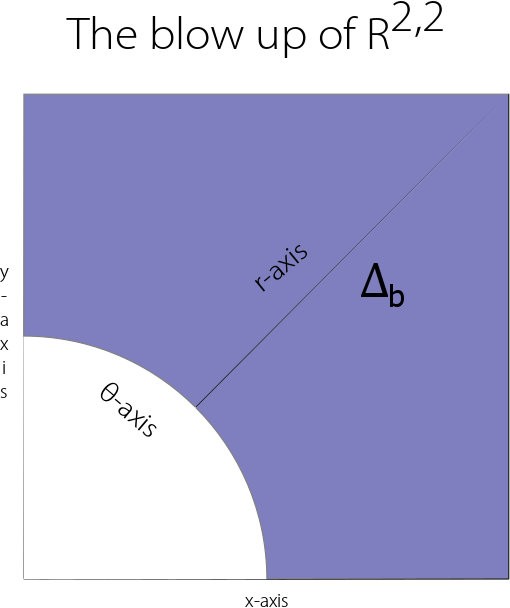
\includegraphics[width=100mm]{drawing5.png}
\end{center}
Today we are going to discuss the concept of blowing up and manifolds with corners. As a motivational example, let us consider the case of $\R^{2}$'s parametrization under the polar coordinates. The map is given by
\begin{align}
 \R^{*}\times  \mathbb{S}^{1}\rightarrow \R^{2}: (r,\theta)\rightarrow (r\cos(\theta),r\sin(\theta))
\end{align}
But the map cannot be globally bijective because the cylinder $R^{*}\times \mathbb{S}^{1}$ and the plane $\R^{2}$ are not homeomorphic. In particular we have
\begin{align}
(0,\theta)\rightarrow (0,0),\forall \theta\in \mathbb{S}^{1}
\end{align}
in which the whole circle is identified with a point. We have the following diagram:
\begin{center}
	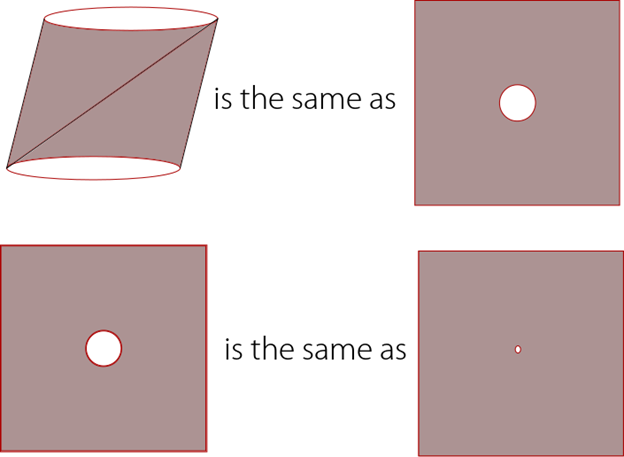
\includegraphics[width=100mm]{drawing6.png}
\end{center}
What we are really interested is to use the cylinder as a model of the punctured plane without the origin by identifying the other end of the cylinder with a circle around the origin. Technically,  by doing this we are replacing the singularity point at the origin with a circle to form a new space. We can write it formally as follows:
\begin{align}
[\R^2, 0]=\{\R^{2}-(0,0)\}+\{\R^{2}-(0,0)\}/\R^{+}
\end{align}
Here the left hand side is the ``blowed up" plane. The group $\R^{+}$ acts on the punctured plane by radial scaling. And the quotient space is a circle.

Now let us introduce some notation. We let
\begin{align}
\R^{n,k}=[0,\infty)^{k}\times \R^{n-k}, \mathbb{S}^{n-1, k}=\mathbb{S}^{n-1}\cap \R^{n,k}
\end{align}
\example
In particular,  $\R^{2,2}$ is the positive quadrant on $\R^{2}$. If we blow up the origin like we did for $\R^{2}$, the result is $[\R^{2,2},0]$. We can represent it using the following diagram using line (124):
\begin{center}
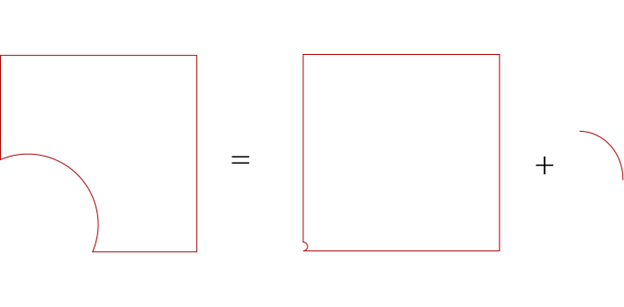
\includegraphics[width=120mm]{drawing8.png}
\end{center}
All we did is removing the origin, then replaced it by a quarter circle. Now analogous to the $[\R^{2},0]$ case we have a polar coordinate map:
\begin{align}
F:[\R^{2,2},0]\rightarrow [0,\infty)\times \mathbb{S}^{1,2}:
\end{align}
such that in the region $(\R^{2,2}/\{0\})/\R^{*}$ (the quarter circle), the map is given by
\begin{align}
[\omega]\rightarrow (0,\frac{\omega}{|\omega|}), \omega\in (\R^{2,2}/\{0\})/\R^{*}
\end{align}
and in the region outside of $0$ it is the ordinary polar coordinate map:
\begin{align}
[\omega]\rightarrow (|\omega|,\frac{\omega}{|\omega|}), \omega\in (\R^{2,2}-\{0\})
\end{align}
In other words, $F$ is just polar coordinates with $r=0$ included as before. It is clear that $F$ is bijective and $F,F^{-1}$ are both $C^{\infty}$. So $F$ is a differeomorphism.

\definition
Another name for $[\R^{2,2},0]$ given by Melrose is $[0,\infty)^{2}_{b}$. This is an example of \textit{Manifold with Corners}.

\example
We want to understand Example 6 in more detail. Let us consider the following neighborhoods of a point in $[\R^{2,2},0]$.
\begin{center}
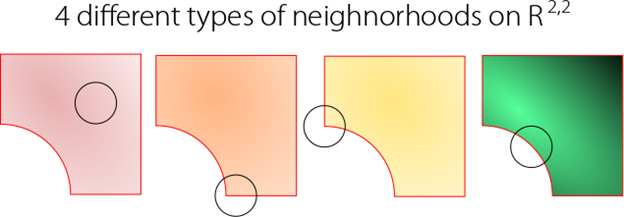
\includegraphics[width=120mm]{drawing 21.png}
\end{center}
In the red graph the neighborhood is locally the same as
\begin{align}
[r_1, r_2]\times [\theta_1, \theta_2]
\end{align}
In the orange graph the neighborhood is locally the same as
\begin{align}
[r_1, r_2]\times [0, \theta_1)
\end{align}
In the yellow graph the neighborhood is locally the same as
 \begin{align}
 [r_1, r_2]\times (\theta, \theta_2)
 \end{align}
 so in general it is a product of two half intervals. We may conclude that:
 \lemma
 For any point $p\in [0,\infty]^{2}_{b}$, its neighborhood will be a product of open intervals, closed intervals, or half-open, half closed intervals. In other words, $\forall p\in [0,\infty]^{2}_{b}$, there exists a subset $\mathcal{U}$ such that $\mathcal{U}\cong \R^{2,k}$ for some $k=0,1,2$.


 \definition Now we can define manifold with corners. This is just the usual manifold definition with $\R^{n}$ replaced with $\R^{n,k}$. Then we are done.

 \discussion Let us now move on to $\Psi DO$ defined on non-compact manifolds. For the simplest example, let us consider $M_{0}=[0,\infty)$. We can attach a cylinder end on the left hand side to form $\R$:
 \begin{center}
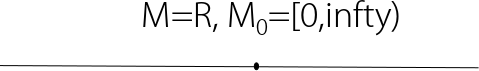
\includegraphics[width=120mm]{drawing22.png}
 \end{center}
 A typical Dirac operator is given by
 \begin{align}
D=\frac{1}{i}\partial_{t}, M_{0}=\R
 \end{align}
 We can perturb it a little to produce a second order elliptic operator. Let us consider
\begin{align}
E=D^{2}+\epsilon^{2}=-\partial_{x}^{2}+\epsilon^{2}, M_{0}=\R
 \end{align}
This is an elliptic pseudo-differential operator and we can write out its inverse:
 \begin{align}
P^{-1}\phi(t)=\int e^{i(t-t')\cdot \tau}(\tau^2+\epsilon^2)^{-1}\phi(t')dt'd(\frac{\tau}{2\pi}), \phi\in L^{2}(M_0)
 \end{align}
where $d(\frac{\tau}{2\pi})$ is the reduced density of $\tau$. In other words, formally we have
\begin{align}
P^{-1}=\int e^{it\cdot \tau} (\tau^2+\epsilon^2)^{-1}\widehat{\phi}(\tau), \phi\in L^{2}(M_0)
\end{align}
We now discuss the general philosophy of Richard Melrose. The idea is as follows: For a non-compact manifold with boundary, we can attach a cylinder to the boundary as we did in Lecture 1 and 2. But working with the cylinder is somehow inconvenient, because we need exponential decay condition on the cylinder part, plus we need to consider how the compact part and the cylinder part interact with each other. So we might want to find some way to get around with this. To see how bad the situation could be, let us consider the following diagram:
\begin{center}
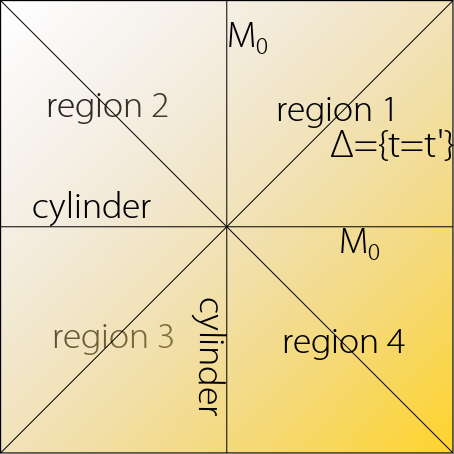
\includegraphics[width=100mm]{drawing23.png}
\end{center}
In order to define $P^{-1}$ properly on $M$ using conormal distribution, we have to work with 4 regions in $M\times M$, namely the compact times compact, non-compact times compact, non-compact times non-compact, compact times non-compact, etc. So we have 4 different behaviours to analyze for every pseudo-differential operator defined on $M$.  This is is not something we would like.

To summarize the analytical side, we have the following chart:
\begin{center}
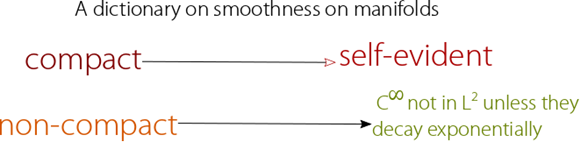
\includegraphics[width=140mm]{drawing24.png}
\end{center}
Therefore want we have incentive to convert non-compact case to the compact case. We cannot really convert a non-compact manifold to a compact manifold, as the two are topologically different. But we can compactify it after putting a cap after re-scaling using an exponential map:\\
This is the manifold before (the disks would extend to infinity):
\begin{center}
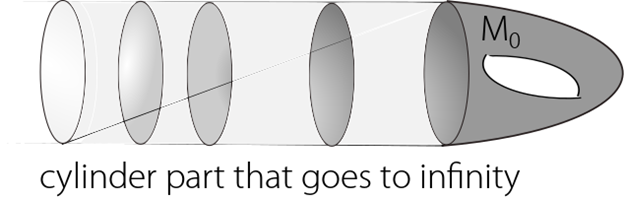
\includegraphics[width=100mm]{drawing14.png}
\end{center}
and this is the manifold after rescaling:
\begin{center}
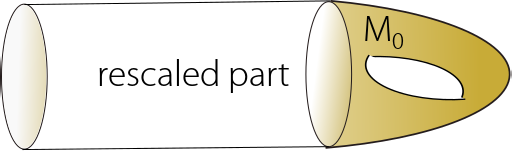
\includegraphics[width=100mm]{drawing26.png}
\end{center}
To do it we use a change of variable:
\begin{align}
x=e^{t}\in (0,1), t\in M=\R^{-}=(-\infty,0)
\end{align}
This transformed the infinite region
\begin{align}
(-\infty, t_{0})\rightarrow (0, x_{0})
\end{align}
\discussion Now we can define this rigorously:
\definition Let $M=M_{0}\cup Y\times (-\infty,0]$, Let $X=M_{0}\cup Y\times [0,1)$ under the rescaling map. After compatification we have $X'=M_{0}\cup Y\times [0,1]$.
\discussion
Topologically there is not much happening at here, $M\cong X$ is obvious; and $X,X'$ only differ by the cap. To recover $M$ to just need to let $M=X/{\partial X}$. But geometrically there is a huge difference. To see this let us consider $D$ again. We let
\begin{align}
D=\frac{1}{i}\sigma(\partial_{t}+A)=\frac{1}{i}\sigma(x\partial_{x}+A)
\end{align}
Here by chain rule we have
\begin{align}
\partial_{t}\phi&=\frac{\partial x}{\partial t}\partial_{x}\phi\\
&=e^{t}\partial_{x}\phi\\
&=x\partial_{x}\phi\\
&\rightarrow \partial_{t}=x\partial_{x}
\end{align}
analogously we have
\begin{align}
dx&=\frac{\partial x}{\partial t}dt\\
&=xdt\\
&\rightarrow \frac{dx}{x}=dt
\end{align}
Therefore geometrically things have changed. For example the metric is now give by
\begin{align}
g=dt^{2}+g_{y}\leftrightarrow (\frac{dx}{x})^{2}+g_{y}^{2}
\end{align}
\discussion
A natural question is whether the index of $D$ is not changed under such a transformation. This is asked by Adam. Prof. Loya answered in affirmative. In short, by using this transformation we have a new dictionary:
\begin{center}
Conditions on $D, \phi(t)\leftrightarrow$ Conditions on $D, \phi(x)$ being Fredholm, $L^{2}$, etc
\end{center}
Similarly, we have:
\begin{center}
$D:H^{\infty}(M, E)\rightarrow H^{\infty}(M, F)\leftrightarrow D: H^{\infty}_{b}(X, E)\rightarrow H^{\infty}_{b}(X,F)$
\end{center}
and earlier we have concluded that (APS theorem):
\theorem
The index of a Dirac operator with appropriate boundary conditions on $M$ is given by $$Ind D=\int^{b}_{M}AS-\frac{1}{2}\eta(0)$$
In this setting the same theorem would hold, but mind that with $x=e^{t}$ the regularization now takes $x^{z}$ instead. This is important: The index formulas for $(D,x)$ on $X$ correspond to index formula for $(D,t)$ on $M$.

\discussion
We now go back to philosophy. We can think after rescaling we essentially attached $M$ with a collar. So the essential question is how the collar compatification works versus (non-compact) cylinder. The cylinder gives us difficulty because if we want to let $D$ be Fredholm, we often need to impose extra boundary conditions. For example, the well known Dirichlet boundary condition dictates that $Du=v, u|_{\partial M}=0$, etc. For $\R^{2}$ this can be solved with separation of variables. But at $M$ in general it is not explicitly solvable because $D$ can be no longer elliptic on the boundary, and we would need so called $\textit{non-local conditions}$. For example in this case we could want
$$
B(u|_{\partial_{M}})=0, B\in \Psi^{0}
$$

\discussion
Let us go back to the case discussed earlier. Let
\begin{align}
P=D^2+\epsilon^2, P^{-1}=\int e^{i(t-t')\cdot \tau}(\tau^2+\epsilon^2)^{-1}d\tau dt'
\end{align}
and let $M=[0,\infty)^{2}=\R^{2,2}=[0,\infty)^{2}_{b}$ discussed earlier.  If we make the change of variable, then we would have
\begin{align}
P^{-1}&=\int e^{i(\log(x)-\log(x')}(\tau^2+\epsilon^2)d\tau \frac{dx'}{x'}\\
&=\int e^{i\log(\frac{x}{x'})\tau}(\tau^2+\epsilon^2)^{-1}d\tau\frac{dx'}{x'}\\
&=\int e^{iz\cdot \tau}(\tau^{2}+\epsilon^{2})^{-1}d\tau, z=\log(\cot(\theta))
\end{align}
where the last line comes from the fact we are using the kernel.
\discussion
We now observe the map
\begin{align}
F: (0,\frac{\pi}{2})\rightarrow (-\infty, \infty): \theta\rightarrow z=\log(\cot(\theta))_{z}
\end{align}
can be visualized as follows:
\begin{align}
(x,x')\rightarrow \theta\rightarrow \textrm{slope}\rightarrow \frac{1}{\textrm{slope}} \xrightarrow{\log} z
\end{align}
Correspondingly we have the following diagram:
\begin{center}
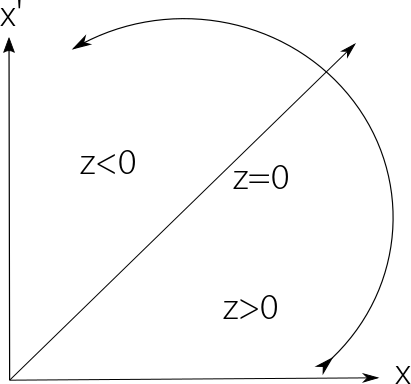
\includegraphics[width=100mm]{drawing15.png}
\end{center}
Now instead of working with $(r,\theta)$ on $[\R^{2,2},0]\cong [0,\infty)_{r}\times [0,\frac{\Pi}{2}]_{\theta}$, we can actually let $(r,z)$ to be the coordinates. And it is clear that now $z$ is the normal coordinate for $\Delta_b$ equal to $z=0$.  Thus we have the following diagram:
\begin{center}
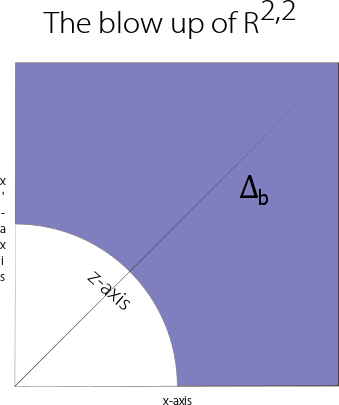
\includegraphics[width=100mm]{drawing17.png}
\end{center}
Now the transformation made $\mathcal{U}=[\R^{2,2},0]\cong [0,\infty)_{r}\times (-\infty,\infty)_{z}$.  We can now re-interpret $P^{-1}$ in terms of conormal distribution we learned last semester:
\begin{align}
P^{-1}|_{\mathcal{U}}=\int e^{iz\cdot \tau}(\tau^{2}+\epsilon^{2})^{-2}d\tau d\mu, \mu=\frac{dx'}{x'}
\end{align}
In other words we now regard $\mu$ as a density. We want to know what is the order of its principal symbol:
\lemma
\begin{align}
a(r,z,\tau)=(\tau^2+\epsilon^2)^{-2}\in S^{-2}
\end{align}
\proof
This is `clear' as we are working with inverse of a polynomial.
\qed
\discussion
We are naturally concerned what happens when $\theta=0$ and $\theta=\frac{\pi}{2}$. Now observe that we have
\begin{align}
P^{-1}|_{\mathcal{U}}=\frac{i}{2\pi i}\int e^{iz\cdot \tau}(\tau+i\epsilon)^{-1}(\tau-i\epsilon)^{-1}d\tau d\mu, \mu=\frac{dx'}{x'}
\end{align}
Notice that we have $iz(a+ib)=-zb+iza$. Therefore the integral has exponential decay and is well defined. Its only singularities are when $\tau=\pm i\epsilon$, see the diagram:
\begin{center}
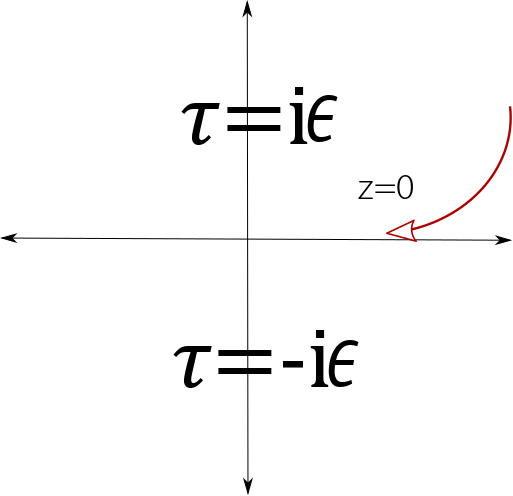
\includegraphics[width=100mm]{drawing16.png}
\end{center}
Therefore we can evaluate its kernel using a contour integral and let the four sides to go to infinity so that the boundary terms vanishes. In doing so we are fixing $z$ and integrating over $\tau$. This integral can also be evaluated via other means, like differentiation under integral sign. Here is the diagram for the contour integral:
\begin{center}
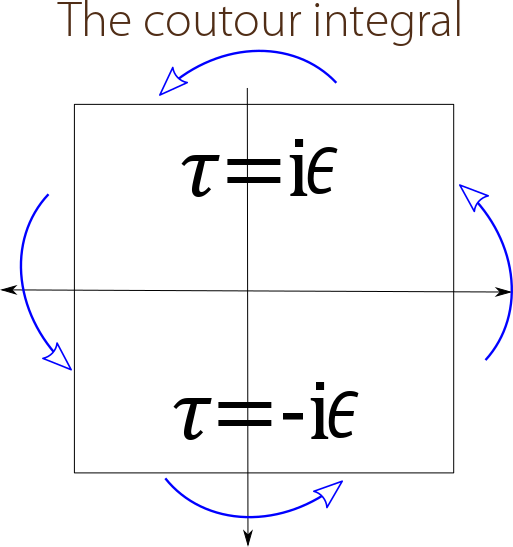
\includegraphics[width=100mm]{drawing18.png}
\end{center}
Now calculating the residue we get
\begin{align}
P^{-1}(\tau,z) = \begin{cases} e^{-z\epsilon}*\frac{1}{2\epsilon} &\mbox{if } z>0 \\
e^{z\epsilon}*\frac{1}{2\epsilon} & \mbox{if } z<0. \end{cases}
\end{align}
Recall that we have $z=\log(\cot[\theta])$ in the beginning. Therefore $e^{z}=\cot[\theta]$. Shifting $z$ into $\theta$ we have:
\begin{align}
P^{-1} = \begin{cases} \frac{\tan(\theta)^{\epsilon}}{2\epsilon} &\mbox{if } 0\le \theta<\frac{\pi}{4} \\
\frac{\cot(\theta)^{\epsilon}}{2\epsilon} & \mbox{if } \frac{\pi}{4}\le \theta\le \frac{\pi}{2} \end{cases}
\end{align}
Now by elementary calculus we have
\begin{align}
\tan[\theta]\sim \theta f(\theta), \cot[\theta]\sim (\frac{\pi}{2}-\theta)g(\theta), f,g\in C^{\infty}, f(0),g(0)=1
\end{align}
and we can regard $\theta, \phi=\frac{\pi}{2}-\theta$ as local coordinates near the boundary of $\mathcal{U}=[\R^{2,2},0]$.  So we can re-write $P^{-1}$ as
\begin{align}
P^{-1} = \begin{cases} \theta^{\epsilon} \tilde{f}(\theta) &\mbox{if } 0\le \theta<\frac{\pi}{4} \\
\phi^{\epsilon}\tilde{g}(\phi) & \mbox{if } 0\le \phi<\frac{\pi}{4} \end{cases}, \tilde{f}(\theta)=f(\theta)^{\epsilon}, \tilde{g}(\phi)=g(\phi)^{\epsilon}
\end{align}
We comment that $P^{-1}$ is not a smooth function on the whole space. Indeed we have the following diagram:
\begin{center}
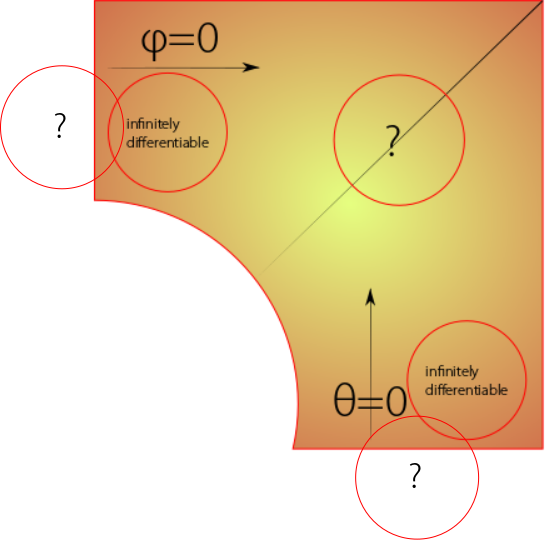
\includegraphics[width=100mm]{drawing25.png}
\end{center}
From the diagram we can see that $P^{-1}$ is infinitely differentiable near the two sides, as we have the expression $\phi^{\epsilon}*C^{\infty}(\phi)$ or $\theta^{\epsilon}*C^{\infty}(\phi)$ available. But this expression is not available in the region vertical to the diagonal and on the two sides. This is also clear from the perspective of conormal distribution.

\definition
We now write $P^{-1}\in \Psi^{-2,\epsilon}_{b}$, where $-2$ denotes the order of the $b-\Psi DO$, and $\epsilon$ denotes the $\textit{order of vanishing}$.

\example
\begin{align}
E&=\frac{1}{2\pi}\int_{\tau \in \R}e^{-(x-x')\tau} (i\tau+A)^{-1}i\sigma d\tau\\
&=\frac{1}{2\pi}p(x)p(x')\int e^{(x-x')\tau}(i\tau+A)^{-1}i\sigma d\tau
\end{align}
This is a familiar example. In other words the kernel of $E$ is $(i\tau+A)^{-1}$. Therefore $E\in \Psi^{-1}(X)$. Similarly we have $e^{-tD^+D^-}\in \Psi^{-\infty, \infty}(X)$.

\definition We now define $\Psi^{m, \epsilon}(X)$ rigorously by
\begin{align}
\Psi^{m,\epsilon}(X)=I^{m}(M^{2}_{b}, \Delta_{b})
\end{align}
and the $\epsilon$ index means we can write the kernel as
\begin{align}
h(\theta)+r^{\epsilon}h(r,\theta)
\end{align}
on $[0,1]_{r}\times [0,\frac{\pi}{2}]_{\theta}$. A good execrise is to show the exponential decay quality of $P^{-1}$ from the $\epsilon$ term.

\section{Lecture 4:Geometry of manifold with corners}
Recall from last time that we discussed
\begin{align}
P^{-1}=\frac{1}{2\pi}\int e^{(t-t')\cdot \tau}(\tau^{2}+\epsilon^{2})^{-1}d\tau, t\in (-\infty, 0)
\end{align}
Now using the transformation $x=e^{t}, x'=e^{t'}$ we change it into
\begin{align}
P^{-1}=\frac{1}{2\pi}\int e^{i\log(\frac{x'}{x})}(\tau^2+\epsilon^2)^{-1}d\tau, x,x'\in (0,1)
\end{align}
We recall that the space we are working with is
\begin{align}
X^2=[0,\infty)^2
\end{align}
The main issue as we noticed last time is $P^{-1}$ is smooth when $x\rightarrow 0$ or $x'\rightarrow 0$, as we can tell the term $\log(\frac{x'}{x})$ goes to infinity either way and the integral vanishes via Riemann-Lesbegue lemma. But it is not smooth when $x,x'$ both goes to $0$ in the same time.
\remark
If $x=x'$ then $t=t'$, and the integral still exists as the exponential term is $1$. What is exactly bad about it?
\discussion This corresponds to the bad behaviour of $P^{-1}$ near the point $(0,0)$ as we can see from the diagram:
 \begin{center}
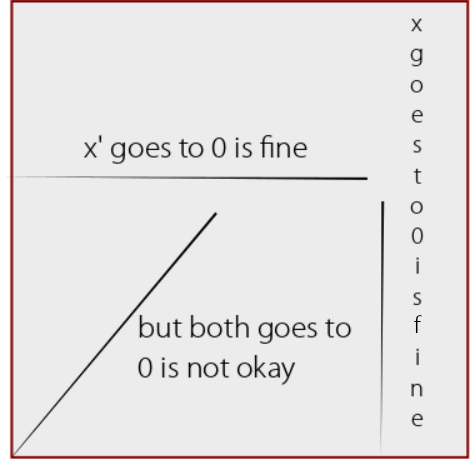
\includegraphics[width=100mm]{drawing28.png}
 \end{center}
There is a treatise on this topic by Elmar Schrohe called SG-pseudo-differential operators.  To resolve this problem Melrose introduced polar coordinates to blow up the origin. Now we have the following picture from last time   :
\begin{center}
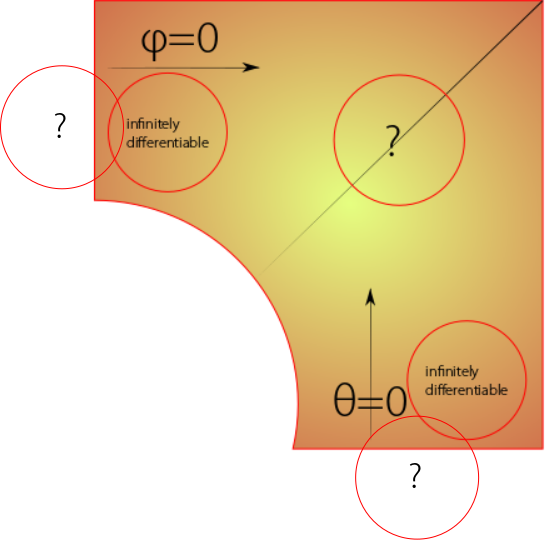
\includegraphics[width=100mm]{drawing25.png}
\end{center}
The goal for today is to discuss blow-up and manifold with corners in general as well as the so called $b$-vector fields.
\definition
A $n$-dimensional $\textbf{general manifold with corners}$ is a paracompact, Hausdauff, topological space such that for each $p\in X$, there exists an open set $\mathcal{U}\subseteq X$ and a homeomorphism $F:\mathcal{U}\rightarrow \R^{n,k}$ such that $F(p)=0$.  We further require these coordinate patches to be compatible. The space locally is a product of half intervals.
\definition Here $n-k$ is called the $\textbf{codimension}$ of the manifold at $p$.
\example
We recall the earlier example from last class:
\begin{center}
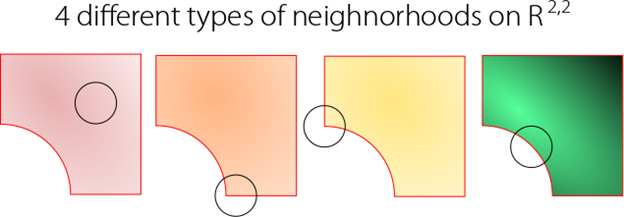
\includegraphics[width=120mm]{drawing29.png}
\end{center}
For the red one the neighborhood is locally $\R^{2}$, while for the orange one the neighborhood is locally $[0,\infty)\times [0,\infty)$. The codimension for the red one is $0$, for the orange one is $2$, and so on. Similarly the dented circle can be viewed as $\mathbb{S}^{1}\cap [0,\infty)^{2}$.
\example
Here is a very famous example, a so called ``tear drop''.
\begin{center}
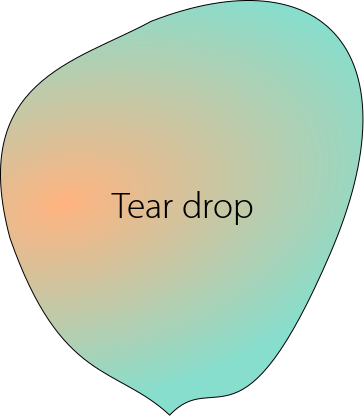
\includegraphics[width=100mm]{drawing30.png}
\end{center}
The tear drop is an example of a $\textbf{tied manifold}$ as the boundary tied around a point. If we analyse the geometry of the tear drop, in the inside near any point the neighborhood is given by $\R^{2}$, and on the boundary it is given by $[0,\infty)\times \R$ .  On the corner it is of the form $[0,\infty)^{2}$.

Why this is a canonical example? The $\textit{bad part}$ of the tear-drop is that its boundary hypersurface is no longer a submanifold with corners, and nor is it a finite union of submanifold with corners. We want to avoid this kind of phenomenon from happening in future. We need a definition of a submanifold:

\definition
A submanifold $Y\subseteq X$ is a subset such that $\forall p\in Y$, there exists a coordinate patch $F:\mathcal{U}\rightarrow \R^{n_1,K_1}\times \R^{n_2,k_2}$ and it satisfies
\begin{align}
F:\mathcal{U}\cap Y\rightarrow \R^{n_1,k_1}\times \{0\}
\end{align}
\example
Let us consider the familiar example:
\begin{center}
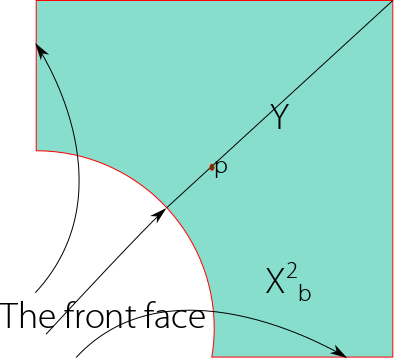
\includegraphics[width=100mm]{drawing32.png}
\end{center}
Here $X^{2}_b=[0,\infty)_{r}\times [0,\frac{\pi}{2}]_{\theta}$, and $Y=[0,\infty)\times \frac{\pi}{4}$. If we choose local coordinates $z=\theta-\frac{\pi}{4}$, then clearly we have
\begin{align}
F:\mathcal{U}\rightarrow [0,\infty)\times (-\frac{\pi}{4},\frac{\pi}{4})=R^{1,1}\times \R^{1}, F|_{Y}=[0,\infty)\times \{0\}_{z}
\end{align}
Therefore $Y$ is a submanifold of $X^{2}_{b}$. Similarly we may analyze the $\textit{front face}$.  The front face is the union of three boundary submanifolds. The quarter circle boundary equal to $\{0\}\times [0,\frac{\pi}{2}]$, and the vertical/horizontal boundary  equal to  $\{0\}\times [0,\infty)$ or $[0,\infty)\times \{0\}$ respectively. This is $\textit{nice}$ as we can properly analyze it piece by piece!
\example
Let us return to the tear drop example: If we regard a neighborhood near the singular point of the tear drop as $\R^{2,2}$, then we have
\begin{align}
F|_{Y\cap \mathcal{O}}\rightarrow \{x_1=0\}\bigcup \{x_2=0\}
\end{align}
In particular it is not of the form $\R^{n,k}$. This is not what we wanted because $Y$ is one piece only, and it is not of form $\R^{n,k}$. If $Y$ is given by the union of two pieces then this is actually okay. This is a bit hard to believe, and let us see it via the diagram:
\begin{center}
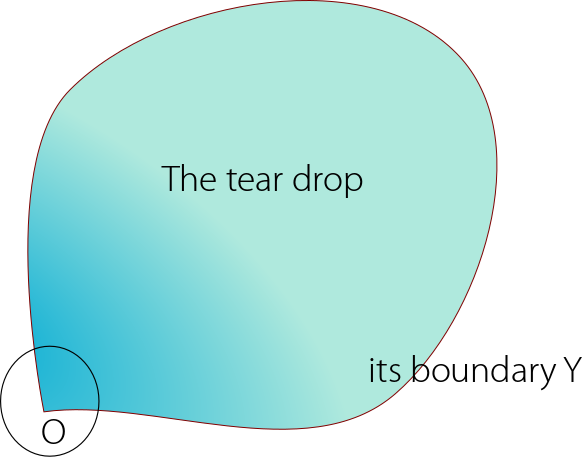
\includegraphics[width=100mm]{drawing33.png}
\end{center}
and the two piece tear drop:
\begin{center}
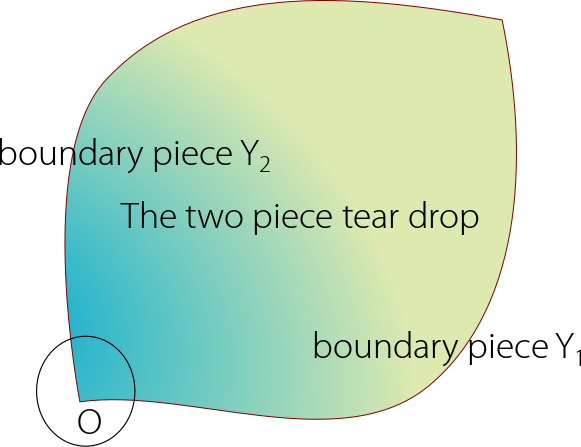
\includegraphics[width=100mm]{drawing34.png}
\end{center}
\example
To make it even simpler, let us consider another example provided by Prof. Loya:
\begin{center}
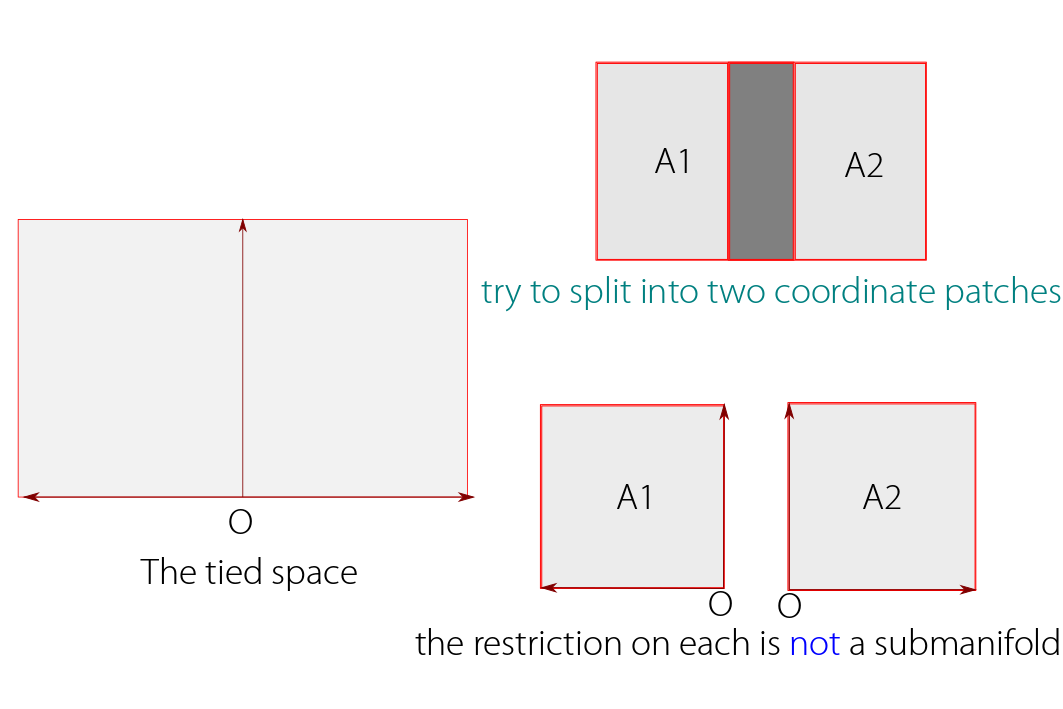
\includegraphics[width=150mm]{drawing69.png}
\end{center}


\discussion
The above discussion motivates the following definitions:

\definition
A boundary hypersurface $H$ of a general manifold with corners is a codimensional $1$ subset such that $H\subset \partial X$.

\definition
A manifold with corners is a general manifold with corners such that $\partial X$ is the union of finitely many boundary pieces.

\example
Let us see some elementary examples: The first is $\R^{2,2}$, the second is $\mathbb{D}^{3}$, the third is $X^{2}_{b}$:

\begin{center}
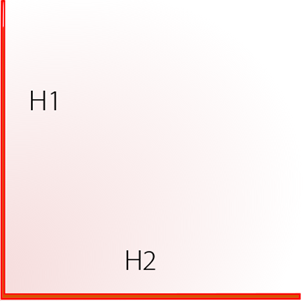
\includegraphics[width=50mm]{drawing35.png} 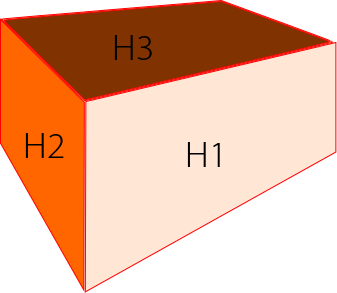
\includegraphics[width=50mm]{drawing36.png}
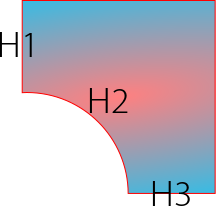
\includegraphics[width=50mm]{drawing37.png}
\end{center}
\discussion
Hence forth we only work with manifolds with corners. We want to define the cotangent bundle on $X$. Here is the motivation: Let $f:\R\rightarrow \R$. Now if $p\in \R$, we have
\begin{align}
f(x)\approx f(p)+\frac{df}{dx}(p)dx
\end{align}
In other words, we can approximate $f(x)-f(p)$ via:
\begin{align}
f(x)\approx f(p)+df+O(|x-p|^2)
\end{align}
We can use this to establish an equivalence relationship. Let $p\in \R$, then
\begin{align}
f\sim g\leftrightarrow f-g \textit{  vanishes at second order}\approx O(x-p)^2
\end{align}
Now let $C_{p}=\{f\in C^{\infty}(\R)|f(p)=0\}$. Then we may define $T_{p}^{*}(\R)$ by
\definition
\begin{align}
T_{p}^{*}(\R)=C_{p}/\sim
\end{align}
Formally for all $f\in C^{\infty}(\R)$, we have $[f-f(p)]_{p}=df_{p}$. We observe that
\begin{align}
df_{p}&=[\frac{df}{dx}(p)(x-p)]_{p}\\
&=\frac{df}{dx}(p)[x-p]_{p}\\
&=\frac{df}{dx}(p)dx_{p}
\end{align}
Therefore formally we have
\begin{align}
df=\frac{df}{dx}*{dx}
\end{align}

\definition
If $X$ is a manifold with corners and $p\in X$, we have
\begin{align}
C_p=\{f\in C^{\infty}(X)|f(p)=0\}
\end{align}
and we introduce the same equivalence relationship:
\begin{align}
f\sim g\leftrightarrow f-g \textit{  vanishes at second order}\approx O(x-p)^2
\end{align}
Then we define $T^{*}X, TX$ by
\begin{align}
T^{*}X=\bigcup_{p\in M}T^{*}_{p}X, T(X)=(T^{*}X)^{*}
\end{align}

\example
If $\mathcal{U}$ is a coordinate neighborhood of $X$, then we have $\mathcal{U}\cong \R^{n,k}$. Now for all $p\in \mathcal{U}$, we have
\begin{align}
\alpha \in T^{*}_{p}X\leftrightarrow \alpha=\sum a_{i}dx_{i}+\sum b_{i}dy_{i}, a_i, b_i\in \R
\end{align}
as well as
\begin{align}
v\in T_{p}X\leftrightarrow v=\sum a_{i}\partial_{x_i}+\sum b_{i}\partial_{y_i}, a_i, b_i\in \R
\end{align}
\discussion
We now switch back to the cylinderal view point:
\begin{center}
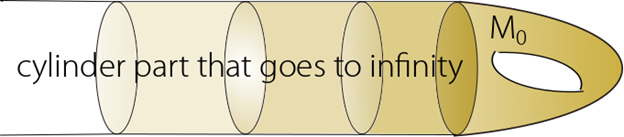
\includegraphics[width=100mm]{drawing38.png}
\end{center}
as well as the rescaling we did:
\begin{center}
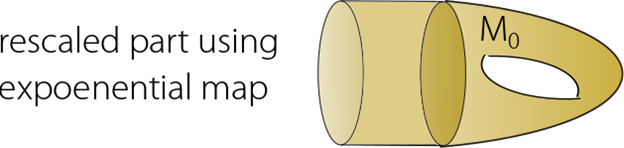
\includegraphics[width=100mm]{drawing39.png}
\end{center}
Earlier the cylinderal part is of the form $Y\times (-\infty, 0]_{t}$. Use rescaling with $x=e^{t}$, we have the vector field isomorphism:
\begin{align}
\partial_{t}\rightarrow x\partial_{x}, \partial_{y_i}\rightarrow \partial_{y_i}
 \end{align}
 The question is how to make sense of terms like $x\partial_{x}$ as a vector field. We think them geometically. Notice that we have
 \begin{align}
\textrm{span} \{x\partial_{x}, \partial_{y_i}\}=\{ v\in C^{\infty}(X, TX): v|_{\partial X}\in TY\}
 \end{align}
 This motivates us to define an important space, the space of all such vector fields:

 \definition
 If $X$ is a manifold with corners, then we define
\begin{align}
V_{b}(X)=\{v\in C^{\infty}(X, TX)|\forall \textrm{ boundary hypersurface } H, v|_{H}\in C^{\infty}(H, TH)\}
\end{align}
Let us see this via an example:

\example
If $\mathcal{U}\cong \R^{n,k}$ is the image of a patch, then $V_{b}(X)$ is locally spanned by
\begin{align}
x_1\partial_{x_{1}}\cdots x_k\partial_{x_{k}}, \partial_{y_1}\cdots \partial_{y_{n-k}}
\end{align}
because we have
\begin{align}
v\in V_{b}(\mathcal{U})\rightarrow v=\sum^{k}_{i=1}a_{i}\partial_{x_i}+\sum^{n-k}_{j=1}b_{j}\partial_{y_j}, a_{i}|_{x_{i}=0}=0
\end{align}
Therefore using intermediate value theorem we get $a_{i}=x_{i}a'_{i}$ at the origin and (186) holds. But we still have difficulty on how to define principal symbol rigorous. This will be addressed in Lecture 5.

\section{Lecture 5:The ${}^b$-category invented by Melrose}
This time we will talk about ${}^{b}TX$ and  ${}^{b}T^{*}X$, blow ups, b-differential operators. We will discuss $b$-$\Psi DO$s next week.

Let us go back to our canonical example. Let
\begin{align}
D=\frac{1}{i}\sigma(x\partial_{x}+D_{y}), D_{y}=i\partial_{y}
\end{align}
\begin{center}
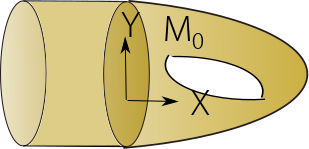
\includegraphics[width=70mm]{drawing40.png}
\end{center}
Now a typical tangent vector field near the boundary is of the form
\begin{align}
v=\{x\partial_{x}, \partial_{y} \}\in C^{\infty}(X, TX), v|_{x=0}=v|_{\partial_x}\in C^{\infty}(\partial X, T\partial X)
\end{align}
This motivates us to define $V_{b}(X)$ in Definition 14. Let us see more examples. Let $X=\R^{2,2}$, then it has boundary $x_{i}=0$:
\begin{center}
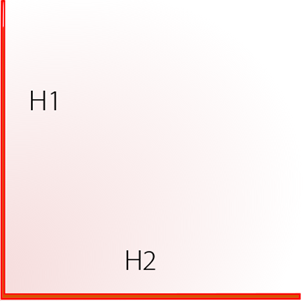
\includegraphics[width=50mm]{drawing35.png}
\end{center}
Now we have
\begin{align}
V_b(X)=\{v=a_1(x)\partial_{x_1}+a_2(x)\partial_{x_2}|\forall H_i, v|_{H_i}\in C^{\infty}(H_i, TH_i)\}
\end{align}
Now similar to (187) we have
\begin{align}
v|_{x_1=0}=a_{1}(0,x_2)\partial_{x_1}+a_{2}(0,x_2)\partial_{x_2}
\end{align}
We know that $a_{1}(0,x_2)=0$, Therefore since $a_1(x_1,x_2)\in C^{\infty}(X)$,  via intermediate value theorem we have near $x_1=0$, $a_{1}(x_1, x_2)=x_{1}\tilde{a_1}(x)$. Similar reasoning conclude that $a_2(x)=x_2\tilde{a_2}(x)$.  Now we conclude that
\begin{align}
\therefore v\in V_{b}(X)\leftrightarrow v=x_1\tilde{a_1}(x)\partial_{x_1}+x_2\tilde{a_2}(x)\partial_{x_2}, a_1, a_2\in C^{\infty}(X)
\end{align}
In general $V_b(X)$ is introduced because we want to study manifolds with corners.

\discussion For us to analyze $\R^{2,2}$ we can envision us attaching to cylinders such that $\R^{2,2}\rightarrow (0,1]^{2}$. This can be done via a double change of variables:
\begin{align}
x_1=e^{t_1}, x_2=e^{t_2}, \partial_{t_i}\rightarrow x_{i}\partial_{x_i}, \partial_{y_i}\rightarrow \partial_{y_i}
\end{align}
In general if we want to study a manifold with multi-cylinderal ends, it is equivalent to study of its compatification into a manifold with corners with compatification of $b$-differential operators.

\example
Let us consider $X=\R^{2}$ considered as attaching two cylinders to $\R^{2,2}=(-\infty, 0]^2$. Then after compatification we get $I^{2}$:
\begin{center}
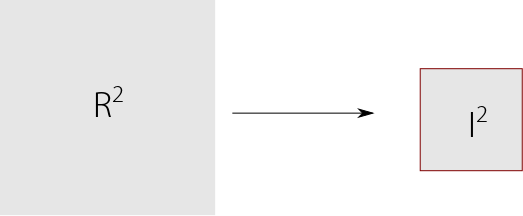
\includegraphics[width=100mm]{drawing41.png}
\end{center}
In particular we have an associated map of vector fields:
\begin{align}
\partial_{t_1}\rightarrow (x_1+1)(x_1-1)\partial_{x_1}, \partial_{t_2}\rightarrow (x_2+1)(x_2-1)\partial_{x_2}
\end{align}
which we get analogous to what we did earlier. These vector fields span $V_{b}(I^2)$ after the transformation. A natural question is why there is a product $(x_1+1)(x_1-1)$ in equation 194. But this is clear from the fact that $I^2$ has $x_1=\pm 1$ as its boundary. The same phenomeon clearly extends to $\R^{3}$:

\example Here is the analogous picture for $\R^3\rightarrow I^3$:
 \begin{center}
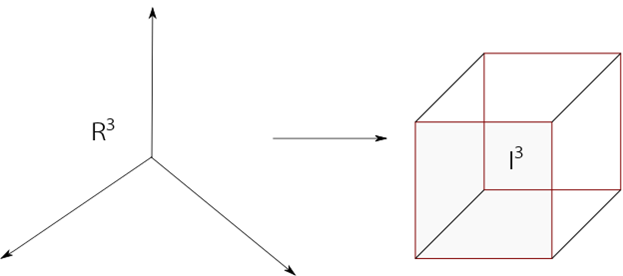
\includegraphics[width=100mm]{drawing42.png}
 \end{center}
Notice that it is vital that we need the axis to be 90 degree apart from each other. This is because we want to have the metric given by
\begin{align}
dt_1^2+dt_2^2+dt_3^2\rightarrow (\frac{dx_1}{x_1})^2+(\frac{dx_2}{x_2})^2+(\frac{dx_3}{x_3})^2
\end{align}
And in general we can use it to generalize APS paper:
\begin{align}
\sum^{k}_{j=1}dt_{j}^{2}+g_{y}\rightarrow \sum_{j=1}^{k}\frac{1}{i}\sigma_{j}\partial_{t_j}+A_{y}
\end{align}
\discussion
We shall now discuss the $\textit{b-differential operators}$, which is always modelled by a cylinder. Recall that a differential operator $P$ of order $m$ on $M$ can be expressed by
\begin{align}
P=\sum_{|\alpha|+|\beta|\le m}a_{\alpha \beta}\partial^{\alpha}_{t}\partial_{y}^{\beta}
\end{align}
and its symbol is given by
\begin{align}
\sigma(P): T^{*}(M)\rightarrow \R
\end{align}
such that its $m$-order principal symbol is given by
\begin{align}
\sigma_{m}(P)(\xi_1 dt+ \sum \xi_j dy_j)=\sum_{|\alpha|+|\beta|=m}a_{\alpha \beta}(t_1, y)(i\xi_1)^{\alpha}(i\xi_2)^{\beta}, y=(\xi_2\cdots \xi_n)
\end{align}
This is the standard definition of the principal symbol. We want to study this on $X$, which is a compatified version of $M$. We want to define
\begin{align}
P\in \textrm{Diff}^{m}_{b}(X), P:C^{\infty}(X)\rightarrow C^{\infty}(X)
\end{align}
Now use a change of coordinates, we have:
\begin{align}
P=\sum_{|\alpha|+|\beta|\le m}a_{\alpha \beta}(x\partial_{x})^{\alpha}\partial_{y}^{\beta}
\end{align}
and we can try to analyze it using equation (199): We have
\begin{align}
\sigma_{m}(P)(\xi_1\frac{dx}{x}+\sum \xi_{j}dy_j)=\sum a_{\alpha \beta}(x,y)(i\xi_1)^{\alpha}(i\xi_2)^{\beta}
\end{align}
The main question is whether this is still well-defined. Of course we have to prove this. However we face a conceptual difficulty. We know that
\begin{align}
\textrm{span} \{dt, dy_1 \cdots dy_n\}=T^{*}_{p}(M)
\end{align}
But is it true that we have
\begin{align}
\textrm{span} \{\frac{dx}{x}, dy_1 \cdots dy_n\}=T^{*}_{p}(X)?
\end{align}
It turns out that we need to work with a new space. To define this space, let us recall how to form a vector bundle using given sections:

\example
Let $f(x)=\frac{1}{x}$, we want a line bundle over $\R$ such that $f(x)=\frac{1}{x}$ is a global section of the line bundle $V$. The trouble is $f(x)$ is not really well-defined at $x=0$ and we have a singularity point there:
 \begin{center}
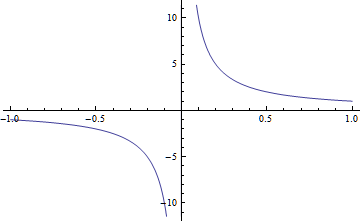
\includegraphics[width=100mm]{drawing43.png}
 \end{center}
 We want to use a trick to treat $f(x)$ as a whole and avoid the singularity point. For all $p\in \R$, let us formally define
 \begin{align}
F=\{ a(x)f(x)|a\in C^{\infty}(\R) \}, \tilde{F}_{p}=\{a(x)f(x)|a(p)=0\}
 \end{align}
and then we can define $V_{p}$ point-wise by
 \begin{align}
V_{p}=F/\tilde{F}_{p}
 \end{align}
 This is another genius invention by Melrose, as no one else has realized this, including prominent people like Wolfgang Scholtz. In fact, we have an isomorphism given by the evaluation map:
 \begin{align}
V_{p}\cong \R: a(x)f(x)\rightarrow a(p)[f]
 \end{align}
because the difference of two elements in the same class is 0:
 \begin{align}
a(p)=b(p)\rightarrow (a-b)(x)f(x)\in \tilde{F}_{p}\rightarrow a\sim b
 \end{align}
 Therefore the map is injective, and it is clearly surjective. So it is an isomorphism. Thus $[f]$ gives the global section of the vector bundle $V=\{\bigcup V_{p}\}$.  In short, we get around the singularity issue by considering $F$, where $1=x*\frac{1}{x}\in F, x=a(x)$ is still defined algebraically at $x=0$.

 It is clear that the choice of $\frac{1}{x}$ is not important at here, any other function like $x^{10}$ or $x^{3/5}$ can work with no difference. But after all we want $\frac{dx}{x}, dy_1\cdots dy_n$ be a local trivialization of a vector bundle. So how to construct it?

 \example
 We approach this problem by dualization, as direct construct is somewhat difficult. In other words we want to construct the space of vector fields spanned by $(x\partial_{x},\partial_{y_n})$, then flip back to its dual space. We want to construct a vector bundle such that elements in $V_{b}(X)$ are the sections of the vector bundle:
 \begin{center}
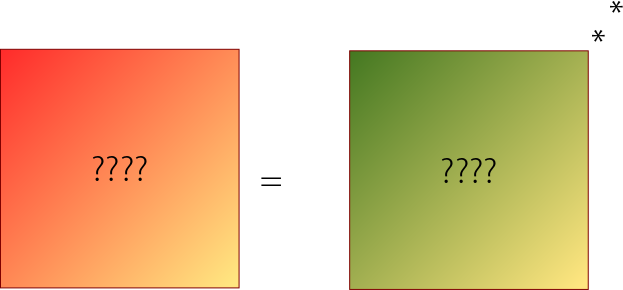
\includegraphics[width=100mm]{drawing44.png}
\end{center}

 \definition
 Let $p\in X$, let $\mathcal{V}_{p}(X)$ defined by:
 \begin{align}
 \mathcal{V}_{p}(X)=\{\sum_{\textrm{finite}} a_{i}v_{i}|a_{i}\in C^{\infty}(X), v_{i}\in V_{b}(X) , a_{i}(p)=0\}
 \end{align}
 then we define $\BTX$ by:
  \begin{align}
\BTX_{p}=V_{b}(X)/\mathcal{V}_{p}(X), \BTX=\bigcup_{p\in X} \BTX_{p}
  \end{align}

\example
 It is important to notice that a different space
  \begin{align}
U_{b}(X)_{p}=\{ av|a\in C^{\infty}(X), a(p)=0, v\in V_{b}(X)\}
\end{align}
 does not work because this is not even a vector space.
 \discussion
 Now by definition we have $[x\partial_{x}]_{p}, [\partial y_{j}]_{p}$ forms a basis of $\BTX_{p}$. Thus a section near $\partial X$ is of the form
 \begin{align}
v=\sum ax\partial_{x}+\sum b_{j}\partial_{y_j}, a, b_{j}\in C^{\infty}
 \end{align}
We proceed to define the $b$-cotangent bundle ${}^{b}TX^{*}$:

\definition
${}^{b}TX^{*}$ is the dual space of $\BTX$.  Now if $p\in \partial X$, then $\{\frac{dx}{x}, dy_{i}\}$ span ${}^{b}TX^{*}$ near $p$.

\discussion We may finally define the principal symbol rigorously:

\definition
For all $P\in \textrm{Diff}^{m}_{b}(X)$, we have
 \begin{align}
\sigma_{m}(P): {}^{b}TX^{*}\rightarrow \R
 \end{align}
 defined by
 \begin{align}
\forall P, \xi, P=\sum a_{\alpha \beta}(x\partial x)^{\alpha} \partial_{y}^{\beta}, \xi=\xi_1\frac{dx}{x}+\sum \xi_{j}dy_j
 \end{align}
 we have
 \begin{align}
 {}^{b}\sigma_{m}(P)(\xi)=\sum_{|\alpha|+|\beta|=m}(i\xi(x\partial_{x}))^{\alpha}(i\xi(\partial_{y}))^{\beta}=\sum_{|\alpha|+|\beta|=m}(i\xi_1)^{\alpha}(i\xi_{2\cdots n})^{\beta}
 \end{align}

 \discussion
 We now want to define $b$-operators in general as well as $b$-densities. This is in general not so easy as we want them to be coordinate invariant. Again let us see this through an example:

\example
Let $V$ be a finite dimensional $\R$-vector space. We recall that we defined $\Omega^{2}(V)$ by
 \begin{align}
 \Omega^{2}(V)=\{a|\omega|^{2}, a\in \R , \omega\in \wedge^{n}(V)\}
 \end{align}
 The ones that are important to us is when $a=1$, and we define $\Omega^{1}V=\Omega(V)$.  This showed up when we integrate:
 \begin{align}
\int f(x)dx_1\cdots dx_n, dx_1\cdots dx_n=|dx_1\wedge \cdots \wedge dx_n|\in \Omega^1(T^{*}_{p}\R^{n})
 \end{align}
 We have the following theorem:
 \theorem
 The following statement holds:
 +
 \begin{align}
\Omega^{\alpha}(V)\otimes \Omega^{\beta}(V)=\Omega^{\alpha+\beta}(V)
 \end{align}
 +
\begin{align}
(\Omega^{-\alpha}V)^{*}=\Omega^{\alpha}(V)
 \end{align}

+
\begin{align}
\Omega^{0}(V)\cong \R
\end{align}

+
\begin{align}
\Omega^{\alpha}(V\oplus W)=\Omega^{\alpha}(V)\otimes \Omega^{\alpha}(W)
\end{align}

+
\begin{align}
(\Omega^{\alpha}V)^{*}=\Omega^{-\alpha}(V)=\Omega^{\alpha}(V^{*})
\end{align}

\proof
For the proof of (218,220,221) it suffice to use a basis of $V$ and expand out all the terms. For a proof of (219, 222), notice that we have the evaluation map
\begin{align}
f: \langle a, b\rangle\rightarrow a*b
\end{align}
this finishes the proof.
\qed
\definition
For now though, let $X$ be a manifold with corners, let $V$ be a vector bundle over $X$. Then we have
\begin{align}
\Omega^{\alpha}(V)=\bigcup_{p\in X}\Omega^{\alpha}(V_{p})
\end{align}
In particular, let $V={}^{b}T^{*}X$, then we have
\begin{align}
{}^{b}\Omega^{\alpha}(X)=\Omega^{\alpha}({}^{b}TX)=\bigcup_{p\in X}\Omega^{\alpha}({}^{b}T_{p}X)
\end{align}
is a so called $\textit{b-density bundle}$.

\discussion Now let ${}^{b}\Omega_{X}$ be the $b$-densities, and $\mu\in C^{\infty}(X, {}^{b}\Omega_{X})$. Locally if $Y$ is the boundary hypersurface, then we have:
\begin{center}
	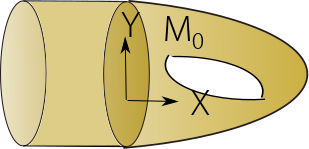
\includegraphics[width=70mm]{drawing40.png}
\end{center}
\begin{align}
\mu=\alpha|\frac{dx}{x}\wedge dy_1 \wedge \cdots dy_{n-1}|\in \wedge^{n}({}^{b}T^{*}X), \alpha\in C^{\infty}(X)
\end{align}
and we certainly want to integrate things like this. Now suppose $\mu$ is positive, then we have
\begin{align}
L^{1}(X)=\{f:X\rightarrow \C|\int |f|_{X}<\infty\}
\end{align}
but after re-scaling this is the same as
\begin{align}
L^{1}(M)=\{f:M\rightarrow \C|\int |f|_{M}<\infty\}
\end{align}
where $M$ is the original space plus the cylinder:
\begin{center}
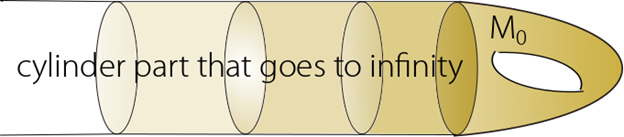
\includegraphics[width=100mm]{drawing38.png}
\end{center}
We want to comment that this space is $\textbf{independent of}$ the choice of coordinates because $\alpha\in C^{\infty}(X)$ is bounded over $X$, and $X$ is compact. Originally, we have
\begin{align}
L^{p}(M)=\{f:M\rightarrow \C|\int |f|^{p}dtdy<\infty\}
\end{align}
Now moving from $M$ to $X$ via $x=e^{t}$ we have $dt=\frac{dx}{x}, dy=dy$, then
\begin{align}
L^{p}(M)=\{f:X\rightarrow \C|\int |f|^{p}\frac{dx}{x}dy<\infty\}
\end{align}
The best way to view this is to think of it as the density of the $b$-cotangent bundle. In general, the philosophy is to give a name to every object using a geometric object. For closed manifold it is just a density, and for APS case a density of the b-cotangent bundle. Clearly this also carries for manifolds with corners.

Let us now fix $\mu\in \wedge^{n}({}^{b}T^{*}X)$ that is positive. We want to define $b$-differential operator:

\theorem
We have
\begin{align}
P\in \textrm{Diff}^{m}_{b}(X)\leftrightarrow P=a+\sum_{|I|\le m} v_{i_1}\circ \cdots \circ v_{i_k}, a\in C^{\infty}(X), v_{j}\in V_{b}(X)
\end{align}
such that
\begin{align}
P:C^{\infty}(X)\rightarrow C^{\infty}(X)
\end{align}

\exercise
As an execrise, you should prove this using Equation (201). The hint is to show it using finitely many vector fields and have a coefficient in front.

\theorem
If $P\in \textrm{Diff}^{m}_{b}(X)$, then $P^{*}\in \textrm{Diff}^{m}_{b}(X)$.
\definition
We want to define the following to be the space of all functions with super-exponential decay:
\begin{align}
\dot{C^\infty}(X)=\{f(x)\equiv 0,\forall x\in \partial X\}, \partial^{\alpha}f(x)\equiv 0, \forall x\in \partial X
\end{align}
So in particular a constant function $f\equiv 1$ would not be smooth on $X$ as it does not vanish near the boundary.

\discussion
We want to comment that the $L^{1}$ decay condition we have corresponds to exponential decay condition on cylinder. To see this we can ignore the factor from $Y$ by treating it as a constant, and focus on $x$. We know that $f(x,y)=f(x)$ is integrable on $X$:
\begin{align}
\int_{Y}\int_{0}^{1}\frac{1}{x}|f(x)|dx<\infty\rightarrow \int^{1}_{0}\frac{1}{x}|f(x)|dx<\infty
\end{align}
Therefore we can write $f(x)=xg(x)$ where $g(x)\in L^{1}(0,1]$.  Similarly if $f\in L^{p}(X)$, then we would have $f=xg^{p}(x)$, $g\in L^{1}$.

In general, since $f$ is bounded on $X$, for all $N$ we can simply let $f(x,y)=x^{N}g_{N}(x,y)$ on $(0,1]$.  But we know that $x=e^t$, so we have $f(t,y)=e^{Nt}g_{N}(t)$. This way we get $\textit{super-exponential decay}$ because $g_{N}(t)$ has to decay with a magnitude of $e^{Nt}$.  This is faster than exponential decay as this works for any $N$.

\example
As an example, we let
\begin{align}
f(x,y)=e^{-t^2}g(t,y), g_{N}(x,y)=g(t,y)\in C^{\infty}([0,1])\times Y
\end{align}
Now if we let $\dot{C^\infty}(X)$ to denote the space of all functions with super exponential decay, we can define the inner product
\begin{align}
\langle f, g\rangle=\int_{X} f\overline{g}d\mu
\end{align}
and this will be well defined because of super exponential decay, though this is much stronger than needed.

\discussion
Now to go back to the theorem, we have $\langle Pf, g\rangle=\langle f, P^{*}g\rangle, \forall f,g\in C^{\infty}(X)$ by definition. We shall prove the theorem by steps: The motivation is the dual of $\partial_{t}$ is $-\partial_{t}+\alpha$, where $\alpha \in C^{\infty}(X)$ is a divergence. So we would need
\begin{align}
\int \partial_{t}f\overline{g}d\mu=\int f (-\partial_t+\alpha )\overline{g} d\mu
\end{align}
This divergence term is coming from $d\mu$. If we write it out, we would have
\begin{align}
\int \partial_{t}f\overline{g} A| dx\wedge \cdots dy_{n-1}|&=\int \partial_{t}fA\overline{g}|dx\wedge \cdots \wedge dy_{n-1}|\\
&=\int f (-\partial_{t})(\overline{g}A)|dx\cdots dy_{n-1}|+\int_{\partial X}fA\overline{g}|dx\wedge \cdots \wedge dy_{n-1}|\\
&=\int f(-\partial_{t}\overline{g})A|dx\wedge \cdots \wedge dy_{n-1}|+\int f\overline{g} (-\partial_{t}A)|dx\wedge \cdots \wedge dy_{n-1}|\\
&=\int f(-\partial_{t}\overline{g})d\mu+\int f\overline{g}(-\partial_{t}\log(A))d\mu\\
&=\int f(-\partial_{t}+\alpha)\overline{g}d\mu, \alpha=-\partial_{t}\log(A)
\end{align}
Here from (238) to (239), the second term vanishes since $g\equiv 0$ on $\partial X$.
\proof
+
We let
\begin{align}
P=\sum_{|I|\le k}V_{i_0}\cdots V_{i_k}, V\in V_{b}(X)
\end{align}
We have the following Lemma. If $V\in V_{b}(X)$, then there exist $a\in C^{\infty}(X)$ such that
\begin{align}
V^{*}=a-V
\end{align}
For a proof, I think this is basically what we did earlier in this page. However this is more complicated as we have to deal with
 \begin{align}
\int x\partial_{x}f\overline{g}A|dx\wedge \cdots dy_{n-1|}
 \end{align}
and after integration by parts we would get more residual terms from $\partial_{x}(x\overline{g}A)$.
+
As the second step, we use the fact that if $A_{i}$ are linear operators, we would have
 \begin{align}
(A_{1}\circ A_{m})^{*}=A_{m}^{*}\circ \cdots \circ A_{1}^{*}
 \end{align}
 as well as
 \begin{align}
  (A_{1}\cdots +\cdots A_{m})^{*}=A_{1}^{*}+ \cdots  +A_{m}^{*}
 \end{align}
 And we can simply the case to the situation that $m=1$.

 +
 As the last step, we use a partition of unity to construct $V$ globally over $X$ via the coordinate charts. We can write $V$ as
  \begin{align}
V=\sum \phi_{j}v_{j}, (\phi_{j}v_{j})^{*}= a_{j}-\phi_{j}v_{j}
  \end{align}
Then we have
 \begin{align}
P=\sum_{|i|\le m}v_{i1}\circ \cdots \circ v_{ik}\rightarrow P^{*}&=\sum_{i\le m}(-\overline{v}_{i1}+a_{i1})\circ \cdots \circ (-\overline{v}_{ik}+a_{ik})\\
&=\sum_{|i|\le m}W_{i1}\circ \cdots W_{ik}, W_{ij}\in V_{b}(X)
 \end{align}
 which finished the proof.
 \qed

 \discussion
 Here is another interesting fact. Notice that we can think of principal symbols as maps from the cotangent vector space to the reals. Let $v\in V_{b}X$, then for all $p\in X$, we have $v_{p}\in \BTX_{p}=({}^{b}T^{*}_{p}X)^{*}$. This enable us to view the $b$-tangent vector as a map:
 \begin{align}
v_{p}: {}^{b}T^{*}_{p}X\rightarrow \R
 \end{align}
 The prior discussion takes in a complexified version, in the sense that the map is to $\C$ instead of $\R$. Now the principal symbol for $v$ should be given by
  \begin{align}
\sigma_{p}(v)=iv_{p}
  \end{align}
and we can interpret it via (251).

\lemma
The object we defined here is exactly the principal symbol map:
\begin{align}
\sigma_{p}(v)={}^{b}\sigma_{1}(v)_{p}
\end{align}

\proof
Here is the idea. Near $\partial X$, we have
\begin{align}
V=ax\partial_{x}+\sum b_{j}\partial_{y_j}
\end{align}
Therefore for $p\in X$, we have
\begin{align}
\sigma_{p}(V)=a(p)(x\partial_x)+\sum b_{j}(p)\partial_{y_j}: {}^{b}T^{*}_{p}X\rightarrow \C
\end{align}
Let us see, for example if $\xi=\xi_1\frac{dx}{x}+\sum \xi_j dy_j$, then we have
\begin{align}
\sigma_p(v)(\xi)&=a(p)i(x\partial_x)(\xi)+\sum b_{j}(p)\partial_{y_j}(\xi)\\
&=a(p)i\xi_1+\sum b_{j}(p)i\xi_{j}\\
&={}^{b}\sigma(v)(\xi)
\end{align}
\qed

We still need to show the invariance under coordinate change:
\theorem
Let $P\in \textrm{Diff}^{m}_{b}(X)$, if we write
\begin{align}
P=\sum_{|I|\le m} v_{i1}\circ \cdots \circ v_{ik}
\end{align}
Then for all $p\in X$, we have
\begin{align}
P=\sum_{|I|\le m} v_{i1}\circ \cdots \circ v_{ik}
\end{align}
as well as
\begin{align}
{}^{b}\sigma_{m}(P)=\sum_{|I|=m}{}^{b}\sigma_{1}(v_{i1})\cdots {}^{b}\sigma_{1}(v_{ik})
\end{align}
The coordinate invariance is now left as an exercise:

\exercise
Finish proving coordinate invariance, composition, adjoint, etc.

\discussion
This is essentially linear algebra and is done in Lecture 6 by Prof. Loya.

\discussion Next time we want to discuss $\textrm{Diff}^{m}_{b}$ in more detail, as well as real blow-ups. We would like to discuss conormal distributions on $X^{2}_{b}$. For example, why $A\in \Psi^{m}: C^{\infty}(X)\rightarrow C^{\infty}(X)$ can be interpreted via $(\pi_L)^{*}(K_{A}\pi_{R}^{*}\phi)$ would ends up to be $I^{m}(X^{2}_{b},\Delta, \Omega)\rightarrow C^{\infty}(X^{b}_{2}, \Omega)$ by extension via continuity? We also wish to remark that $(\pi_L)^{*}$ is not a fibration in general.


\section{Lecture 6: The $b$-principal symbol}
We now set out to prove coordinate invariance.
\definition
If $P\in \textrm{Diff}^{m}_{b}(X)$, with $P=\sum_{|\alpha|+|\beta|\le m} a_{\alpha \beta}(x\partial_x)^{\alpha} \partial_{y}^{\beta}$ in local coordinates. Then we have
\begin{align}
{}^{b}\sigma_{m}(P)(\xi)=\sum_{|\alpha|+|\beta|}a_{\alpha \beta}(i\xi_1)^{\alpha}(i\xi_2)^{\beta}, \xi=\xi_1\frac{dx}{x}+\sum^{n-1}_{j=1}\eta_{j}dy_{j}
\end{align}
\discussion
Adam suggested a different approach using the $\textit{exponential trick}$ or using linear algebra by working with framing. However Prof. Loya insist to carry on with his approach and see how it goes.

\theorem
The $b$-principal symbol of $P$ is coordinate invariant.

\proof
With the notation in Definition 19, we choose a coordinate patch in which $p$ is near $\partial X$. Notice that off the boundary $P$'s principal symbol is perfectly defined already. Now let $X=[0,1)_{X}\times Y$, and $P=\sum_{|\alpha|+|\beta|\le m} a_{\alpha \beta}(x\partial_x)^{\alpha} \partial_{y}^{\beta}$. On the coordinate patch, let $\xi_p\in T^{*}_{p}X, \xi=\xi_1\frac{dx}{x}+\sum^{n-1}_{j=1}\eta_{j}dy_{j}$. Let $f(x,y)=x_1(\log(x)-\log(x(p))+\sum y_{j}(\eta_{j}-\eta_{j}(p))$. Then we have
\begin{align}
f(p)=0, df_{p}=\xi(p)
\end{align}
Now we consider
\begin{align}
{}^{b}\sigma_{m}(P)(\xi(p))={}^{b}\sigma_{m}(P)(df(p))
\end{align}
We have the following little observation: If we let
\begin{align}
g=\frac{1}{m!}f^{m}
\end{align}
Observe that we have
\begin{align}
Pg=\frac{1}{m!}\sum_{|\alpha|+|\beta|\le m}a_{\alpha \beta}(x\partial_{x})^{\alpha}\partial_{y}^{\beta}(f^{m})|_{p}, Pg|_{p\in X}=i^{m}\frac{m!}{m!}\sum_{|\alpha|+|\beta|\le m}a_{\alpha \beta}(\xi_1)^{\alpha}\eta^{\beta}
\end{align}
We know that by (263) we have
\begin{align}
(x\partial_{x})^{\alpha}(\partial_{y})^{\beta}(f^{m})|_{p}=0, |\alpha|+|\beta|<m
\end{align}
Therefore we have
\begin{align}
(Pg)|_{p}={}^{b}\sigma_{m}(P)(\xi_p)
\end{align}
Now if $P$ takes form in other coordinates, the operation of $P$ on $g$ is the same. Therefore $P$ is coordinate invariant.
\qed
\discussion
We now prove composition, adjoint, etc. We notice that we can write
\begin{align}
P=\sum^{m}_{|I|\le m}v_{i1}\circ v_{i2}\cdots v_{ik}, (Pg)_{p}=\sum_{|I|=m}v_{i1}(p)(\xi_p)\cdots v_{ik}(p)(\xi_p)
\end{align}
We know that
\begin{align}
(v_0\circ \cdots \circ v_{k})f^{m}|_{p}=
\begin{cases} 0 &\mbox{if } k\le m \\
m!v_{i1}(p)(df)\cdots v_{ik}(p)(df) & \mbox{if }k=m \end{cases} \pmod{2}
\end{align}
and as a result we have
\begin{align}
{}^{b}\sigma_{m}(P)|_{{}^{b}T^{*}_{p}X}=\sum_{|I|=m}v_{i1}(p)\cdots v_{ik}(p)
\end{align}
as well as
\begin{align}
{}^{b}\sigma(P\circ Q)={}^{b}\sigma(P)\circ {}^{b}\sigma(Q)
\end{align}
Here is a graph of what we had been discussed:
\begin{center}
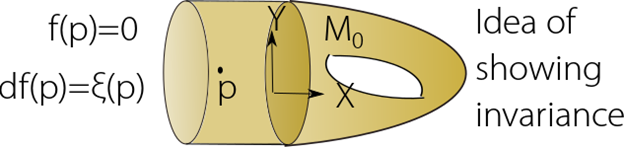
\includegraphics[width=100mm]{drawing45.png}
\end{center}
\discussion
We wish to discuss projective coordinates. They are special, useful coordinates on $X^{2}_{b}$. In fact, Prof. Melrose use this in his research all the time.

Recall that we blowed up $[0,\infty)^{2}$ to form $X^2_b$ by replacing the origin by a quarter circle:
\begin{center}
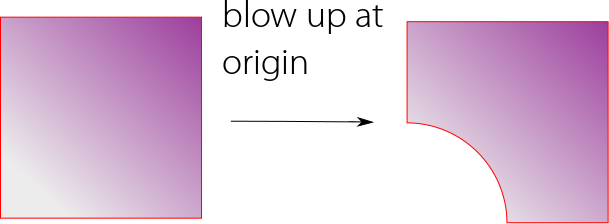
\includegraphics[width=100mm]{drawing46.png}
\end{center}
The ideal of projective coordinates is to identify the interval $[0,\frac{\pi}{2}$ of the angle with $[0,\infty)$ by a differeomorphism. Technically we project the angle to the point on the line through the angle to the origin:
\begin{center}
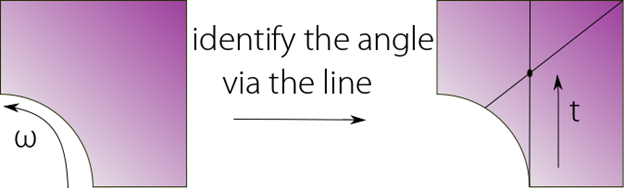
\includegraphics[width=100mm]{drawing47.png}
\end{center}
The idea now is to work with $\mathbb{S}^{1,2}=[0,\infty)^{2}\{0\}/\R^+$. Let $(\omega_1,\omega_2)$ denotes the original coordinate in the quarter circle, then $(1,t)=(1,\frac{\omega_2}{\omega_1})$ denotes the new coordinate when $\omega_1>0$. This kind of identification has advantage when we properly generalize to higher dimensions. Similar to what we did above, we can also try to use $\omega_2>0$, and the graph is as follows:
\begin{center}
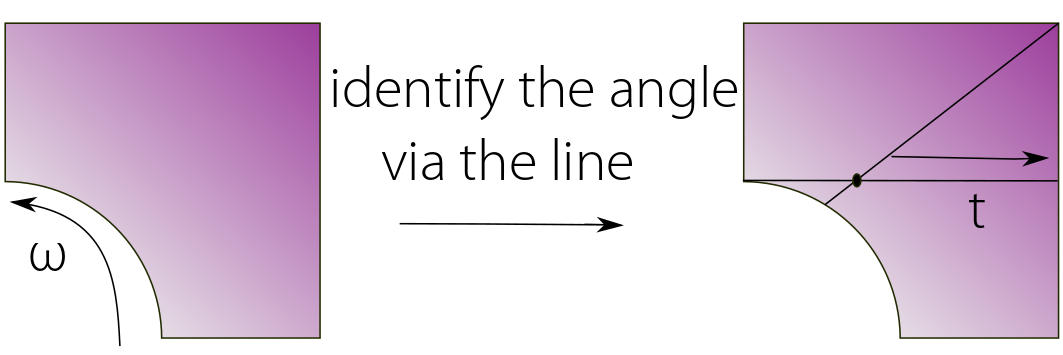
\includegraphics[width=100mm]{drawing48.png}
\end{center}
In general, we can also try other schemes like working with $\omega_1<0, \omega_2<0$, etc on the other parts of the plane. The graphs are mostly similar and here is a typical one:
\begin{center}
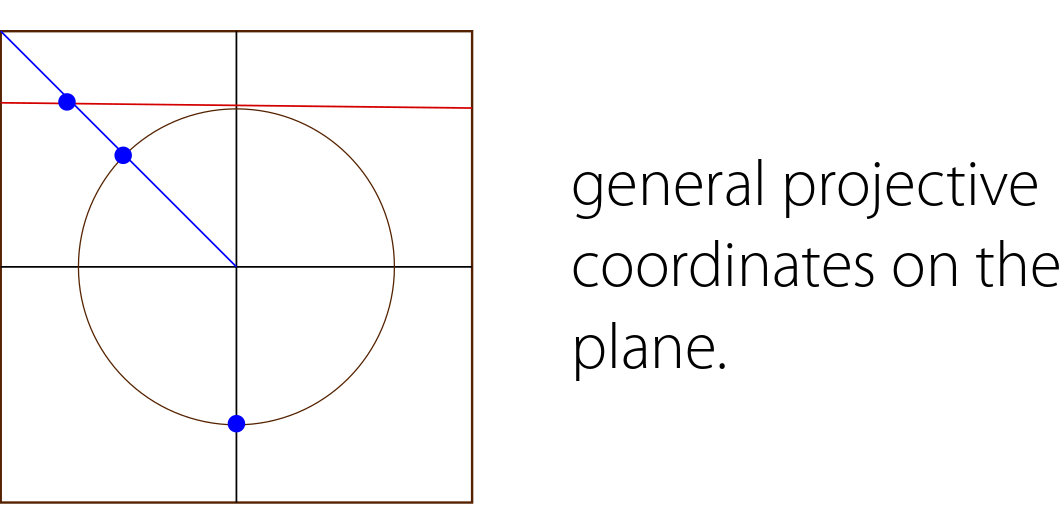
\includegraphics[width=100mm]{drawing49.png}
\end{center}
where we worked with the case $\omega_1<0, t=\frac{w_2}{w_1}$. What we really want to find out, however is the transformation map:
\begin{align}
(r,\omega_1,\omega_2)\rightarrow (r\omega_1,\frac{w_2}{w_1})
\end{align}
We should note that because we are working with the blowed up plane $X^{2}_b$, we should not confuse ourselves by using $x_1, x_2$ and treat them as real Euclidean coordinates. Now the transformation map is given by
\begin{align}
r\omega_1=z_1,\frac{\omega_2}{\omega_1}=z_2: \rightarrow r^{2}=z_1^2+z_1^2*z_2^2, r=z_1\sqrt{1+z_2^{2}}, \omega=(\frac{1}{\sqrt{1+z_2^2}},\frac{z_2}{\sqrt{1+z_2^2}})
\end{align}
However, this `plug in method' is quite ugly and very difficult to visualize. We want to come up with a geometric way to think about it.

Let us think this way. In the original $xy$-plane, we have $x$-axis given by $y=0$ and $y$-axis given by $x=0$. However in the blowed-up plane we have a different situation. For example, we can visualize the $z_2$ axis in the region $\omega_1>0$:
\begin{center}
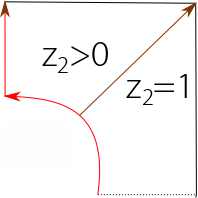
\includegraphics[width=50mm]{drawing51.png}
\end{center}
You might ask what is the use of this. We can see it more clearly by converting it to the $(z_1,z_2)$ picture:
\begin{center}
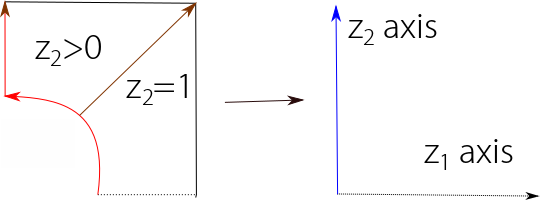
\includegraphics[width=100mm]{drawing52.png}
\end{center}
This is not really a trick. It is useful because we can express $z_1, z_2$ with respect to original coordinates in a nice way:
\begin{align}
z_1=r\omega_1, z_2=\frac{\omega_2}{\omega_1}
\end{align}
and we can think about this from the perspective of vector fields. If we let $x_1=r\omega_1, x_2=r\omega_2$, then we mapped vector fields via chain rule:
\begin{align}
x_1\partial_{x_1}\rightarrow z_1\partial_{z_1}-z_2\partial_{z_2}, x_2\partial_{x_2}\rightarrow z_2\partial_{z_2}
\end{align}
because using $x_1=z_1, x_2=z_1z_2$, by chain rule we have
\begin{align}
\partial_{z_1}&=\frac{\partial_{x_1}}{\partial_{z_1}}\partial_{x_1}+\frac{\partial_{x_2}}{\partial_{z_1}}\partial_{x_2}\\
&=\partial_{x_1}+z_{2}\partial_{x_2}\\
&\rightarrow  z_1\partial_{z_1}=x_1\partial_{x_1}+x_{2}\partial_{x_2}
\end{align}
which proved the first formula. The second follows analogously:
\begin{align}
\partial_{z_2}&=\frac{\partial_{x_2}}{\partial_{z_2}}\partial_{x_2}\\
&=z_{1}\partial_{x_2}\\
&\rightarrow z_{2}\partial_{z_2}=x_2\partial_{x_2   }
\end{align}

 \discussion
The point is that $b$-differential operators lift to blow up space. The change of coordinates are much easier. We would expect formulas like
\begin{align}
a_1(x_1,x_2)x_1\partial_{x_1}+a_2(x_1,x_2)\partial_{x_2}\rightarrow a_1(z_1z_2,z_2)z_1 \partial_{z_2}+a_{2}(z_1z_2,z_2)(\cdots)
\end{align}
In short, the transformation we have for $b$-vector fields are very nice.

\example
In the $b$-calculus, the projection map is no longer a fibration. This is totally different from the Euclidean case, as can be seen from the following diagram:
\begin{center}
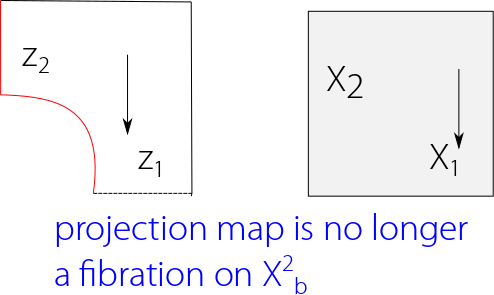
\includegraphics[width=100mm]{drawing53.png}
\end{center}
This cause an issue for us, because if we consider the left projection map:
\begin{align}
t=\pi_{L}(z_1, z_2)=z_1\cdot z_2
\end{align}
We would have the following diagram:
\begin{center}
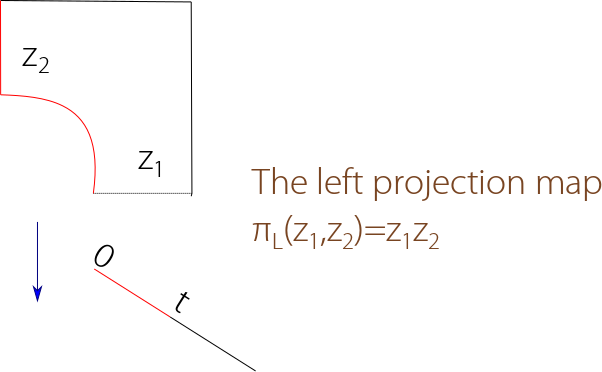
\includegraphics[width=100mm]{drawing54.png}
\end{center}
Consider the fiber over $t=0$, we would find it is the high-lighted red part in the diagram. We have
\begin{align}
z_1z_2=r\omega_1*\frac{\omega_2}{\omega_1}=r\omega_2
\end{align}
Therefore the fibre over $t=0$ would include $r=0$ and $\omega_2=0$. But we are working with the region $\omega_1>0$. So the only choice is to let $r=0$. In general, $b$-fibrations are no longer honest fibration away from the boundary. Similar to what we did at here, we can also consider the projective coordinates given by $\omega_2>0$. In this case we may use
\begin{align}
z_1=\frac{\omega_1}{\omega_2}, z_2=r\omega_2
\end{align}
instead. As a result the diagram the diagram we have would be different as well:
\begin{center}
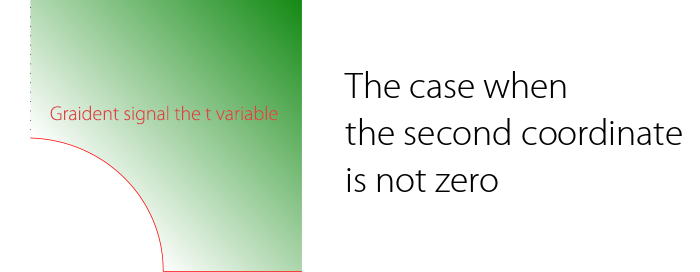
\includegraphics[width=120mm]{drawing56.png}
\end{center}

\example
We can analogously discuss the higher dimensional case, where we work with $\R^{n,k}$ and the angle space is $(\R^{n,k}/{0})/\R^{+}=\mathbb{S}^{n-1, k}_{\omega}$.  The whole space is now parametrized by
\begin{align}
[0,\infty)_{r}\times \mathbb{S}^{n-1,k}_{\omega}
\end{align}
and we can work with projective coordinates via various hyperplanes as we did before.  For example, now the coordinate patch $\mathcal{U}_{i}$ is defined by $\R^{n,k}_{z}\cap \omega_{i}\ge 0$. If we define $z_{i}=r\omega_{i}, z_{j}=\frac{\omega_{j}}{\omega_{i}},\forall j\not=i$, then we can discuss higher dimensional cases similar to what we did earlier. \\
 To recover, away from the front face we would have
\begin{align}
z_{i}=x_{i}, z_{j}=\frac{x_{j}}{x_{i}}, x_{i}>0
\end{align}
Just as what we had earlier.

\example
Here is a three dimensional case with $(\omega_1,\omega_2,\omega_3)$ be the radial coordinates and we project to $\omega_2>0$ by $(\frac{w_1}{w_2},1,\frac{w_3}{w_2})$,which we think of as $(\R^{3}/\{0\})/\R^{+}$:.

\begin{center}
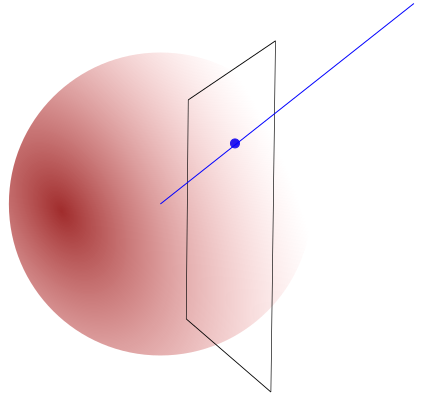
\includegraphics[width=100mm]{drawing50.png}
\end{center}

\example
Let $n=3, k=0$ and we have the following example. Here we use the half space $\omega_1>0$. The coordinate axis are shown in the following graph:
\begin{center}
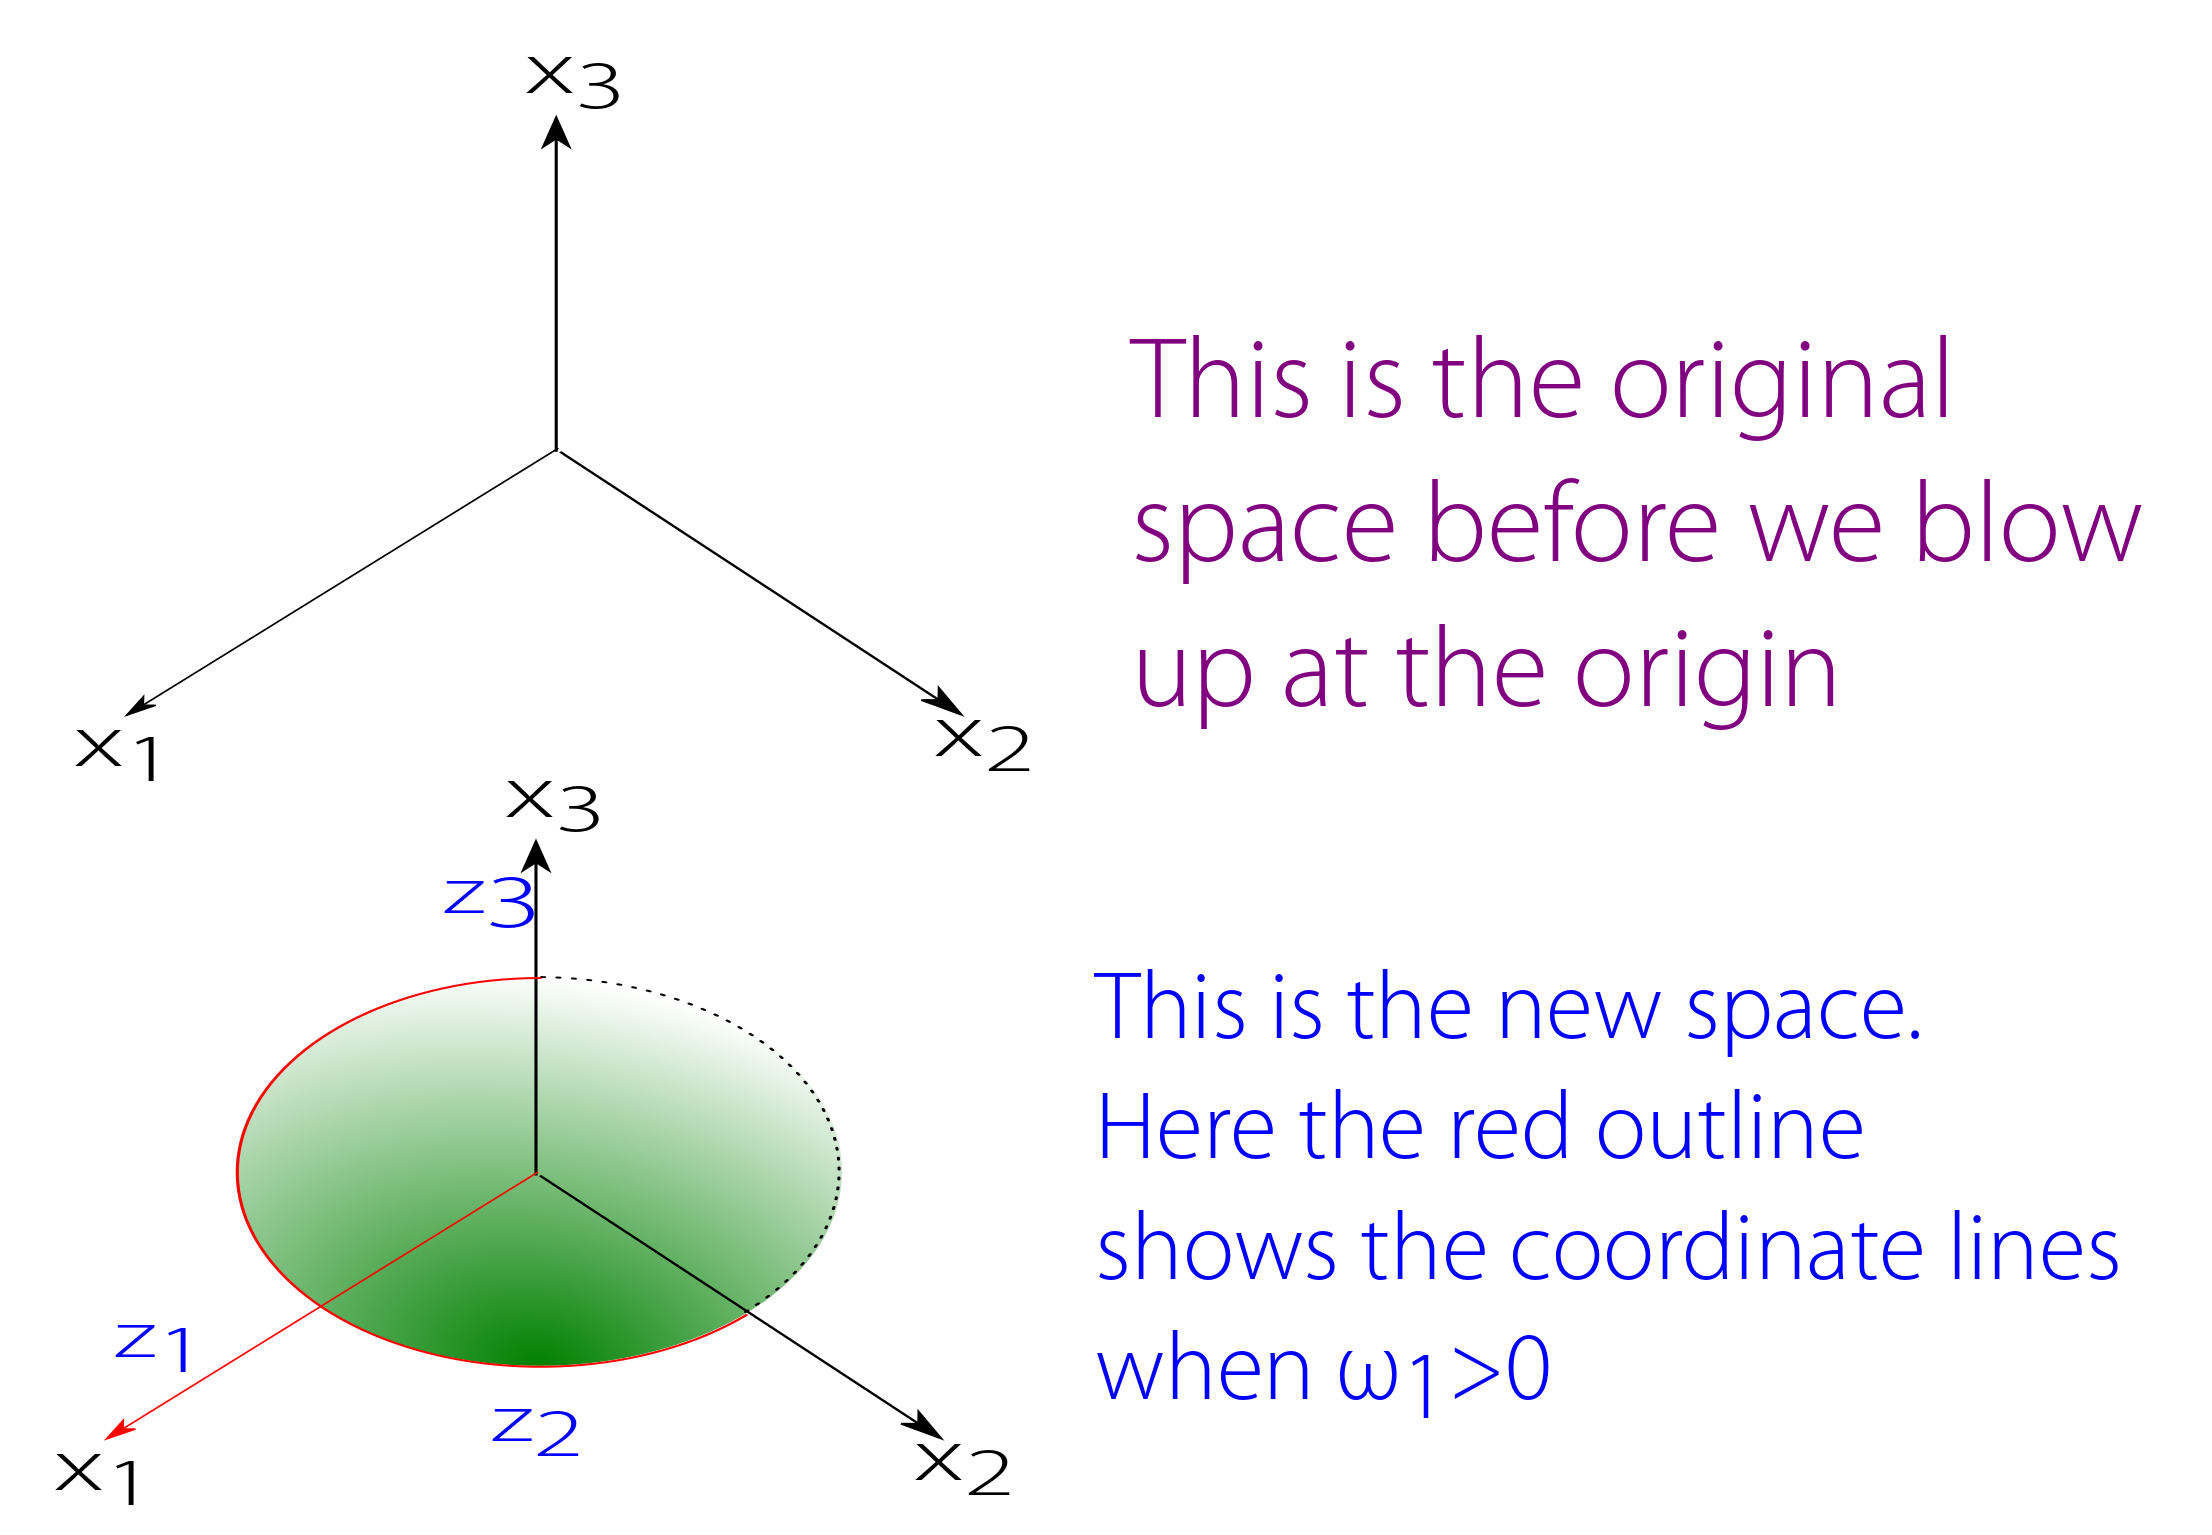
\includegraphics[width=120mm]{drawing58.png}
\end{center}
In this case we are  considering the ordinary left  projection map:
\begin{align}
\pi_{1,2}(x_1,x_2,x_3)\rightarrow (x_1, x_2)
\end{align}
which again fail to be a fibration after we switch to $z_i$ coordinates. But they map conormal distributions to conormal distributions!
\begin{align}
\pi_{1,2}(z_1, z_2, z_3)=(z_3 z_1, z_3 z_2)
\end{align}
\section{Lecture 7: Blow ups in general}
We wish to discuss blow ups in general. Let $X$ be a manifold with corners. Let $Y\subset X$ be a submanifold. Now for all $p\in Y$, there exists a local patch $\mathcal{U}$ at $X$ with map
\begin{align}
F:\mathcal{U}\rightarrow \R^{n_1,k_1}\times \R^{n_2,k_2}
\end{align}
such that
\begin{align}
F(\mathcal{U}\cap Y)=\R^{n_1,k_1}\times \{0\}
\end{align}
and we blow up at every point at $Y$.

\example
We consider the following rather canonical example:Let $X=\R^{3}, Y=\{0\}\times \R\times \{0\}$.  After blowing up we replaced each point in $Y$ by a $1$-dimensional sphere. So we basically replaced $Y$ by an infinitely long cylinder. See:
\begin{center}
\includegraphics[width=120mm]{drawing59.png}
\end{center}
Here the cylinder is coloured in red dotted lines. The coordinate axis are coloured in solid lines to avoid confusion.

\example
An even simpler example can be constructed when $X=\R^{2}, Y=\R\times \{0\}$. After blowing up we replace $\R^{2}$ by its two pieces:
\begin{center}
\includegraphics[width=120mm]{drawing60.png}
\end{center}

\example
Similar to Example 26, we can try to work with manifolds with corners to begin with. We can let $X=[0,\infty)\times \R^2$ and $Y$ be the $Y$-axis as we had earlier. It should be clear that the graph is similar except that we now replace $Y$ by a half cylinder instead of full cylinder:
\begin{center}
\includegraphics[width=120mm]{drawing62.png}
\end{center}

\example
In our computation using conormal distributions, we work with the diagonal a lot. The diagonal case can be changed to what we did earlier using
\begin{align}
u=x, v=x-y\cap {z=0}, z=z
\end{align}
and blowing up in $v=0$ plane is the same as blowing up on the diagonal hyperlane $x=y\cap \{z=0\}$. We have the following diagram:
\begin{center}
\includegraphics[width=150mm]{drawing70.png}
\end{center}

\definition
The blowed up manifold of $X$ based on $Y$ is denoted by $[X:Y]$.

\discussion
Therefore blowing up at a submanifold is very easy. Here is the precise definition of $[X,Y]$:

\definition
Let $p\in X$, then $T^{*}_{p}(X)$ equal to inward pointing tangent vectors. If we have $X=\R^{n,k}$ locally, then by letting $p$ equal to the origin we would have $X=[0,\infty)^{k}\times \R^{n-k}_{y}$. The usual $b$-tangent bundle of $X$ at $p$ is of the form
\begin{align}
\sum a_{i}\partial_{x_{i}}+\sum b_{j}\partial_{y_j}
\end{align}
where as $a_{i}\ge 0, b_{j}\in \R$. Now let $Y$ be a submanifold of $X$ such that locally \begin{align}
Y=\R^{n_1,k_1}\times \{0\}=[0,\infty)^{k_1}_{x}\times \R^{n_1-k_1}_{y}
\end{align}
We can take a look at the quotient of two tangent bundles, which is the positive normal bundle: $T_{p}^+(X)/T_p^+(Y)=N^+_{p}(Y)$ is the inward pointing normal bundle to $Y$ at $p$. We basically want to get rid of tangential directions at $Y$. We then remove the origin and quotient out by $\R^{+}$ to get the space of all directions.  So we have:

\definition
\begin{align}
[X,Y]=X/Y\cup ((T_{p}^{+}(X)/T_{p}^{+}(Y))-\{0\})/\R^+
\end{align}

\example
Let us consider Example 26 and Example 28 in new language. Let $X=\R^{2,3}=[0,\infty)_{x}\times [0,\infty)_{y}\times \R$. Let $Y$=$0\times [0,\infty)_{y}\times 0$.  Then we have
\begin{align}
X/Y=[0,\infty)^{2}, T^{+}_{p}(X)=\{a\partial_{x}+b\partial_{y}+c\partial_{z}|a,b,c\in \R \}, T_{p}^+(Y)=\{b\partial_{y}|b\ge 0\}
\end{align}
Therefore
\begin{align}
[X,Y]=[0,\infty)^2\cup \mathbb{S}^{1}\times \R
\end{align}
and we recovered Example 28.

\example
We have the following diagram for example 30. The positive normal vectors are in green, while the $y$-axis is in black. The blow-up half cylinder has been colored in shared grey. It should be clear from the graph that we blow up at $\textit{every point}$:

\begin{center}
\includegraphics[width=120mm]{drawing64.png}
\end{center}
\definition
We wish to discuss the $\textit{coordinate patches}$. Let $F:\mathcal{U}\rightarrow \R^{n_1, k_1}\times \R^{n_2,k_2}$ be a coordinate patch on $X$ and let
\begin{align}
F(p)=\{(0,0)\}, F(\mathcal{U}\cap Y)=\R^{n_1,k_1}\times \{0\}
\end{align}
Now let
\begin{align}
\tilde{\mathcal{U}}=[\mathcal{U}/(\mathcal{U} \cap Y)]\bigcup N^+(\mathcal{U}\cap Y)/\{0\} /\R^{+}
\end{align}
Now let $q\in \mathcal{U}/(\mathcal{U}\cap Y)$, we are going to define
\begin{align}
\tilde{F}: \mathcal{U}\rightarrow \R^{n_1,k_1}\times [0,\infty)_{r}\times \mathbb{S}^{n_2-1, k_2}
\end{align}
which serves as the polar coordinate map in $\R^{n_2,k_2}$. In other words, we have
\begin{align}
F(q)=(y,z), \tilde{F}(q)=(y,r,\omega), r=|z|, \omega=\frac{z}{|z|}
\end{align}
and for $q\in (N^+Y)/{0}/\R^+$, we have
\begin{align}
q=\sum^{n_2}_{i=1}z_{i}\partial_{z_i}, z_{i}\in \R^{n_2, k_2}
\end{align}
and we have
\begin{align}
\tilde{F}(q)=(y, 0, \omega), \omega=\frac{z}{|z|}
\end{align}
where $q(z_1\cdots z_{n_2})\in \R^{n_2, k_2}$ is the value of the section at the point. We claim that it is $\textit{straightforward}$ to show that the different charts are compatible.  Here $F$ is the coordinate map we need for whole neighborhood in $X$, not just in $Y$.

\discussion
A very relevant topic will be functions on the blow-up space. Let $X$ be a manifold with boundary, then $X^2$ is a manifold with corners. Assume $\partial X$ is connected, we can let $Y=\partial X\times \partial X$, and work with the blow up space $[X:Y]$ like above.  However, when we work with conormal distributions we only care about the contribution from the diagonal.

\example
For example if $X=[0,\infty)$, then $Y=\{0,0\}$. If $X=[0,1]$, then $Y=H_1\cup H_2$, where $H_1=(0,0), H_2=(1,1)$.

\definition
We define $X^{2}_{b}=[X^2, Y]$. If $\partial X$ is not connected, let $\partial X=\bigcup H_{i}$, where $H_{i}$ are the connected components.

\discussion
This is useful if we discuss integral operators on $C^{\infty}[0,1]$. In this case we usually define $A$ by
\begin{align}
Aq(x)=\int K(x,y)\phi(y)dy
\end{align}
and we would like to know how $K$ behaves near $0$. We want to work with the blow up space $X^2_b$ in Example 31.

\example
Recall from Lecture 3, 4 that if we let $X=[0,\infty)$, and $P=-(x\partial x)^{2}+\epsilon^2$, then we have $K_{P^{-1}}$ to be defined on the blow up space.

In fact we have the following picture:
\begin{center}
\includegraphics[width=80mm]{drawing63.png}
\end{center}
where we are alluding to the fact that near the boundary pieces we can write the kernel  as $f^{\epsilon}*h$, where $h$ is infinitely differentiable. We also wish to point out that the kernel is infinitely differentiable along the diagonal, but not orthogonal to the diagonal. At the front face itself, the kernel is $C^{\infty}$.

\discussion
In general we just need to consider kernels that vanish to order $\epsilon>0$ at  the left and right boundary of $X^2_b$. We will see that in later sections.

We now wish to discuss functions on manifolds with corners. First we want to discuss symbols on manifolds with corners:

\definition
A function $\mathcal{X}\rightarrow \C$ is a symbol of order $0$ if for all $b$-vector fields $P$, $P\in \textit{Diff}^{*}_{b}(X)$, $Pf\in L^{\infty}$.

\definition
By translating to an coordinate patch, this is equivalent to the following: At $\R^{n,k}=[0,\infty)^k\times \R^{n-k}_y$, we have $\phi(x\partial x)^{\alpha} \partial_{y}^{\beta}f\in L^{\infty}(\R^{n,k})$.

\example
Let us consider the simplest non-compact example. Let $X=[0,\infty), \epsilon>0$. If $f=x^{\epsilon}g(x)$ and $g\in C^{\infty}(X)$, then we get into trouble:
\begin{align}
\partial_{x}f&=\epsilon x^{\epsilon-1}g(x)+x^{\epsilon}g'(x)\\
&\rightarrow \partial^{k}_{x}f=(\textit{big bad sum})+x^{\epsilon}g^{k}(x)
\end{align}
and in general the more derivative we use, the worse the function will be as $x^{\epsilon}$ term is not infinitely differentible at $0$ for $0<\epsilon<1$, and it has a blow up. In contrast, without loss of generality we have
\begin{align}
x\partial_{x}f&=\epsilon x^{\epsilon}g(x)+x^{\epsilon+1}g'(x)\\
&\rightarrow \partial^{2}_{x}f=\epsilon^2 x^\epsilon g(x)+ \epsilon x^{\epsilon+1}g'(x)+(\epsilon+1)x^{\epsilon+1}g'(x)+x^{\epsilon+2}g''(x)
\end{align}
In general $x^{\epsilon}$ term is bad. But $x\partial_{x}$ is exactly made for this reason, and in we have $(x\partial_x)^{k}f\in L^{\infty}$ because it is of class $O(\epsilon^{k}x^{\epsilon})$ on $X$.

\example
Let $f(x)=\sin(\log(x))$. Then we claim $f(x)\in \mathcal{S}^{0}$. Indeed we have
\begin{align}
	\partial_{x}f&=\frac{1}{x}\cos(\log(x))\\
	&\rightarrow x\partial_{x}f=\cos(\log(x))\\
	&=\rightarrow x\partial_{x}f\in \mathcal{L}^{0}\\
	&=f(x)\in \mathcal{S}^{0}
\end{align}

\example
Let $P=\sum a_{k}(x\partial_x)^{k}$ be a $b$-differential operator on $X$, where $a_{k}\in \mathbb{C}$ are constants. Therefore $P\in \textit{Diff}^{m}_{b}(X)$, $X=[0,\infty)$. We want to know what is $\ker P$. We solve this using a change of variable. Let $t=\log(x)$. Then we have
\begin{align}
	P=\sum^{m}_{k=1}a_k \partial_t^k \in \textit{Diff}^{m}(\mathbb{R})
\end{align}
Now solving this is equivalent to solve a homogeneous ordinary differential equation. Recall from calculus that we have
\begin{align}
	P\mu=0\leftrightarrow \mu=\textit{linear combination of terms like} t^{l}e^{lt}
\end{align}
Therefore after change back to original coordinates, $\mu$ would be a linear combination of $(\log(x))^l x^{al}$. We might just assume $\mu(x)=(\log(x))^{a}x^b$. Now if we pick $c>b, c>0$, then $g(x)=x^c \mu(x)$ would be in $\mathcal{S}^{0}$ near the boundary $x=0$. The core fact is that $g(x)$ is $\textit{stable}$ under $x\partial_x$.

\remark
I am a bit confused with the $\alpha, \beta, a,b,c$ stuff. It seems to be any linear combination is okay. But I am not sure if $g(x)\in \ker P$.

\discussion
We want to remark that in general, a symbol has to be $\textit{stable}$ under $x\partial_{x}$ on something. Now if $\alpha \in \mathbb{R}$, we want to define $\mathcal{S}^{\alpha}(X)$ to be symbols of order $\alpha$. We might guess that it would be of the form $x^{\alpha}*?$, where $?\in \mathcal{S}^{0}$. But we need something more subtle.


\definition
For all boundary hyper-surface $H$ of $X$. Let $\partial_H$ be a function $L_1(X)\rightarrow \mathbb{R}$. Let $\rho_H$ be the boundary defining function. $\partial_H$ needs to satisfy the following conditions:
\begin{align}
	\partial_{H}(p)>0,\forall p\not\in H; \partial_{H}(p)=0,\forall p\in H; d\rho_{H}(p)\not=0, \forall p\in H
\end{align}

\remark
Is there a typo here? Is the third condition not zero only because $\rho_{H}$ is defined on all $X$ and we are taking the gradient?

\definition
Let $f\in S^{\alpha}(X)=$, then $f=\prod_{H_{i}}\rho_{H_i}^{-\partial_H}*\mathcal{S}^{0}(X)$ with $0<\rho_{H}(p)\le 1$.

\definition
At the coordinate neighborhod $\mathcal{U}=[0,\infty)^{k}\times \mathbb{R}^{n-k}$, we have
\begin{align}
	f(x,y)=x_1^{-\partial_1}\cdots x_{k}^{-\partial_k}g(x,y), g\in \mathcal{S}^{0}(\R^{n,k})
\end{align}

\discussion
We wish to consider the case of spherical coordinates. If we let $\R^{n}\subset \R^{n+1}$ by thinking $\R^{n}=\R^{n}\times \{1\}$. Then we can think of $\R^{n}$ to be inside of the upper hemisphere using spherical projection maps. We have the following ($\textit{obvious}$?) theorem:

\theorem
Under the identification of $\mathbb{R}^{n}$ as the hemisphere of $\mathbb{S}^{n,1}$, we have
\begin{align}
	\mathcal{S}^{\alpha}(\R^{n})=\mathcal{S}^{\alpha}(\mathbb{S}^{n,1})
\end{align}

Here will be our plan for next time. We want to continue discussing functions on the space $X^2_b$ and their Taylor expansion near the boundary. It will be of the form $\mu_0(\theta)+r^{\delta}\mu_1(r,\theta), \mu_1\in \mathcal{S}^{0}$.


\section{Lecture 8: New function spaces}
Today we continue to discuss functions on the space $X_2^b$. From what we had discussed earlier we know that (equation 164)
\begin{align}
P=\Delta+\epsilon^{2}, P^{-1}=\frac{1}{2\pi}\int e^{(t-t')\cdot \tau}(\tau^{2}+\epsilon^{2})^{-1}d\tau, t, t'\in (-\infty, 0)\rightarrow P^{-1}=\int e^{iz\cdot \xi}(\xi^2+\epsilon^2)^{-1}\frac{dx'}{x'}
\end{align}
can be worked out naturally in the setting $X^{b}_2$:
\begin{center}
\includegraphics[width=120mm]{drawing66.png}
\end{center}
Here $\Delta=-\partial_{t}^{2}=-(x\partial_{x})^{2}$, and $K=(\Delta+\epsilon^{2})^{-1}$.  The kernel for $P^{-1}$ is $a(x,\xi)=(\xi^2+\epsilon^2)^{-1}\in \mathcal{S}^{-2}$. We note that by our calculation in Lecture 3 we have:
\begin{align}
P^{-1} = \begin{cases} \frac{\tan(\theta)^{\epsilon}}{2\epsilon} &\mbox{if } 0\le \theta<\frac{\pi}{4} \\
\frac{\cot(\theta)^{\epsilon}}{2\epsilon} & \mbox{if } \frac{\pi}{4}\le \theta\le \frac{\pi}{2} \end{cases}
\end{align}
where $\theta=x_1$ is the angle coordinate near boundary piece $X1$.

In general the kernel is not smooth up to the boundary. As in last lecture, we need to understand powers of defining functions times $\mathcal{S}^{0}$, whose all $b$-derivatives are bounded.

\example
We continue with the example from last time. Let $X=[0,\infty)$. For $0<\epsilon<1$, let $\mathcal{S}^{0,\epsilon}([0,\infty))=\{\mu\in C^{\infty}[0,\infty)\}$ such that for all $\phi\in C^{\infty}_{c}([0,\infty))$, $\phi\mu\in \mathcal{S}^{0}$ and we have
\begin{align}
\mu=\mu_0+x^{\epsilon}\mu_1(x), \phi\mu_1\in \mathcal{S}^{0}
\end{align}

\example
If $\mu\in C^{\infty}[0,\infty)$, then we have
\begin{align}
\mu=\mu_0+x^{\epsilon}\mu_1(x), \phi\mu_1\in \mathcal{S}^{0}
\end{align}
because we have
\begin{align}
\phi \mu=\mu(0)+xv(x), v\in C^{\infty}([0,\infty))\leftrightarrow \mu=\mu(0)+x^{\epsilon}\cdot x^{1-\epsilon}v(x)=\mu_0+x^\epsilon \mu_1(x)
\end{align}
where $\mu_1(x)=x^{1-\epsilon}\mu(x)$.
\remark
I am still being confused with $\phi$'s role at here.

\example
Let $\phi \in C^{\infty}_{c}[0,\infty)$, such that $\phi \mu_1\in \mathcal{S}^{0}$. If we let $\delta=1-\epsilon$, then we have $\mu_1=x^{\delta} v(x)$, which is locally bounded. We can see how the $b$-vector field operators on $\mu_1$:
\begin{align}
\mu_1&=x^{\delta}v(x)\\
&\rightarrow x\partial_x \mu_1=\delta x^{\delta}v(x)+x^{\delta+1}\partial_{x}v(x)\\
&\rightarrow (x\partial_x)^2 \mu_1=\delta^2 x^2 v(x)+2 x^{\delta+1}\partial_x v(x)+x^{\delta+2}\partial^2_x v(x)
\end{align}
Therefore all $b$-derivatives of $x^{\delta}v(x)=\mu_1(x)$ are locally bounded. And we conclude that $C^{\infty}[0,\infty)\subset \mathcal{S}^{0,\epsilon}([0,\infty)$.  This $0$ refers of $C^{0}$ function at $x=0$, and $\epsilon$ the order of the symbol.

\example
Let $\mu(x)=1+x^{\epsilon}\cos(\log(x))\in \mathcal{S}^{0,\epsilon}$. Here $1=\mu_0$ is the constant, and $\cos(\log(x))$ is of class $\mathcal{S}^{0}$. Therefore $x^{\epsilon}\cos(\log(x))\mathcal{S}^{\epsilon}$.

\discussion
We review the definition we had from Lecture 7:

\definition
Let $M$ is a manifold with corners, then $f\in \mathcal{S}^{\alpha}$ if and only if $f=p_{H}^{\alpha}\mathcal{S}^{0}$.

\example
If $t=\log[x]$, then $\mu\in \mathcal{S}^{0, \epsilon}$ implies we have
\begin{align}
\mu(t)=\mu_0+e^{\epsilon t}\mu_1(t)
\end{align} Further we have $\partial^{k}_{t}\mu_1(t)$ is bounded on $(-\infty, 0]_{t}$ and locally bounded at $[0,\infty)$.

\example
Let us revisit example 40. We have $\mu(t)=1+e^{\epsilon t}\cos(t)$ in the new variable. Now we see that $e^{\epsilon t}$ part signals exponential decay. Therefore we can regard $\mu$ as exponentially approximating a constant on the cylinder.

\discussion
In general, discussing functions on $X^2_b$ is still difficult because of the existence of the two boundary pieces and the front face. We have an amazing observation, namely that $C^{\infty}$ is too much. To define it properly so that these functions behaves well, we need it to be continuous with an error of order $\epsilon$.

\remark
I am a bit lost with what the `amazing discovery' really is.

\discussion
We have the following definition. Let $H_{i}=\{x: x_{i}=0\}$. Let $\epsilon=(\epsilon_1, \epsilon_2)$ with $0<\epsilon_i<1$. Then if $\mu \in \mathcal{S}^{0, \epsilon}_{H_2}(X)$, this is the same as
\begin{align}
\mu(x_1, x_2)=\mu_{0}(x_1)+x_2 \mu_1 (x_1, x_2)
\end{align}
 because we have the following expansion:
 \begin{align}
 \mu(x_1, x_2)=\mu_{0}(x_1)+x_2 \mu_1 (x_1, x_2)
 \end{align}
 which is the same as
  \begin{align}
\mu(x_1. x_2)=x_1^{\epsilon} \mu_0 (x_1)+x_2^{\epsilon_2} x_1^{\epsilon_1}\mu_1 (x_1, x_2)
  \end{align}
where $\mu_0, \mu_1 \in \mathcal{S}^{0}_{loc}$. It is clear that we can easily convert Equation (325) into (324).  We may also compare this with $\mu\in \mathcal{S}^{0, \epsilon_2}_{H_1}$.
\remark
I think this equation (324)                                                                                                                                                       is incomprehensible. Probably should be discarded.

\example
In this one dimensional case we have
  \begin{align}
\mu \in S^{0, \epsilon}_{2}[0,\infty)_{x_2}\leftrightarrow \mu=\mu_0+x_2^{\epsilon_2}\mu(x_2), \mu(x_2)\in \mathcal{S}^{0}_{loc}
  \end{align}

 \discussion
 We may want to compare this with definition of $C^{\infty}$ functions. If $\mu(x_1, x_2)\in C^{\infty}([0,\infty)^2$, then we have
 \begin{align}
\mu(x_1, x_2)=\mu(x_1, 0)+x_1^1 v(x_1, x_2)
\end{align}
and we want to compare this with $\mu\in S^{0, \epsilon}_{H_1}$. In this case we have
  \begin{align}
\mu(x_1, x_2)=\tilde{\mu_0}(x_2)+x_1^{\epsilon_1}\tilde{\mu}_{1}(x_1, x_2)
  \end{align}
 where
 \begin{align}
\tilde{\mu}_0(x_2)\in x_2^{\epsilon_2}\mathcal{S}^{0}_{loc}, \tilde{\mu}_{1}(x_1, x_2)\in x_2^{\epsilon_2}\mathcal{S}^{0}_{loc}
 \end{align}

\example
If we let $t_1=\log(x_1), t_2=\log(x_2)$, then we have
 \begin{align}
\mu(t_1, t_2)=e^{\epsilon_2 t_2}\mu_0(t_2)+e^{\epsilon_1 t_1}e^{\epsilon_2 t_2} \mu_1(t_1, t_2)
 \end{align}
 and we are working with the interval of type $(-\infty, a)\times (-\infty, b)$ this time.

 \example
 In general, $\mu \in \mathcal{S}^{0, (\epsilon_1, \epsilon_2)}_{H_1, H_2}$ implies that $\mu$ expands with error of class $\epsilon_1, \epsilon_2$ on the two faces. In other words we have
 \begin{align}
 \mu(t_1, t_2)=\mu_0+x_2^{\epsilon_2}\mu_2(x_2)+x_1^{\epsilon_1}\mu_1(x_1)+x_1^{\epsilon_1}x_2^{\epsilon_2}\mu_3(x_1, x_2), \mu_{i}\in \mathcal{S}^{0}_{loc}
 \end{align}

 \remark
 Professor Loya then generalized the above examples to $n$ variables, but eventually concluded that this is a ``stupid way''.  So I am not going to replicate them at here.

 \discussion
 In general we have the formula
  \begin{align}
\mu=\sum_{I}x_{I}^{\epsilon}\mu(x_I, x', y), x'=(x_{l+1}, \cdots x_k), \mu_{I}(x_I, x', y)=x^{\epsilon_{l+1}}_{l+1}\cdots x_{k}^{\epsilon_k}\tilde{u}_{I}(x_{I}, x',y)\cdots
  \end{align}
 where $x'$ is the coordinates oppose the boundary hypersurface in the boundary components of $X$. The condition on $\tilde{\mu}_{I}$ now becomes:
  \begin{align}
(x\partial_x)^{\alpha}(x'\partial_{x'})^{\beta}\partial_{y}^{\gamma}\tilde{\mu}_{I}\in \mathcal{L}^{\infty}_{loc}
  \end{align}
 where $\alpha,\beta,\gamma$ are appropriate multi-indices. The analogous Taylor expansion is similar to what we did earlier.

 \remark
 I am taking a break from typing the rest of Lecture 8 notes as it is on the borerline of being unreadable.

\section{Lecture 9: Conormal distributions}
Here is the best way to understand the material if you need to teach the class after you graduate. Let $X$ be a manifold with boundary. Let
\begin{align}
\Psi^{-\infty, \epsilon}_{b}(X)=\bigcup_{\delta>0}S^{0, \epsilon, \epsilon+\delta, \epsilon+\delta}_{f f} (X^{2}_b, \Omega_{R,b})
\end{align}
Recall that we have the following chart for $X^b_2$:
\begin{center}
\includegraphics[width=120mm]{drawing67.png}
\end{center}
In the neighborhood (1), we have
\begin{align}
\mu(z_1, z_2)=z_1^{\epsilon+\delta}\mu_0(z_1)+z_1^{\epsilon+\delta}z_2^{\epsilon}\mu_1(z, z_2)
\end{align}
where $\mu_0\in \mathcal{S}^{0}_{loc}, \mu_1\in \mathcal{S}^1_{loc}$.
We can re-write this as
\begin{align}
\mu(z_1, z_2)=\tilde{\mu_0}(z_1)+z_2^{\epsilon}\tilde{\mu}_1(z_1, z_2)
\end{align}
where $\tilde{\mu}_0\in z_1^{\epsilon+s}\mathcal{S}^{0}_{loc}, \tilde{\mu}_{1}\in z_{1}^{\epsilon+s}\mathcal{S}_{loc}$.  Similarly in the neighborhood (2) we have analogous expansion formula:
 \begin{align}
\mu=\mu_0(z_2)+z_1^{\epsilon}\tilde{\mu_1}(z_1,z_2), \mu_0\in z_2^{\epsilon+s}\mathcal{S}^{0}_{loc}, \tilde{\mu_1}\in z_{1}^{\epsilon+s}\mathcal{S}_{loc}
 \end{align}
all these formulas are very natural, and they did not appear in Prof. Melrose's book.
\remark
May I ask why we want to work with $\epsilon, \epsilon+\delta$ indices? Is it because of cornormal distributions?

\discussion
Let us prove the following theorem. Let $K=\Psi^{-\infty, \epsilon}_{b}$, $K=\mu\cdot M(x')$, with $M\in C^{\infty}(X, \Omega_b)$. Then for all $\phi\in S^{0,\epsilon}(X)$, let us define
 \begin{align}
MA\phi=(\pi_L)_{*}(\pi_R^{*}\phi \pi_L^{*} M K)
 \end{align}
 \remark
 What is $A$ are here?

 \discussion
 So if we let $\pi_L: (x,x')\rightarrow x, \pi_R: (x,x')\rightarrow x'$, then we can try to work out the above formula using an approximation by continuity argument. In particular we can use $X^2_b=X^2$ away from the front face.

The point is we wish to analyze $(\pi_L)_{*}(\pi_R^{*}\phi \pi_L^{*} M K)$ away from $x=x'=0$ via the ''extension by continuity' argument to all of $X^2_b$.  Here is our lemma:

 \lemma
 We have
  \begin{align}
(\pi_R^{*}\phi \pi_L^{*} M K)\in S^{0, \epsilon, \epsilon+\delta, \epsilon+\delta}_{f,f}(X^2_b, \Omega_b)
  \end{align}
 In other words, under the inclusion $X^2\subset X^2_b$, we may think $(\pi_R^{*}\phi \pi_L^{*} M K)$ on $X^2$ as the restriction of $\mu|_{X^2}$ when we are away from the front face. Here of course $\mu  S^{0, \epsilon, \epsilon+\delta, \epsilon+\delta}_{f,f}(X^2_b, \Omega_b)$.

 \remark
 What shall we do with the front face then? Can we just use the continuity principle to ''push it through'' blindly?

 \discussion
 If $\mu\in S^{0,\epsilon, \epsilon+\delta, \epsilon+\delta}_{f,f}(X^2_b, \Omega_b)$, then $(\pi_L)_{*}\mu\in S^{0,\epsilon}(X,\Omega_b)$. In particular $(\pi_L)_{*}\mu=v|_{X/\partial X}$, where $v\in S^{0,\epsilon}(X,\Omega_b)$. We think of these as restrictions away from the boundary. Therefore the whole term $(\pi_L)_{*}\mu$ does not need to be defined at the boundary.

 \proof
 We try to break $\mu$ into three pieces: $\mu=\phi_1\mu+\phi_2\mu+v$. Here $\phi_i\mu $ has support in $\mathcal{U}_i$, and $v$ is supported away from the front face. In the second coordinate patch, we have $\mu=f(z_1, z_2)\frac{dz_1}{z_1}\frac{dz_2}{z_2}$, where $z_1=r\omega_1, z_2=\frac{\omega_2}{\omega_1}$. In other words $z_1=x_1, z_2=\frac{x'}{x}$. Here we are working with the region $x>0$ away from the front face.

 \remark
 I can see why we need $\frac{dx_i}{x_i}$, but I fail to see why $\frac{dz_i}{z_i}$ is involved. Did we use coordinate invariance?

 \proof
 Therefore away from the front face we have
\begin{align}
\mu=f(x,\frac{x'}{x})\frac{dx}{x}\frac{dx'}{x'}
\end{align}
and if we use the standard $\pi_L(x,x')=x$, we have to integrate on the second factor:
\begin{align}
(\pi_L)_{*}(\mu)=\int^{1}_{0}(f(x,\frac{x'}{x})\frac{dx'}{x'})\frac{dx}{x}\rightarrow (\pi_{L})_{*}\mu=v\cdot dx
\end{align}
where
\begin{align}
v(x)=\int f(x,\frac{x'}{x})\frac{dx'}{x'}
\end{align}
Our claim now is that $v(x)\in S^{0,\epsilon}(X)$. By definition of $S^{0,\epsilon, \epsilon+\delta, \epsilon+\delta}_{f,f}$ we have
\begin{align}
f(z_1. z_2)=\mu_0(z_2)+z_2^{\epsilon}\mu_1(z_2, z_2)
\end{align}
and we know it is equivalent to
 \begin{align}
 f(z_1. z_2)=z_2^{\epsilon+\delta}\mu_0(z_2)+z_1^{\epsilon}z_2^{\epsilon+\delta}\mu_1(z_1, z_2)
 \end{align}
 Now we substitute $z_1=x,z_2=\frac{x'}{x}$ into (342) using (344). The result is:
  \begin{align}
v(x)&=(\int (\frac{x'}{x})^{\epsilon+\delta}\mu_{0}+x^{\epsilon}(\frac{x'}{x})^{\epsilon+\delta}\mu_1)\frac{dx'}{x'}\\
&=\frac{1}{x^{\epsilon+\delta}}*[\int (x')^{\epsilon+\delta}\mu_{0}(x')\frac{dx'}{x'}+x^{\epsilon}\int (x')^{\epsilon+\delta}\mu_1(x,x')\frac{dx'}{x'}]
\end{align}
\remark
The notes seems to have missing the first part.

\lemma
For $\eta>-1$, we have:
\begin{align}
\tilde{\mu}_1(x)=\int (x')^{\eta}\mu(x,x')dx'\in \mathcal{S}^{0}_{loc}
\end{align}
as well as
\begin{align}
(x\partial_x)^{\alpha}\tilde{\mu}_1(x)=\int (x')^{\eta}(x\partial_x)^{\alpha}\mu_1(x,x')dx'\in \mathcal{L}^{\infty}
\end{align}
and this holds for any $\alpha>0$.

\proof
The proof is using differentiation under the integral sign. We just used the definition that $\mu_1\in \mathcal{S}^{0}_{loc}$.  We want to mention that in general
\begin{align}
S^{0}(M)=\{\mu\in L^{\infty}(M)|Pu\in L^{\infty}, P\in \textit{Diff}^{m}_b \}
\end{align}

\example
We want to discuss the homework case we have left earlier. In this case we are working with the other neighbourhood on the upper left.  We have:
\begin{align}
\mu=f(z_1, z_2)\frac{dz_1}{z_1}\frac{dz_2}{z_2}, z_1=\frac{\omega_1}{\omega_2}=\frac{x}{x'}, z_2=r\omega_2=x'
\end{align}
we know that
\begin{align}
\pi_{L}(x,x')=x, (\pi_{L})_*(\mu)=\int f(\frac{x}{x'},x')\frac{dx'}{x'}\frac{dx}{x}
\end{align}
and we have
\begin{align}
v=\int f(\frac{x}{x'}, x')\frac{dx'}{x'}=\int f(x,\frac{x}{s})\frac{ds}{s}, s=\frac{x}{x'}, \frac{dx'}{x'}=\frac{dxs}{xs}=\frac{ds}{s}
\end{align}
here we treat $x$ as the fixed variable and $s$ as the independent variable. Now similar to what we did earlier, now we have
\begin{align}
f(z_1, z_2)=z_1^{\epsilon+\delta}\mu_0(z_1)+z_2^{\epsilon}z_{1}^{\epsilon+\delta}\mu_1(z_1, z_2), \mu_{0}\in \mathcal{S}^{0}_{loc}
\end{align}
We have $z_1=s, z_2=x'=\frac{x}{s}$. Therefore after substituting we have
\begin{align}
v(x)=\int s^{\epsilon+\delta}\mu_0(s)+\int \frac{x^{\epsilon}}{s^{\epsilon}}s^{\epsilon+\delta}\mu_1(s,\frac{x}{s})\frac{ds}{s}
\end{align}
We can simply ignore the first factor in (354) because it is merely a constant. The second factor only involves $x$ in $\mathcal{S}^{0}_{loc}$, so it is really an element in $\mathcal{S}^{0,\epsilon}(X)$. We can see it more clearly this way:
\begin{align}
\int \frac{x^{\epsilon}}{s^{\epsilon}}s^{\epsilon+\delta}\mu_1(s,\frac{x}{s})\frac{ds}{s}=x^{\epsilon}\int s^{\delta}\mu_1(s,\frac{x}{s})\frac{ds}{s}, \mu_1(s,\frac{x}{s})\frac{ds}{s}\in \mathcal{S}^{0}_{loc}
\end{align}
Therefore $v(x)\in S^{0,\epsilon}(X)$ as desired. And this proved Lemma 8.
\qed

 Here is the graph:
 \begin{center}
\includegraphics[width=120mm]{drawing68.png}
 \end{center}

 \definition
 In general, $f: X_1\rightarrow X_2$ is a b-fibration if $\forall p\in X_1$, we have ${}^{b}f_{*}: {}^{b}TX_1\rightarrow {}^{b}TX_2$ is surjective such that for all $H\in M_1(X)$, we have $f(H)$ to be not in any element of $M_2(X_2)$.

 \remark
 I think I want to see a concrete example. Also Prof. Loya mentioned that he needs to define $b$-map properly first.

 \definition
 Here we want to define the concept of a $\textit{b-differential}$. The $b$-differential works by extending from the interior to the boundary. We have:
 \begin{align}
f_*: TX_1\rightarrow TX_2. {}^{b}f_{*}=[b_{ij}]
 \end{align}
 where the coefficients of $b_{ij}$ is given by
\begin{align}
f_{*}(x_i \partial_{x_i})=\sum b_{ij}x_{j}'\partial_{x_j}'
\end{align}

\definition
A $\textit{b-map}$ between two manifolds with boundary can be written as follows. Locally we have $\mathcal{U}=\R^{n_1, k_1}\in M$, $\mathcal{V}=\R^{n_2, k_2}\in N$, therefore we have
\begin{align}
f(x_1\cdots x_k, y_1\cdots y_{n_1-k_1})\rightarrow (x_{1}^{\alpha_{1}}\cdots x_{i_1}^{\alpha_{i}}, x_{i+1}^{\alpha_{i+1}}\cdots )
\end{align}

\example
Here is a trivial example. We have
\begin{align}
f(x_1,x_2)=(x_1x_2, x_3x_4^2, x_5)
\end{align}

\lemma
We claim the following:
\begin{center}
If $K\in \Psi^{-\infty, \epsilon}_{b}$, then $A: S^{0,\epsilon}(X)\rightarrow S^{0,\epsilon}(X), K\in \Psi^{m,\epsilon}_{b}(X)$
\end{center}
\proof
Here will be our strategy. We want to break up $\mu$ using coordinate supporting functions into three pieces.
+
The first case we have is when $\textrm{supp} \phi\cap \Delta_{b}=\emptyset$. Then from our knowledge of $\Psi DO$ we know that kernel $\phi K$ corresponds to class of $\Psi^{-\infty,\epsilon}_{b}$.
+
If $\phi$ is supported near $\Delta_{b}$ in a coordinate patch, away from the left and right boundary, then $\mathcal{U}\cap \textrm{front face}=\emptyset$, and we have
\begin{align}
\phi K=\int e^{iz\cdot \xi}a(x,\xi)d\xi\otimes \mu
\end{align}
because we work with local coordinates, we can let $x=x'=r, z=x-x'$. With the new variable we have
 \begin{align}
 \phi K=\int e^{iz\cdot \xi}a(r,\xi)d\xi\otimes \mu
 \end{align}
 Now $a\in S^{m,\epsilon}$ is equivalent to
 \begin{align}
a(r,\xi)=a_{0}(\xi)+r^{\epsilon}a_{1}(r, \xi)
 \end{align}
 such that $a_{0}\in S^{m}$, and $a_{1}\in S^{m}$ in $\xi$, and $S^{0}$ in $r$.  Now by definition of $S^{m}$ for $b$-pseudo-differential operators of order $m$, for all $k,\beta$ we have
  \begin{align}
|(r\partial_{r})^{k}\partial_{\xi}^{\beta}a(r,\xi)|\le C(1+|\xi|)^{\mu-\beta}
  \end{align}
  We also want to note that the density $\mu=\frac{dx'}{x'}$ away from the front face. If we take log coordinates, then $t=\log(\frac{x}{x'})$ will be needed.
  +
 Did we skip a case here?

 \remark
 It seems we skipped a case where the neighborhood intersects with the front face.  Do we avoid this case using continuity principle or something?

 \theorem
 For each $K\in \Psi^{m,\epsilon}_{b}(X)$ defines a map away from the front face and boundary:
\begin{align}
A:S^{0,\epsilon}(X)\rightarrow S^{0,\epsilon}(X)
\end{align}
via
\begin{align}
\mu A \phi=(\pi_{L})_{*}(\pi_{R}^{*}\phi \pi^{*}_{L}\mu K)
\end{align}
We note that by definition of conormal distribution, when it is away from the front face and boundary, it is in fact a pseudo-differential operator.

\proof
To prove it, we have the following lemma:

\lemma
We have
\begin{align}
\mu=(\pi_{L})_{*}(\pi_{R}^{*}\phi \pi^{*}_{L}\mu K)\in I^{m}(X^{2}_b, \Delta_{b}, \Omega_b)
\end{align}
Note that this means off the boundary we have
\begin{align}
\Psi^{m, \epsilon}_{b}(X)=(\pi_{L})_{*}(\pi_{R}^{*}\phi \pi^{*}_{L}\mu K)\in I^{m}(X^{2}_b, \Delta_{b}, \Omega_{b, R})
\end{align}
\remark
I am not sure what (372) is different from (371), especially the extra $R$ index on the right hand side.

\proof
We break the cases into three parts:
+
For first case, let $\mu$ to be away from the boundary and the front face. In this case we have $\mu \in S^{0,\epsilon, \epsilon+\delta, \epsilon+\delta}_{ff}(X^{2}_{b}, X^{2}_{b})$. Therefore by what we did earlier, we know $(\pi_{L})_{*}(\mu)\in S^{0,\epsilon}$.
+
For the second case, let $\mu$ to be away from the front face, but have non-empty intersection with the diagonal. By what we did last semester we have
\begin{align}
(\pi_{L})_{*}(\mu)\in C^{\infty}(X)
\end{align}
+
Thus we are only left to prove the case when it intersects with the boundary and the front face in the same time. We have to use projective coordinates. We have $z_1=r\omega_1, z_2=\log(\frac{\omega_2}{\omega_1})$. Now the intersection
$$
\{\mathcal{U}\cap \Delta_{b}\}=\{z_2=0\}
$$
Therefore we can write
$$
\mu=\int e^{iz_2\cdot \xi}a(z_1,\xi)\frac{dx}{x}
$$
with
$$
a(z,\xi)=a_0(\xi)+z_1^{\epsilon}a_1(z_1,\xi), a_{i}\in S^{m}
$$
Now we have
\begin{align}
	u&=\int e^{iz_2\cdot \xi}a(z_1,\xi)\frac{dz_1}{z_1}dz_2 d\xi\\
	&=\int e^{i\log(\frac{\omega_2}{\omega_1})
		\cdot \xi}a(x,\xi)d\xi \frac{dx}{x}\frac{dx'}{x'}
\end{align}
Now after we push forward, $a$ will be of order $-\infty$:
\begin{align}
	(\pi_L)_{*}(\mu)=\int_{X'}\int_{\R}e^{i\log(\frac{x}{x'})}a(x,\xi)d\xi\frac{dx'}{x'}\frac{dx}{x}
\end{align}
If we make the substitution $s=\log(x/x')$, then we have $ds=-\frac{dx'}{x'}$ as $x$ is treated as a constant. Now we have the above integral to be
$$
(\int_{\R}\int_{\R}e^{is\cdot \xi}a(x,\xi)d\xi ds)\frac{dx}{x}=a(x,0)\frac{dx}{x}\in S^{0,\epsilon}(X)
$$

\section{Lecture 10: The composition formula}
Recall that a semi-classical operator is given by
$$
At=t^{-l}\int e^{i\frac{x-y}{t}\cdot \xi} a(t, x, \xi)d\xi, z=\frac{x-y}{t}
$$
and if we make the transformation
$$
(t,x,y)\rightarrow (t,x,\omega), \omega=x-y
$$
We would have
$$
\Delta\times \{0\}\rightarrow \{\omega=0, t=0 \}
$$
And this would give us the inverse Fourier transform conormal to the $z$-axis. Therefore $A\in I^{m}(X^2_s, \Delta_s)$.

\discussion
We remind ourselves of the following definition:
\definition
For $\epsilon>0$, we have $$\Psi_{b}^{m,\epsilon}=\bigcup_{\delta>0}I^{m,\epsilon}(X^2_b, \Delta_b, \Omega_{b,R})$$
This is identical to the previous notation, but here we use a different symbol.

\discussion
We want to use cut-off function $\phi$ like we did earlier. We have $\phi\in C^{\infty}_{c}(X^2_b/\Delta_b)$, and $\phi\mu\in S^{0,\epsilon,\epsilon+\delta,\epsilon+\delta}_{ff}(X^2_b, \Omega_{b,R})$. If $\mathcal{U}$ is a coordinate patch on $X^2_b$, then we would have $\mathcal{U}\cap \Delta_b=\R^{n,k}\times \R^{n}_{z}$, $k=0,1$. If $\phi\in C^{\infty}_{c}(\mu)$, we would have
$$
\phi \mu=\int e^{iz\cdot \xi}a(x,\xi)d\xi (\pi^{*}_{R}\mu), a(x,\xi)\in S^{0,\epsilon,m}(\R^{n,k},\R^{n})
$$
Now I hope everything is well articulated. Here I want to discuss the mapping properties. If $\mu \in |psi^{m,\epsilon}_{b}$, then for $\phi\in S^{0,\epsilon}(X)$ we define an operator $A$ by
$$
\mu A\phi=(\pi_L^{*} \mu \pi_{R}^{*}\phi\cdot \mu)
$$
Last time we have shown that
$$
\mu A \phi\in S^{0,\epsilon}(X, \Omega_b), A:S^{0,\epsilon}(X)\rightarrow S^{0,\epsilon}(X)
$$
Now two proofs will be presented.

We recall our old proof. We claim that
\begin{align}
(\pi_L)^{*}M(\pi_{R})^{*}\phi \mu\in I^{m,\epsilon, \epsilon+\delta, \epsilon+\delta}_{ff}(X^2_b, \Delta_b, \Omega_b)
\end{align}
We just need to show that if $\mu\in I^{m,\epsilon, \epsilon+\delta, \epsilon+\delta}(X^2_b, \Delta_b, \Omega_b)$, then $(\pi_L)_{*}(\mu)\in S^{0,\epsilon}(X, \Omega_b)$.  Last time what we did was to look locally. Consider a patch near the front face, where
\begin{align}
\mu\sim \int e^{iz\cdot \xi}a(r,\xi)d\xi dr dz
\end{align}
with $r=x, z=\log(\frac{x}{x'})$ as usual. Then we have
\begin{align}
(\pi_{L})_{*}(\mu)=\int_{X'}\mu(x,x')\frac{dx'}{x'}\cdots
\end{align}
and we will be done.

\discussion
Let us use $x,x'$ for the coordinates off from the front face. Then using the theorem from last semester we can prove it in a different way. Here is the second way. I want to do it without using last semester's notation. Let $\pi_{L,b}=\pi_L$ in the coordinates $r,z$, in other words
\begin{align}
(\pi_{L,b})(r,z)=\pi_{L}(x,x'), r=x, z=\log(\frac{x}{x'}),e^{z}=\frac{x}{x'}=e^{-z}r
\end{align}
Therefore
\begin{align}
(\pi_{L,b}(r,z))=\pi_{L}(x,x')=x=r
\end{align}
And by what we did last semester we automatically get
\begin{align}
(\pi_{L})_{*}\mu=(\pi_{L,b})_{*}\mu=a(x,0)\frac{dx}{x}
\end{align}
which is identical to what we derived earlier. Note that here $\pi_{L, b}=\pi_{L,\beta}$. You can also do right projection use correct coordinates, for example $r=x', z=\log(\frac{x}{x'})$.

\discussion
We have $A\in \Psi^{-\infty, \epsilon}_{b}, B\in \Psi^{-\infty, \epsilon}_b$, and we wish to discuss composition. We want to show that $A\circ B\in \Psi^{-\infty,\epsilon}_{b}$ as well. Thus $\Psi^{-\infty,\epsilon}_{b}$ is an algebra of operators. If $A\in \Psi^{m,\epsilon}_{b}, B\in \Psi^{m',\epsilon}_{b}$, then $A\circ B\in \Psi^{m+m',\epsilon''}_{b}$, with $\epsilon''=\min(\epsilon, \epsilon')$.

\proof
We now wish to prove the first statement. We know $A$ has kernel $\mu_1(x,x')d\mu$, $B$ has kernel $\mu_2(x,x')d\mu$, and we may assume
\begin{align}
\mu_1\in \mathcal{S}^{0,\epsilon, \epsilon+\delta_1, \epsilon+\delta_1}, 、\mu_2\in\mathcal{S}^{0,\epsilon, \epsilon+\delta_2,\epsilon+\delta_2}
\end{align}
Away from the boundary with $K_{A}=\mu_1(x,x')\mu(x')$ and $K_B=\mu_2(x,x')\mu(x')$, we have
\begin{align}
(A\circ B)\phi&=A(B\phi)\\ &=\int \mu_1(x,x'')\mu_2(x',x'')\phi(x'')\mu(x'')\mu(x')\\
&=\int v(x,x'')\phi(x'')\mu(x''), v(x,x'')=\int u_1(x,x')\mu_2(x', x'')\mu(x')
\end{align}
Therefore we need to show that $V$ belongs to $S^{0,\epsilon, \epsilon+\delta,\epsilon+\delta}(X^2_b)$, where $\delta=\frac{1}{2}\min(\delta_{i})$. As usual we have $\epsilon+\delta$ signify the order of the expansion on the left/right boundary, and $\epsilon$ signifies the overall order of expansion over the front face, so we have
\begin{align}
\mu_{i}(r,z)=\mu_{i,0}(z)+r^{\epsilon}\mu_{i1}(z)
\end{align}To show that  $v$ belongs to $S^{0,\epsilon, \epsilon+\delta,\epsilon+\delta}(X^2_b)$, we noticed that $v$ is actually a genuine functions away from $x=x'=0$. Now here is the best way to do it, I think. We separate the scenario by a few cases:
+
If $\textrm{supp} \mu_{i}$ are both off the front face, then we can proceed as we did in last lecture.
+
If $\textrm{supp} \mu_1$ is   near the upper boundary, $\textrm{supp} \mu_2$ is   near the lower boundary.
+
If $\textrm{supp} \mu_1$ is   near the lower boundary, $\textrm{supp} \mu_2$ is   near the upper boundary.
+
If $\textrm{supp} \mu_1$ is   both near the upper and lower boundary, $\textrm{supp} \mu_2$ is   near the lower boundary.
+
If $\textrm{supp} \mu_1$ is   both near the upper and lower boundary, $\textrm{supp} \mu_2$ is   near the upper boundary.
+
If $\textrm{supp} \mu_1$ is   both near the upper and lower  boundary, $\textrm{supp} \mu_2$ is  both near the upper boundary.

The principle to check all these cases is the same: We choose correct coordinates on $X^2_b$, show $V$ has the correct expansion like we did earlier. We now consider the cases available. For the first case (A) where the support is near the upper boundary, we have
 \begin{align}
v(z_1, z_2)=v_0(z_2)+z_2^{\epsilon}v_1(z_1, z_2), v_{1}\in z_{1}^{\epsilon+\delta}\mathcal{S}^{0}, v_{1}\in z_{1}^{\epsilon+\delta}\mathcal{S}^{0}
 \end{align}
 For the second case (B) where the support is near the lower boundary, we have
  \begin{align}
  v(w_1, w_2)=v_0(w_2)+w_1^{\epsilon}v_1(w_1, w_2), v_{1}\in w_{2}^{\epsilon+\delta}\mathcal{S}^{0}, v_{1}\in w_{2}^{\epsilon+\delta}\mathcal{S}^{0}
  \end{align}
  and the third (C), fourth case (D) will be omitted as we would need to treat $\mu_{i}$ separately.

  Let us now consider the case $A$. In this case we have
  \begin{align}
v=(z_1, z_2), z_1=\frac{x}{x'}, z_2=x''
  \end{align}
 then we have
  \begin{align}
v(z_1, z_2)=v(x,x''), z=z_1z_2, x'=z_2
 \end{align}
 \remark
 I think this is nonsense.

 \discussion
 Recall that we have
 \begin{align}
v(x,x'')=\int u_1(x,x')\mu_2(x', x'')\mu(x')
\end{align}
Now we can try to expand $\mu_1, \mu_2$ both from the upper front face. We have
 \begin{align}
\tilde{\mu}_{1}(z_1, z_2)=\mu_{1,0}(z_1)+z_2^{\epsilon}\mu_{1,1}(z_1, z_2)
 \end{align}
where $\tilde{\mu}_1$ is defined on the blow up space. Similarly
 \begin{align}
\mu_2(x',x'')=\tilde{\mu}_2(z_1, z_2)=\mu_2,0(z_1)+z_2^{\epsilon}\mu_{2,1}(z_1, z_2)
 \end{align}
 \remark
 Professor Loya commented that we really should have changed $v$ by $\tilde{v}$, as we would need a $v$ defined globally on $X_2^{b}$.
 \discussion
 Therefore we have
 \begin{align}
v(x,x'')&=\int \tilde{\mu}_1(\frac{x}{x'}, x')\tilde{\mu}_2(\frac{x'}{x''}, x'')\frac{dx'}{x'}\\
&=\int \tilde{\mu}_1(\frac{z_1 z_2}{s}, s)\tilde{\mu}_2(\frac{s}{z_2}, z_2)\frac{ds}{s}\\
  \end{align}
with $z_1=\frac{x}{x''}, z_2=x'$. Now all we need to do is to decompose $\mu_1, \mu_2$ and calculate out the sum. We have the expansion:
 \begin{align}
\tilde{\mu}_2(s,z_2)=\mu_{2,0}(s)+z_2^{\epsilon}\mu_{2,1}(s,z_2)
 \end{align}
 Therefore after substitution we have
 \begin{align}
\tilde{v}(z_1, z_2)=\int \tilde{\mu}_1(\frac{z_1}{s}, sz_2)s^{\epsilon+\delta}\mu_{2,0}(s)\frac{ds}{s}+z_2^{\epsilon}\int \tilde{\mu}_1 (\frac{z_1}{s}, sz_2)\mu_{2,1}(s,z_2)\frac{ds}{s}
 \end{align}
 whereas the second part
  \begin{align}
z_2^{\epsilon}\int \tilde{\mu}_1 (\frac{z_1}{s}, sz_2)\mu_{2,1}(s,z_2)\frac{ds}{s}
  \end{align}
 belongs to $\mathcal{S}^{0}$ and we can simply ignore. Now we have
\begin{align}
\tilde{\mu}_1(\frac{z_1}{s}, sz_2)=\mu_{1,0}(\frac{z_1}{s})+(sz_2)^{\epsilon}\mu_{1,1}(\frac{z_1}{s}, sz_2)
\end{align}
We now substitute equation (401) into the first part of equation (399). The result is
\begin{align}
\int \mu_{1,0}(\frac{z_1}{s})+s^{\epsilon+\delta}\mu_{2,0}(s)\frac{ds}{s}+z_2^{\epsilon} \int s^{\epsilon}\mu_{1,1}(\frac{z_{1}}{s}, sz_{2})s^{\epsilon+\delta}\mu_{2,0}(s)\frac{ds}{s}
\end{align}
whereas the second factor is in $\mathcal{S}^{0}$ as before and we can simply discard it. To conclude we finally have
\begin{align}
\int \mu_{1,0}(\frac{z_1}{s})+s^{\epsilon+\delta}\mu_{2,0}(s)\frac{ds}{s}+z_2^{\epsilon} \int s^{\epsilon}\mu_{1,1}(\frac{z_{1}}{s}, sz_{2})s^{\epsilon+\delta}\mu_{2,0}(s)\frac{ds}{s}
\end{align}
as desired. The case however is much easier for region $B$, and we leave it as an exercise.  And the other cases are more or less similar. Therefore $\Psi^{-\infty, \epsilon}_{b}$ is an algebra.

\discussion
We finally reached the $\Psi DO$ case. We claim that
\begin{align}
\Psi^{m,\epsilon}_{b}\circ \Psi^{m', \epsilon}_{b}\subseteq \Psi^{m+m',\epsilon}_{b}
\end{align}
\proof
We may assume that viewing as conormal distributions, we have
\begin{align}
A\leftarrow \mu_1 \in I^{m,\epsilon}_{ff}(X^2_b, \Delta_b, \Omega_{b, R}), B\leftarrow \mu_2\in I^{m',\epsilon}_{ff}(X_b^2, \Delta_b, \Omega_{b, R})
\end{align}
We now separate this into a few cases. First by continuity principle and density arguments it is suffice to show this for $m,m'=-\infty$. Then we have
\begin{align}
K_{A\circ B}&=v(x,x'')\\
&=\int u_1(x, x')\mu_2(x', x'')\frac{dx'}{x'}
\end{align}
We can take a partition of unity $\phi_{1}, \phi_{2},\phi_{3}$ to split $\mu_{i}$'s support on the three regions as we did earlier. Then we have
\begin{align}
\mu_1=\phi_1\cdot \mu_1+\phi_2 \mu_1+\phi_3 \mu_1, \mu_2=\phi_1\mu_2+\phi_2\mu_2+\phi_3 \mu_2
\end{align}
where $\phi_{1}\mu_i,\phi_3\mu_i\in \Psi^{-\infty, \epsilon}_b$. This is because $\phi_1, \phi_3$ are both away from the diagonal. So this part we are done. We also need to work with the cross-multiplication terms, which are
\begin{align}
\phi_1\mu_1\circ \phi_3 \mu_3\in \Psi^{-\infty, \epsilon}_b, \phi_3\mu_1\circ \phi_1\mu_2\in \Psi^{-\infty, \epsilon}_b
\end{align}
and the ones of the same neighborhood:
\begin{align}
\phi_1\mu_1\circ \phi_1 \mu_2, \phi_3 \mu_1\circ \phi_3 \mu_2\in \Psi^{-\infty, \epsilon}_b
\end{align}
We leave the following case as an exercise, where the result follows by the fact that the composition between a smoothing operator and a $\Psi DO$ is another $\Psi DO$:
\begin{align}
\phi_1\mu_1\circ \phi_2\mu_2, \phi_2\mu_1\circ \phi_1\mu_2, \phi_3\mu_1\circ \phi_2\mu_2, \phi_3\mu_1\circ \phi_3\mu_2
\end{align}
Therefore the only case essentially left out of the nine cases is
\begin{align}
\phi_2\mu_1\circ \phi_2\mu_2
\end{align}
and this is the $\textbf{hard}$ case.

\discussion
To properly analyze the hard case, we want to use the continuity principle. We may assume that $\mu_1, \mu_2$ are both supported near $\Delta_b$, then we need to analyze
\begin{align}
v(x,x'')=\int u_1(x,x')\mu_2(x', x'')\frac{dx'}{x'}
\end{align}
After making the change of variable $r=x, z=\log(\frac{x}{x'})$, we have
\begin{align}
v(x,x'')=\int u_1(x,x')\mu_2(x', x'')\frac{dx'}{x'}
\end{align}
We can write the lift of $\mu_1$ on $X^2_b$ as
\begin{align}
\tilde{\mu}_1(r,z)=\phi(z)\int e^{iz\cdot \xi}a(r,\xi)d\xi, a(r,\xi)\in S^{0,\epsilon, m}, \phi(z)\in C^{\infty}_{c}(\R)
\end{align}
Similarly
\begin{align}
\tilde{\mu_2}(r,z)=\phi(z)\int e^{iz\cdot \eta}b(r,\eta)d\eta
\end{align}
Therefore we can write
\begin{align}
v(x,x'')&=\int \mu_1(x,x')\mu_2(x',x'')\frac{dx'}{x'}\\
&=\int \phi(\log(z))\int e^{i\log(\frac{x}{x'})}a(r,\xi)d\xi \int e^{i\log(\frac{x'}{x''})\cdot \eta}b(x', \eta)d\eta \frac{dx'}{x'}\\
&=\int \int \int \phi(\log(\frac{x}{x'}))e^{i\log(\frac{x}{x'})\xi+i\log(\frac{x'}{x''})\cdot \xi}a(x,\xi)b(x', \eta)d\xi d\eta\frac{dx'}{x'}\\
&=\int\int\int \phi(\omega)e^{i\omega\cdot \xi-i\omega\cdot  \eta+i\log(\frac{x}{x''})\eta}a(x,\xi)b(xe^{-\omega}, \eta)d\xi d\eta d\omega
\end{align}
where we used the fact that
\begin{align}
\omega=\log(\frac{x}{x'}), e^{\omega}=\frac{x}{x'}, x'=xe^{-\omega}
\end{align}
\remark
I think the use of $z$ and $\omega$ in equation (415) and later is somehow confusing to a naive reader.
\discussion
Back to our computation, we can write
\begin{align}
\tilde{b}(x,y,\tau)=\int e^{-i\omega\cdot \tau}\phi(\omega)b(xe^{-\omega},\tau)d\omega
\end{align}
to get rid of $\omega$. Thus we have
\begin{align}
v(x,x'')=\int e^{i\omega\cdot \xi-i\omega\cdot \eta+i\omega\cdot \tau+i\log(\frac{x}{x''})\eta}a(x,\xi)\tilde{b}(x,\eta, \tau)d\xi d\eta d\tau d\omega
\end{align}
If we let $r=x, z=\log(\frac{x}{x''})$, then we have
\begin{align}
\int e^{i\omega(\xi-\eta+\tau)+iz\cdot \eta}a(r,\xi)\tilde{b}(r,\eta,\tau)d\xi d\eta d\tau d\omega
\end{align}
We note that by Fourier multiplier we have
\begin{align}
\int e^{i\omega (\xi-\eta)}\phi(\omega)b(xe^{-\omega},\eta)d\omega=\tilde{b}(x,\eta, \eta-\xi)
\end{align}
because defining it we used equation (422). Therefore now we have
\begin{align}
\tilde{v}(r,z)&=\int \int e^{iz\cdot \eta}a(x,\xi)\tilde{b}(x,\eta,\eta-\xi)d\xi d\eta\\
&=\int e^{iz\cdot \xi}c(x,\eta)d\eta, c(x,\eta)=a(x,\xi)\tilde{b}(x,\eta, \eta-\xi)d\xi
\end{align}
Now if we let $\xi\rightarrow \xi-\eta=(a\circ b)(x,\eta)$, then after changing $x=r$, we have that if $a\in S^{0,\epsilon, m}, b\in S^{0,\epsilon, m'}$, then $a\circ b\in S^{0,\epsilon, m+m'}$.
\remark
I have to say I am kind of lost how the four integrals in (424) disappeared.

\discussion
We want to conclude that $\tilde{v}(r,z)\in I^{m+m',\epsilon}_{ff}(X^2, \Delta_b)$. After one page of discussion, which Professor. Loya considered as garbage afterwards, we are now considering the following approach:

We have
\begin{align}
\omega=\log(\frac{x}{x'}), d\omega=\frac{dx'}{x'}, \tilde{v}(r,z)=\int \tilde{\mu}_1(r,\omega)\tilde{\mu}_2(e^{-\omega}x, z-\omega)d\omega
\end{align}
where
\begin{align}
\log(\frac{x'}{x''})=\log(\frac{x'}{x})+\log(\frac{x}{x''})=-\omega+z
\end{align}
and we have
\begin{align}
(\pi_{1,2})(x,z,\omega)=(x,\omega), f(x,z,\omega)=(x,\omega), g(x,z,\omega)=(e^{-\omega}x, z-\omega), h(x,z,\omega)=(x,z)
\end{align}
Then we can re-write this as
\begin{align}
\int (f^{*}\tilde{\mu})(r,z,\omega)g^{*}(r,z,\omega)d\omega=h_{*}(f^{*}\tilde{\mu}_1*g^{*}\tilde{\mu}_2)\in I^{m+m',\epsilon}_{front face}
\end{align}
and we need to use theorem from last semester.

\section{Lecture 11: Conormal distribution spaces}
Today we are going to continue discussing Atiyah-Singer-Patodi theorem. The first step is to generalizing conormal distribution spaces. 

\definition 
The space $\SO(X^{2}_b)$ with $0<\epsilon<1$ means that there exists $\delta>0$ such that $\mu$ vanishes up to order $\epsilon+\delta$ at the two boundary components in local coordinates, and is of the form 
\begin{align}
\mu(r,\theta)=\mu(\theta)+r^{\epsilon}\mu_1(r,\theta)
\end{align}
near the front face, where $r,\theta$ are the local coordinates. 
\discussion We have the following picture:
\begin{center}
	\includegraphics[width=60mm]{drawing71.png}
\end{center}
\definition 
Let $\alpha>0$. The space $\SOA$ consists of conormal distributions which vanishes up to order $\alpha+\delta$ near the two boundaries, and is of the form
\begin{align}
\mu=\mu_0(\theta)+r\mu_1(\theta)+\cdots +r^{\alpha}u_{k+1}(r,\theta)
\end{align}
such that $\forall i, 0\le i\le k$, we have $\mu_i(\theta)\in \theta^{\alpha+\delta}(\frac{\pi}{2}-\theta)^{\alpha+\delta}h$, $h\in \mathcal{S}^{0}([0,\frac{\pi}{2}])$. 

\discussion 
The previous definition is the special case when $0<\epsilon<1$.  

\definition 
We define $\Psi^{-\infty, \alpha}_{b}(X)$ as conormal distributions with kernels in the space $\SOA*\Omega_{b, R}$. 

\definition We can also define $\Psi^{m,\alpha}_{b}(X)$ as conormal distributions with kernels in the space $\Psi^{m,\alpha}_{b}(X)$. 

\example 
Let $\phi\in C^{\infty}_{c}(X^2_b, \Delta_b)$ and $\phi K\in S^{0,\alpha}_{ff}(X^2_b)$. Or if $\phi\in C^{\alpha}_{c}(X^2_b)$. In either case $\phi$ is supported on a neighborhood $\mathcal{U}\cong \R^{n,k}_{r, y}\times \R^{n}_{z}$ with $\Delta_b=\R^{n,k}\times \{0\}$. Then we have
\begin{align}
\phi K=\int e^{iz\cdot \xi}a(r,\xi)d\xi\otimes \mu_{R}, \mu\in \Omega_{b, R}
\end{align}
and we have 
\begin{align}
a(r,\xi)=\sum^{k}_{l=0}r^{l}a_{l}(y,\xi)+r^{\alpha}a_{k+1}(r, y,\xi), k=[\alpha], a_{l}(y,\xi)\in \mathcal{S}^{m}, a_{k+1}(r,y,\xi)\in C^{\infty}
\end{align}
where by definition $a_{l}(r, y, \xi) \in \mathcal{S}^{m}$ means
\begin{align}
|\partial_{y}^{\beta}\partial_{\xi}^{\alpha}a_{k+1}(r,y,\xi)|\le C_{\alpha, \beta}(1+|\xi|)^{m-|\alpha|}, C_{\alpha,\beta}>0
\end{align}

\example
Let $X\cong [0,1)_{x}\times Y$. Then $X^2=[0,1)^2\times Y^2$ and $X^{2}_{b}\cong \R^{2,2}\times Y^2$. In this case the coordinate chart $\mathcal{U}\cong [0,1)_{r}\times \R^{n-1}_{y}\times \R^{n}_z$, where $r=x, z_1=\log(\frac{x}{x'}), \omega=y-y'$. Here $(y,\omega)=(y, y-y')$ are local coordinates on $Y\times Y$. Then $(r,y,z)$ where $z=(z_1, \omega)$ are the coordinates on $[0,1)^{2}_{b}\times Y^2$, with $\Delta=\{z=0\}$. See the graph:

\begin{center}
	\includegraphics[width=100mm]{drawing84.png}
	\includegraphics[width=100mm]{drawing83.png}
\end{center}

\example 
Compare with the case where $M$ is  a closed manifold with local coordinates, $x$, then $(x-x', x)$ are local coordinates on $M^2$ with $z=x'-x$, and $\Delta=\{z=0\}$. 

\definition 
The $\textbf{small calculus}$ of order $m\in \R$ is 
\begin{align}
\Psi^{m}_{b}(X)=\bigcap_{\alpha>0}\Psi^{m,\alpha}_{b}(X)
\end{align}

\theorem 
A kernel $K$ belongs to $\Psi^{m}_{b}$ if and only if (omitting density factors):
+
$\phi K\in C^{\infty}(X^b_2)$ and $\phi K$ vanishes with infinity order at left and right boundaries. 
+
For all $\phi\in C^{\infty}_{c}(X^b_2)$ near $\Delta_b$, we have that
\begin{align}
\phi K=\int e^{iz\cdot \xi}a(r,y,\xi)d\xi, a(r,y,\xi)\in S^{m}(\R^{n,k}_{r,y}; \R^{n})
\end{align}
and $a(r,y,\xi)$ is smooth in $y$. In other words $a(r,y,\xi)$ for fixed $r,\xi$ is in $S^{0}(Y)$. 

\proof
+
To show this it suffice to notice that
\begin{align}
\bigcap_{\alpha>0}\SOA=\{\mu\in C^{\infty}(X^2)|\mu\equiv 0 \textrm{  via Taylor series at left/right boundaries} \}
\end{align}
which follows as it has to vanish up to order $\delta+\alpha$ for all $\alpha>0$. This implies it vanishes for all orders of $\alpha$. Hence must be $0$ of infinite order. Indeed we have the following picture:
\begin{center}
	\includegraphics[width=60mm]{drawing72.png}
	\includegraphics[width=60mm]{drawing73.png}
\end{center}
To show the desired smoothness near the front face we notice that we actually have an infinite Taylor expansion near the d. So the result follows. 
+
This follows by
\begin{align}
\bigcap_{\alpha>0}\mathcal{S}^{m,\alpha}((0,1];\R^{n})=\mathcal{S}^{m}((0,1]_{r},\R^{n})
\end{align}

\qed 

\corollary 
$b$-differential operators are in small calculus. So we have
\begin{align}
Diff^{m}_b(X)\subseteq \Psi^{m}_{b}(X)
\end{align} 
\proof
This follows since $b$-differential operators has to vanish up to infinite order near the boundary, and by definition they are smooth away from the diagonal. 
\qed

\theorem 
We have 
\begin{align}
\Psi^{m}_{b}(X)\cdot \Psi^{m'}_b(X)\subset \Psi^{m+m'}_b(X)
\end{align}
\proof
This follows from composition theorem of conormal distributions we did last semester. 
\qed  

\discussion 
Let us consider Theorem 2 in more detail.  Let $A\in \Psi^{m}_b(X)$, if $\mathcal{U}\cong \R^{n,1}_{r}\times \R^{n}_{z}$ is a ``coordinate patch'' on $X^2_b$ with $\mathcal{U}\cap \Delta_b\cong \{z=0\}$. then we have 
\begin{align}
\phi \mu=\int e^{iz\cdot \xi}a(r ,y,\xi)d\xi\otimes \frac{dx'}{x'}, z=\log(\frac{x}{x'})
\end{align}
From last semester, we have 
\begin{align}
\sigma_m(A)(r,\xi)=[a(r,\xi)]d\xi\otimes \frac{dx'}{x'}dy, [a(r, y,\xi)]\in \mathcal{S}^{m}(\R^{n,1};\R^{n})/\mathcal{S}^{m-1}(\R^{n-1}, \R^{n})
\end{align}
We note that here $\xi$ belong to the conormal space of the diagonal:
\definition  
\begin{align}
N^{*}(\Delta_b)=\{\xi \in T^{*}_{p}X^2_b|\xi\equiv 0 \textrm{  on  } T_{p}\Delta_b \}
\end{align}
and we try to think of $d\xi$ as the dual of $dz$.  \textbf{We note that $dz$ spans $N^{*}_p(\Delta_b)$ because $dz\equiv 0$ on $\partial_{r}, \partial_{y_i}$, which spans $T_p(\Delta_b)$}.The principal symbol $\sigma_{m}(A)(r,y,\xi)$ can thus be viewed in the cotangent space, which we will discuss later. 

To be more explicit, we identify $\xi=(\xi_1\cdots \xi_n)\in \R^{n}$ with $\sum \xi_i dz_i\in N^{*}(\Delta_b)$ as $dz_i$ are the basis vectors. 


\theorem 
The map
\begin{align}
\forall \alpha\in T^{*}X, \alpha\rightarrow \pi_{L}^{*}\alpha-\pi_{R}^{*}\alpha\in N^{*}_p(\Delta)
\end{align}
on the interior of $X$ extends to a map 
\begin{align}
{}^{b}T^{*}X\xrightarrow{D} N^{*}(\Delta_b)
\end{align}
\proof 
We need to look at $dz_1\cdots dz_n$.  We recall that $z_{1}=\log(\frac{x}{x'}), z_2=y_1-y_1'\cdots z_n=y_{n-1}-y_{n-1}'$. Thus we can write
\begin{align}
z=(z_1,w), w=y-y'
\end{align}
as well as
\begin{align}
dz_1=\frac{dx}{x}-\frac{dx'}{x'}=\pi_{L}^{*}(\frac{dx}{x})-\pi^{*}_{R}(\frac{dx}{x}), dz_k=dy_{k-1}-dy_{k-1}'=\pi^{*}(dy_k)-\pi^{*}_{k}(dy_k)
\end{align}
where by definition $x_{1}\partial_{1}, y_{k}\partial_{k}$ spans $\BTX$. The map thus gives a 1-1 correspondence $dz_k=D(\partial_{k})$. 

\qed 

\discussion 
We now go back to the principal symbol:
\begin{align}
\sigma_m(A)(r,\xi)=[a(r,\xi)]d\xi\otimes \frac{dx'}{x'   }dy'
\end{align}
whereas we recall that
\begin{align}
d\xi=|d\xi_1\wedge \cdots \wedge d\xi_n|\in \Omega(N_p(\Delta_b))\cong [(dz_1)^{*}\cdots \wedge (dz_{n})^{*}]
\end{align}
Now recall that $d\xi_k=(dz_{k})^{*}=\partial_{z_k}$. Then we have 
\begin{align}
d\xi&=|d\xi_1\wedge \cdots \wedge d\xi_n|\\
&=|(dz_1)^{*}\wedge \cdots (dz_n)^{*}|\\
&\in \Omega (N^{*}(\Delta_b))^{*}\\
&\in \Omega^{-1}(N^{*}(\Delta_b))\\
&\cong\Omega^{-1}({}^{b}T^{*}X)
\end{align}
$\therefore$  We have $d\xi\otimes (\frac{dx'}{x'}dy)\in \Omega^{-1}({}^{b}T^{*}X)\otimes \Omega({}^{b}T^{*}X)=\C$.  In fact, we have
\begin{align}
d\xi\otimes \frac{dx'}{x'}dy'&=|\alpha_1^{*}\wedge \cdots \wedge \alpha_{n}^{*}|\otimes |\alpha_1\wedge \cdots \wedge \alpha_n|=1
\end{align}
Therefore we can view $\sigma_{m}(A)\in \mathcal{S}^{m}({}^{b}T^{*}X)$. Overall we have the map given by
\begin{align}
\alpha\rightarrow \pi_L^{*}(\alpha)-\pi_{R}^{*}(\alpha)\in (T^{*}X)^2=T^{*}X\oplus T^{*}X
\end{align}

\discussion 
Geometrically we have the following picture: 
\begin{center}
	\includegraphics[width=190mm]{drawing74.png}
\end{center}
The picture is better than the words and I encourage everyone to look at the picture. Thanks for Kunal Sharma for the photo! More generally, if $A\in \Psi^{m,\alpha}(X)$, then $\sigma_{m}(A)\in \mathcal{S}^{0,\alpha,m}({}^{b}T^{*}X)=\mathcal{S}^{0,\alpha,[m]}({}^{b}T^{*}X)/\mathcal{S}^{0,\alpha,m-1}({}^{b}T^{*}X)$.

\definition 
$a\in \Psi^{m, \alpha}_b$ is elliptic if there exists $b\in \mathcal{S}^{0,\alpha,[-m]}({}^{b}T^{*}X)$ such that $$[ab]=1$$ in $S^{0,\alpha,[0]}({}^{b}T^{*}X)$. In other words, $ab-1\in \mathcal{S}^{0,\alpha, -1}({}^{b}T^{*}X)$. 

\discussion 
If we are working with small-$b$-calculus, then we can get rid of $(0,\alpha)$s. If $A$ is in small calculus, $A$ is elliptic if there exists $b\in \mathcal{S}^{-m}({}^{b}T^{*}X)$ such that $ab-1\in \mathcal{S}^{-1}({}^{b}T^{*}X)$. Similar to the case of closed manifolds, we have the following three theorems:

\theorem 
For all $m\in \R$, we have exact sequence
\begin{align}
0\rightarrow \Psi^{m-1,\alpha}_{b}\rightarrow \Psi^{m,\alpha}_{b}\rightarrow \mathcal{S}^{0,\alpha, [m]}({}^{b}T^{*}X)\rightarrow 0
\end{align}

\theorem 
If $A$ is elliptic and $A\in \Psi_{b}^{m,\alpha}(X)$. Then there exists $B\in \Psi^{-m, \alpha}_{b}(X)$ such that 
\begin{align}
AB=Id-R_1, BA=Id-R_2\in \Psi^{-\infty, \alpha}_b(X)
\end{align}
\proof
The proof of the left/right paramatrix is exactly the same as the closed manifold case. We fix $\alpha$ and cut-off $A$ near the boundary, which converts it to the closed manifold case. Then we can use continuity principle to show $AB, BA$ belongs to the desired class of conormal distributions. 
\qed 

\noindent 
We have analogous theorem for small calculus:
\theorem 
If $A$ is elliptic and $A\in \Psi_{b}^{m}(X)$. Then there exists $B\in \Psi^{-m}_{b}(X)$ such that 
\begin{align}
AB=Id-R_1, BA=Id-R_2\in \Psi^{-\infty}_b(X)
\end{align}

\discussion 
Let us remind ourselves of the main issue, namely how to show an operator is Fredholm. Recall that in the closed manifold case, we showed it using Stone-Weistrauss theorem by constructing an $F$, which is an approximation of $R_1$, such that $|-R_1+F|$ is small. The strategy in this is case would be to invent $F$ directly. There will be subtle issues we want to address. 

Assuming that $AB=Id-R_1$, let $B'=(Id-R_1+F)^{-1}$ and assuming $|R_1-F|$ is small. Then we have 
\begin{align}
AB'=Id-F', F'=F\circ (Id-R_1+F)^{-1}
\end{align}
then $A$ would be Fredholm because $F'$ is still a finite rank operator. But this assumes we can find $R_1$ close to $F$. We want to carry out Stone-Weistrauss program for $R_1$. If $F$ exists, we know $F\in C^{\infty}(X\times X)$, therefore $F=\sum \phi_i \psi_i(x,x')$, where after omitting the density factors we have $\phi_i, \psi_i\in C^{\infty}(X)$.  For us to use Stone-Weistrauss, we need to have at least $R_1\in C^{0}(X\times X)$. But this is unfortunately not true: 

\theorem
We have the following equivalence:
\begin{align}
R\in C^{0}(X^2)\leftrightarrow R|_{ff}=\{ \mu\in C^{\infty}(X^2_b)|\mu\equiv 0 \textrm{ on left and right boundary} \}
\end{align}
\proof
The proof is quite easy. We have the following geometrical way to visualize it. For $R$ off the front face, it must be living in $X^2$. Therefore there exists $v\in C^{0}(X^2)$, such that $R=v$ in $X/\partial X$. We now have the following picture of $X^2_b$ in polar coordinates:
\begin{center}
	\includegraphics[width=60mm]{drawing75.png}
\end{center}
Suppose $\mu \in C^{\infty}([0,1)_{r}\times [0,\frac{\pi}{2})_{\theta}$ and $\mu \equiv 0$ at $\theta=0/\theta=\frac{\pi}{2}$ with $r=\sqrt{x^2+x'^2}$ and $\theta=\tan^{-1}(\frac{x'}{x})$. This defines a $v$ on $X^2$ except on point $(0,0)$ via
\begin{align}
v(x,x')=u(\sqrt{x^2+x'^2}, \tan^{-1}(\frac{x'}{x}))
\end{align}
\indent The question is when $v$ is a continuous function on $X^2$. Since $v$ is continuous everywhere else,  we are really concerned under what conditions $v$ is continuous up to $0$. 
\begin{center}
	\includegraphics[width=60mm]{drawing76.png}
\end{center}
We observe that under red radial lines like this, we would have
\begin{align}
\lim_{(x,x')\rightarrow (0,0)}v(x,x')=\lim_{r\rightarrow 0}u(r,\theta)=\mu(0,\theta)
\end{align}
Therefore if $\lim_{(x,x')}v(x,x')=0$, then $u(0,\theta)=0$ for all $\theta$. This would imply that $\mu$ restricted on the front face is zero.

Conversely, if $\mu(r,\theta)=0,\forall \theta$, then by uniform continuity for all $\epsilon>0$, there exists $\delta>0$ such that if $0\le r<\delta$, then $|\mu(r,\theta)|<\epsilon$. Therefore if $r=\sqrt{x^2+x'^2}<\delta$, then $v(x,x')=u(\sqrt{x^2+x'^2}, \tan^{-1}(\frac{x'}{x}))$ would be less than $\epsilon$ as well. Thus by taking limits we have $\lim_{(x,x')\rightarrow 0}u=0$ as desired. 

Our conclusion is that $R_1$ restricted to the front face will be of great importance. 
\qed 

\discussion 
In fact, it is an example of a so-called $\textit{normal operator}$. From what we discussed earlier, the restriction to front face is the obstruction to an elliptic $b$-operator to be Fredholm. Note that we may introduce $\log$-coordinates as usual, in this case $z_1=\log(\frac{x}{x'})$.  We have the following picture:
\begin{center}
	\includegraphics[width=60mm]{drawing77.png}
\end{center}
We know that near the boundary, the front face is differeomorphic to $\R\times Y^2$. The vanishing conditions can be translated to
\begin{align}
R_1(z,y,y') \textrm{vanishes as } |z|\rightarrow +\infty
\end{align}
Instead of working with $R_1$ directly, we can look at its Fourier transform:
\begin{align}
\widehat{R}_{1}(\tau)=\int e^{-iz\cdot \tau}R(z,y,y')dz
\end{align}
We claim that $ \widehat{R}_1(\tau)=0$ if and only if $R$'s restriction on the front face is zero. 

\definition 
$ \widehat{R}_1(\tau)$ defined earlier is an example of $\textbf{normal operator}$. In Melrose's notation it is often denoted by $ \widehat{R}(\tau)=I(R)(\tau)=N(R)(\tau)$. 

\discussion 
Since $R_1$ vanishes at the left and right boundary, we conclude $R_1$ actually vanishes when $|z|\rightarrow \infty$ in (35). We note that actually more is true. For all $\alpha>0$, we have 
\begin{align}
R(0,z,y,y')\in O(e^{\tau z}), z\rightarrow -\infty, R(0,z,y,y')\in O(e^{-\tau z}), z\rightarrow +\infty
\end{align}
by our discussion in earlier lectures of super-exponential decay. We also note that 
\begin{align}
\widehat{R}_1(\tau)\in C^{\infty}(Y\times Y)\subseteq \Psi^{-\infty}(Y\times Y), Y=\partial X
\end{align}
Now locally we can write 
\begin{align}
R_1=\int e^{iz\cdot \tau+i(y'-y)\eta}a(r,\tau,\eta)d\tau d\eta\otimes \frac{dx'}{x'}dy', a\in \mathcal{S}^{-\infty}(\R^{n,1}; \R^{n})
\end{align}
and by restricting on the front face we have (ignoring the harmless density factor)
\begin{align}
R_1|_{ff}=\int e^{iz\cdot \tau+i(y-y')\eta}a(0,y,\tau,\eta)d\tau d\eta\otimes dy'
\end{align}
and its Fourier transform is given by
\begin{align}
\widehat{R}_1(\tau)=\int e^{i(y-y')\eta}a(0,y,\tau,\eta)d\eta\otimes dy'
\end{align}
where
\begin{align}
a\in \mathcal{S}^{-\infty}(\R^{n-1}; \R\times \R^{n-1}_y)
\end{align}
The motivation of working with the Fourier transform is now clear: we want to remove the $e^{iz\cdot \tau}$ part in (39), which is almost a nuisance. Then we can focus on the $Y$ factor. We thus think $\R_1$ as parametrized by $\tau$ and is a $\Psi DO$ in $\tau$. 

\discussion 
We can define normal operators for $\Psi^{m,\alpha}_{b}(X)$ in the same exact way. Let $A\in \Psi^{m, \alpha}_{b}(X)$. Then $A$ has a kernel $u$, see the graph: 
\begin{center}
	\includegraphics[width=60mm]{drawing78.png}
	\includegraphics[width=60mm]{drawing79.png}
\end{center}
Locally we have 
\begin{align}
A=\mu\frac{dx'}{x'}, \mu=\int e^{iz\cdot \tau+i(y'-y)\eta}a(r,\tau,\eta)d\tau d\eta dy'
\end{align}
Then we have
\begin{align}
\mu|_{ff}=\int e^{iz\cdot \tau+i(y'-y)\eta}a(0,\tau,\eta)d\tau d\eta dy'
\end{align}
as well as
\begin{align}
\widehat{A}(\tau)= \widehat{A|_{ff}}(\tau)=\int e^{(y-y')\cdot \eta} a(0,y, \tau, \eta)d\eta\otimes dy'
\end{align}
Since we know that
\begin{align}
a(r,y,\tau, y)\in S^{m}(\R^{n,1})\leftrightarrow |\partial^{\beta}_{y}\partial^{\alpha}_{\tau}\partial^{\gamma}_{\eta}a(0,y, \tau, \eta)\le (1+|\tau|+|\eta|)^{m-|\gamma|-|\alpha|}
\end{align}
We observe that by (46), for all $\tau \in \R$,  $ \widehat{A}(\tau)\in \Psi^{m}(Y)$. As a conclusion we note that $ \widehat{A}(\tau)$ is a $\Psi DO$ depending on the parameter $\tau\in \R$. For all $\alpha>0$, we have
\begin{align}
\widehat{A}(\tau): C^{\alpha}(Y)\rightarrow C^{\alpha}(Y)
\end{align}
We now let $\phi\in C^{\infty}(Y)$ and extend $\phi$ to $X$ in any way we desired. So there exists $\tilde{\phi}\in C^{\infty}(X)$ such that $\tilde{\phi}_{\partial X=Y}=\phi$. Now we have the following theorem:

\theorem 
For all $\tau \in \R$, we have
\begin{align}
\widehat{A}(\tau)\phi=x^{-i\tau}Ax^{i\tau}\tilde{\phi}|_{x=0}
\end{align}
\proof
We claim the theorem is really trivial. We shall prove it via continuity principle:
\begin{center}
	\includegraphics[width=60mm]{drawing85.png}
\end{center}
We have
\begin{align}
(x^{-i\tau}Ax^{i\tau}\psi)&=\int \mu(x,\log(\frac{x}{x'}))\tilde{\phi}(x')\frac{dx}{x'}\\
&=\int x^{-i\tau}\mu(x,\log(\frac{x}{x'}))x'^{i\tau}\tilde{\phi}(x')\frac{dx}{x'}\\
&=\int e^{-iz\cdot \tau}\mu(x,z)\tilde{\phi}(xe^{-z})dz, \frac{x}{x'}=e^{z}\\
&\rightarrow \int e^{-iz\cdot \tau}\mu(0,z)\tilde{\phi}(x=0)dz,  \textrm{restricting to the front face where } x=0 \\
&= \widehat{A}(\tau)\phi \textrm{by  Fourier inversion formula}
\end{align}
where we might have implicitly used the fact from Dirac distribution in the last step: 
\begin{align}
f(0)=\int e^{-iz\cdot \xi}\widehat{f}(\xi)d\xi|_{z=0}=\int \int e^{iz\cdot \xi}f(z)dzd\xi
\end{align}
\remark
I feel the density factor in (49) should really be $\frac{dx'}{x'}$, but then we would face an essential difficulty as we cannot get from (50) to (51) easily. Similarly I think (52) to (53) takes some work. I think $\tilde{\phi},\phi$ both cannot take values in $\tau$. 
\discussion 
Now as a corollary we have:
\corollary
\begin{align}
\widehat{A\circ B}=\widehat{A}(\tau)\circ \widehat{B}(\tau)
\end{align}
\proof
This is clear because choosing $\psi_{\partial X}=\phi$, we have:
\begin{align}
\widehat{A\circ B}(\tau)\phi&=x^{-i\tau}A\circ B x^{i\tau}\psi|_{x=0}\\
&=x^{-i\tau}Ax^{i\tau}\circ (x^{-i\tau}Bx^{i\tau}\psi)|_{x=0}\\
&= \widehat{A}(\tau)\circ (x^{-i\tau}B x^{i\tau}\psi)|_{x=0}\\
&=\widehat{A}(\tau)\circ \widehat{B}(\tau)\phi 
\end{align}

\example Let us consider the canonical example. Let 
\begin{align}
D=\frac{1}{i}\sigma(x\partial_x+D_y), D\in Diff^{1}_b(X)
\end{align}
Then we have
\begin{align}
\widehat{D}(t)\phi&=x^{-i\tau}D x^{i\tau}\psi|_{x=0}\\
&=\frac{1}{i}\sigma(i\tau+D_{y})\phi
\end{align}
Therefore
\begin{align}
\widehat{D}=\frac{1}{i}\sigma(\i\tau+D_{y})
\end{align}
as desired. 

\discussion 
Our plan would be to let $AB=I-R_1$, and use some $S\in \Psi^{-\infty}_b$ as a correction factor. We want $S|_{ff}=0$, which is equivalent to $\widehat{S}(\tau)=0,\forall \tau\in \R$.  This way we can conclude it is Fredholm. We now assume that $\widehat{A}(\tau)^{-1}$ exists for all $\tau\in \R$, then we suppose that we can find $B_1\in \Psi^{-m,\alpha}_{b}$ such that $ \widehat{B}_1= \widehat{A}(\tau)^{-1}$. Now we let 
\begin{align}
S=R-A\circ B_1\circ R_1, B_2=B+B_1\circ R
\end{align}
we have
\begin{align}
A\circ B_2&=A\circ B+A\circ B_1\circ R_1\\
&=I-R_1+A\circ B_1\circ R_1\\
&=I-S
\end{align}
But we note that
\begin{align}
\widehat{S}(\tau)&= \widehat{R}_1(\tau)- \widehat{A}(\tau)\circ  \widehat{B}_1(\tau)\circ  \widehat{R}_1(\tau)\\
&=0\\
\end{align}
and we may conclude that $A$ is Fredholm after all!
\corollary 
We assert that $ \widehat{A}(\tau)^{-1}$ does exist for $\tau$ large. The remaining issues to address are whether $ \widehat{A}(\tau)^{-1}$ is holomorphic in $\tau$. And we would need analytical Fredholm theory to address questions like
\begin{align}
\widehat{A}(\tau) \widehat{B}(\tau)=I- \widehat{R}(\tau), E=\int  \widehat{D}(\tau)^{-1}
\end{align}

\section{Lecture 12: The normal operator}
We keep discussing the normal operator. Let $K_A$ be a conormal distribution on $X_2^b$. Then by restricting to the front face we have $\textbf{front face}\cong \R\times Y\times Y$. Now we have
\begin{align}
\widehat{A}(\tau)=\int_{\R}e^{-iz\cdot \tau}K_{A|\textbf{front face}}(z)dz, K_{A}=\mu*\frac{dx'}{x'}
\end{align}
where we omitted the density factor. 
\begin{center}
	\includegraphics[width=120mm]{drawing82.png}
\end{center}
Last time we showed that for
\begin{align}
\widehat{A}(\tau):C^{\infty}(Y)\rightarrow C^{\infty}(Y)
\end{align}
we have
\begin{align}
\widehat{A}(\tau)\phi=x^{-it}Ax^{it}\tilde{\phi}|_{x=0},  \widehat{\phi}\in C^{\infty}(X),  \widehat{\phi}|_{\partial X=Y}=\phi
\end{align}

\example 
Let $A\in Diff^{m}_b(X)$, then we have $A=\sum_{|\alpha|+|\beta|\le m}^{m}(x\partial_{x})^{\alpha}\partial_{y}^{\beta}$, then $ \widehat{A}(\tau)=\sum_{|\alpha|+|\beta|\le m}(i\tau)^{\alpha}(\partial_{y})^{\beta}$. 

\example 
Let $D$ be a generalized Dirac operator. Then we have $D=\frac{1}{i}\sigma(x\partial_x+D_{y})$, with $ \widehat{D}(\tau)=\frac{1}{i}\sigma(i\tau+D_y)$. 

\example 
Assume $K_{A}$ as the kernel of conormal distribution is supported near $\Delta_b$, $A\in \Psi^{m}_b(X)$. Then we have
\begin{align}
K_A=\int e^{iz\cdot \tau}a(r,z,\tau)d\tau
\end{align}
by definition of conormal distributions, where $a(r,z,\tau)\in S^{m}(\R^{n,1};\R^{n})$ in local coordinates in $(r,z)$. In reality we really need to include the density factors and we are working with $S^{m}([0,1)_{r}\times \R_{z},\R)$. This means we actually have
\begin{align}
K=\int e^{iz\cdot \xi}a(r,z, 
\xi)d\xi\frac{dx'}{x'}dy', z=(z,y,y'), z_1=\log(\frac{x}{x'}), \xi=(\tau, \eta)
\end{align}
which is again just an abbreviation of
\begin{align}
K_{A}=\int e^{iz\cdot \tau+i(y-y')\cdot \eta}a(r,y,z,\tau, \eta)d\tau d\eta  \frac{dx'}{x'}dy'
\end{align}
which is compact supported in $z$. But we all know that no one ever written this way. Now let $u=\int e^{iz\cdot \tau}a(r, z,\tau)d\tau$. By definition we then have
\begin{align}
\widehat{A}(\tau)&=\widehat{\mu|_{r=0}}(\tau)\\
&=\mu|_{r=0}(e_{\tau}), e_{\tau}(z)=e^{-iz\cdot \tau}
\end{align}
\remark
I think I have trouble with (79). Not sure how we get from (78) to (79). Did we just treat $e_{\tau}$ as a function of $z$ and let $\mu$ evaluate on $e_{\tau}$? 

\discussion 
Note that if we pick up any $\phi\in C^{\infty}_{c}(\R)$ as a cut-off function with $\phi\equiv 1$ on $\textrm{supp} u|_{r=0}$, then we have $\widehat{A}(\tau)=(\mu|_{r=0})(\phi e_{\tau})$ with $\phi e_{\tau}\in C^{\infty}_{c}(\R)$. So $(\mu|_{r=0})(\phi e_{\tau})$ now makes sense. Sine $\phi(z)a(0,z,\xi)=a(0,z,\xi)$ we have 
\begin{align}
\widehat{A}(\tau)=(\mu|_{r=0})(\phi e_{\tau}), \mu|_{r=0}=\int e^{iz\cdot \tau}a(0,z,\tau)d\tau
\end{align}
Therefore we have
\begin{align}
\widehat{A}(\tau_0)&=(\mu|_{r=0})(\phi e_{\tau_0})\\
&=\int e^{iz\cdot \tau}\phi(z)e^{-z\cdot \tau_0}a(0,z,\tau)dzd\tau\\
&=\int e^{iz(\tau-\tau_0)}a(0,z,\tau)dzd\tau\\
&=\int \widehat{a}(0,\tau_0-\tau, \tau)d\tau
\end{align}
where by definition
\begin{align}
\widehat{a}(0,\varrho, \tau)=\int e^{-iz\cdot \varrho}a(0,z,\tau)dz
\end{align}
is the left symbol of $a$ restricted to the front face. 

\discussion
We remind ourselves for this from last semester: For $\mu\in I^{m}(\R^{k}_x\times \R^{n}_z, \R^{k}\times \{0\})$, we have 
\begin{align}
\mu=\int e^{iz\cdot \xi}a(x,z,\xi)d\xi
\end{align}
and we can write it in the left symbol as
\begin{align}
\mu=\int e^{iz\cdot \xi}\tilde{a}(x,\xi)d\xi, \tilde{a}(x,\xi)=\int  \widehat{a}(x,\xi-h,h)dh
\end{align}
this theorem we actually proved last semester. In our case (84) is exactly the left symbol of $\mu$ restricted to the front face. 

We can thus redo what we did via (85) and (86) through the left symbol. We can just re-write using (86) to get 
\begin{align}
K_A=\int e^{iz\cdot \tau}a(r,\tau)d\tau\frac{dx'}{x'}
\end{align}
with a left symbol, then $ \widehat{A}(\tau)=a(0,\tau)$, which should be ``obvious'' because $K_A$ is the inverse Fourier transform of $a(r,\tau)$ in left reduced form when $z=0$. Therefore we have $ \widehat{A}(\tau)$ be the fourier transform of $K_A$ restricted over the front face is just $a(0,\tau)$. 

\discussion 
In the general case where
\begin{align}
K_A=\int e^{iz\cdot \tau+i(y'-y)\cdot \eta}a(r,y,\tau, \eta)d\tau d\eta \frac{dx'}{x'} dy'
\end{align}
as well as
\begin{align}
K_{ \widehat{A}}(\tau)=\int e^{i(y-y')\eta}a(0,y,\tau, \eta)d\eta dy'
\end{align}
such that for all $\eta\in \R$, we have $ \widehat{A}(\tau)\in \Psi^{m}(Y)$. Here $a(0,y,\tau, \eta)$ is an abbreviation of $a(r,y,z,\omega,\tau, \eta)$, where 
$\mu\in I^{m}([0,1)_{r}\times \R^{n-1}_{y}\times \R_{z}\times \R^{n-1}_{\omega}[0,1)\times \R^{n-1}_{y}\times \{0\}\times \{0\})$.

We want to carry out more in depth analysis of the symbol of normal operators. 

\example 
Let $A\in \Psi^{-\infty, \alpha}_{b}(X)$ such that $K_{A}=\mu\frac{dx'}{x'}$ after omitting the density factors. The associated normal operator, by definition is
\begin{align}
K_{\widehat{A}}(\tau)=\int e^{-iz\cdot \tau}(\mu|_{\textrm{front face}})(z)dz
\end{align}
We note that off the front face, we have $X^2\cong [0,1)_{r}\times \R_{z}$.  So we only need to analyze the behavior near the front face:
\begin{center}
	\includegraphics[width=60mm]{drawing87.png}
\end{center}
see also the photo provided by Kunal:
\begin{center}
	\includegraphics[width=100mm]{drawing97.jpg}
\end{center}

\remark
I think we chose the cut-off function because we work with the normal operator. Is this true or false?
\discussion 
In particular, near the left boundary, we can take the coordinates 
\begin{align}
\omega_1=x', \omega_2=\frac{x}{x'}, z=\log(\omega_2)
\end{align}
and near the right boundary we can take
\begin{align}
\omega_1=x, \omega_2=\frac{x'}{x}, z=\log(\omega_2^{-1})
\end{align}
\begin{center}
	\includegraphics[width=60mm]{drawing88.png}
\end{center}
Then by definition (2)-(3) of $\Psi^{-\infty,\alpha}_{b}(X)$ there exist some $\delta$ such that
\begin{align}
u|_{\textrm{front face}}=v=O(e^{(\epsilon+\delta)z}), v=O(e^{-(\epsilon+\delta)z})
\end{align}
near but off the left/right boundaries respectively. In other words, now the kernel has exponential decay:
\begin{center}
	\includegraphics[width=60mm]{drawing89.png}
\end{center}

Let us think about the Fourier transform. We claim that $K_{\widehat{A}}(\tau)$ is in fact a holomorphic functions in $\tau$.  Let $\tau=\tau_1+i\tau_2$, with $\tau_i\in \R$. Then we can write the integral as 
\begin{align}
\int e^{-iz\cdot \tau_1}\cdot e^{\tau_2\cdot z}v(z)dz, z\in \R
\end{align}
We observe that for $|\tau_2|\le \alpha$, we in fact have 
\begin{align}
e^{\tau_2 z}v(z)\in L^{1}(\R)
\end{align}
Indeed, as $z\rightarrow \infty$ we have 
\begin{align}
e^{\tau_2 z}v(z)&=O(e^{\tau_2 z}e^{-\alpha z-\delta z})\\
&=O(e^{-\delta z})
\end{align}
and as $z\rightarrow -\infty$ we have
\begin{align}
e^{\tau_2\cdot z}v(z)&=O(e^{\tau_2\cdot z}e^{(\alpha+\delta)\cdot z})\\
&=O(e^{(\alpha+\delta)\cdot z})
\end{align}
which exponentially decays as $z\rightarrow -\infty$. Therefore  the integral $K_{\widehat{A}}(\tau)$ is well-defined and holomorphic on the horizontal band $\Omega_{\alpha}=|\tau_2|\le \alpha$:
\begin{center}
	\includegraphics[width=120mm]{drawing90.png}
\end{center}
This would be important as we go back to $\Psi DO$s!
\remark
I could not really appreciate the importance at this stage. Can Prof.Loya explain? 

\discussion 
We want to go back from the symbol to the operator, which should be possible as long as $e^{\tau_2\cdot z}v(z)\in L^{1}(z), |\tau_2|\le \alpha'$.  Think about it, here is another way to do it. We can write
\begin{align}
K_{A}=\int e^{iz\cdot \tau}a(r,z)d\tau
\end{align}
with $a(r,\tau)$ be the left symbol. Then we have
\begin{align}
K_{ \widehat{A}}(\tau)=a(0,\tau)
\end{align}
and we conclude that $a(0,\tau)$ is defined for $\tau\in \Omega_{\alpha'}$ where $\alpha<\alpha'<\alpha+\delta$. 

\exercise
Show that $a(0,\tau)$ is holomorphic for $\tau \in \Omega_{\alpha'}$ such that for all $\beta, k$ we have 
\begin{align}
|\partial^{\beta}_{\tau}a(0,\tau)|\le C_{\beta, k} (1+|\tau|)^{-k}, \forall \tau\in \Omega_{\alpha'}
\end{align}
\proof
This is basically trying to show Schwartz in $\tau$. But every time we differentiate $a(0,\tau)$ we actually increase $a(r,z)$ by a polynomial type $\tau$ factor. Since we know that $a(r,z)$ is of exponential decay near the two boundaries, $C_{\beta,k}$is bounded for $\beta,k$. This proof is suggested by Adam. 
\qed

\discussion 
This is cool, as now we can do the reverse to go backwards:

\theorem Let $a(\tau)$ be holomorphic in $\Omega_{\alpha'}$, where $\alpha'>0$. Suppose for some $\beta, k$ we have
\begin{align}
|\partial^{\beta}_{\tau}a(\tau)|\le (1+|\tau|)^{-k}, \forall \tau \in \Omega_{\alpha'}
\end{align}
Then given any $\alpha<\alpha'$, there exists $A\in \Psi^{-\infty, \alpha}$ such that $\widehat{A}(\tau)=a(\tau)$.  
\begin{center}
	\includegraphics[width=120mm]{drawing91.png}
\end{center}
\proof
In fact, by introducing a cut-off function we have
\begin{align}
A=\phi(r)\int e^{iz\cdot \tau}a(\tau)d\tau\frac{dx'}{x'}, \phi\in C^{\infty}_{c}[0,1), \phi(0)=1
\end{align}
then the kernel
\begin{align}
u(r,z)=\phi(r)\int e^{iz\cdot \tau}a(\tau)d\tau \in S^{0,\alpha}_{\textrm{front face}}(X^2_b)
\end{align}
You can check that in the horizontal band region
\begin{align}
|\textrm{Im} (\alpha)|\le \alpha'
\end{align}
we have 
\begin{align}
u(r,z)&=\int_{\R}e^{iz\cdot (\tau+i\alpha')}a(\tau+i\alpha')d\tau\phi(r)\\
&=e^{-z\cdot \alpha'}\int e^{iz\cdot \tau}a(\tau+i\alpha')\phi(r)d\tau
\end{align}
\begin{center}
	\includegraphics[width=60mm]{drawing88.png}
\end{center}
If we take local coordinates $w_1=x, w_2=\frac{x'}{x}=e^{-z}$, then we have 
\begin{align}
u(r,z)&=e^{-z\cdot \alpha'}\phi(r)\int e^{iz\cdot \tau}a(\tau+i\alpha')d\tau\\
&=\phi(r)w_{2}^{\alpha'}b(w_2)
\end{align}
where 
\begin{align}
b(w_2)=\int w_{2}^{-i\tau}a(\tau+i\alpha')d\tau
\end{align}
and $a(\tau+i\alpha')$ is Schwartz in $\tau$. Thus $b(w_2)$ is in class $\mathcal{S}^{0}$. 

Similarly over the first coordinate chart we may let $w_1=\frac{x}{x'}, w_2=x'$, and 
\begin{align}
\mu(r,z)&=\phi(r)\int e^{iz\cdot (\tau-i\alpha')}a(\tau-i\alpha')d\tau\\
&=\phi(r)e^{z\alpha'}*c, c=\int e^{iz\cdot \tau}a(\tau-i\alpha')d\tau\\
&=\phi(r)\omega_2^{\alpha'}c(\omega_2)
\end{align}
\remark
It seems to me that to show $\Psi^{-\infty,\alpha}_{b}$ we need to show it vanishes up to order $\alpha+\delta$ for some $\delta$. Are we just using the condition $\alpha<\alpha'<\alpha+\delta$ implicitly in our case?

\definition 
In general we have
\begin{align}
A=\int e^{iz\cdot \tau+i(y'-y)\cdot \eta}a(r,y,\tau, \eta)d\tau d\eta\frac{dx'}{x'}dy'
\end{align}
whereas the associated normal operator is
\begin{align}
\widehat{A}(\tau)=\int e^{i(y-y')\cdot \eta}a(0,y,\tau,\eta)d\eta dy'
\end{align}
and $a(0, y, \tau, \eta)$ satisfies the following condition:
+
For all $\alpha<\alpha'<\alpha+\delta$, we have $a(0,y,\tau,\eta)$ holomorphic for $\tau\in \Omega_{\alpha'}$. 
+
For all $\beta,\alpha, k$ we have 
\begin{align}
|\partial^{\beta}_{y}(\partial_{\tau}\partial_{\eta})^{\alpha}a(0,y,\tau,\eta)|\le
C_{\beta, \alpha, k}(1+|\tau|+|\eta|)^{-k}(1+|y|)^{-k}
\end{align}
In this case we define $A\in \Psi^{-\infty, \alpha}$. 

\remark
Missing the last term in the original notes, but this terms seems needed judged from later notes. 

\definition 
We define $A\in  \widehat{\Psi}^{-\infty,\alpha'}$ if and only if $A=\int e^{i(y'-y)\cdot \eta}a(y, z,\eta)d\eta dy'$ with $a\in  \widehat{\mathcal{S}}^{-\infty,\alpha'}$, which we will define later. 
\discussion
Therefore we have a map
\begin{align}
\Psi^{-\alpha,a}(X)\xrightarrow{ \widehat{}}\bigcup_{\delta>0}\Psi^{-\infty,\alpha+\delta}
\end{align}

\theorem 
We have a surjective map
\begin{align}
0\rightarrow r\Psi^{-\infty,\alpha}_{b}(X)\rightarrow \Psi^{-\infty,\alpha}_{b}(X)\rightarrow \bigcup_{\delta>0} \widehat{\Psi}^{-\infty, \delta+\alpha}\rightarrow 0
\end{align}
where $r$;s power is the minimum of $(\alpha,1)$, where we used the fact that the expansion on the front face 
\begin{align}
u(z)=u_{0}(z)+\cdots+ r^{\alpha}\mu_{[\alpha]}(z)
\end{align}
see equation (1), (2) respectively. 
\remark
If I recall correctly we have two cases in this case. Later Prof. Loya modified it again. 

\section{Lecture 13: The right function space}
Let us now define $ \widehat{\mathcal{S}}^{-\infty,\alpha}(\R^{n-1})$ rigorously. 
\definition 
It consist of $C^{\infty}$ functions
\begin{align}
\alpha:\R^{n-1}\times \Omega_{\alpha}\times \R^{n-1}\rightarrow \C
\end{align}
such that
+
$a(y,\tau,\eta)$ is holomorphic in $\tau$. 
+
For all $\beta,\alpha,k$ we have
\begin{align}
\alpha:\R^{n-1}\times \Omega_{\alpha}\times \R^{n-1}\rightarrow \C
\end{align}
such that
\begin{align}
|\partial^{\beta}_{y}(\partial_{\tau}\partial_{\eta})^{\alpha}a(0,y,\tau,\eta)|\le
C_{\beta, \alpha, k}(1+|\tau|+|\eta|)^{-k}(1+|y|)^{-k}
\end{align}
where $\Omega_{\alpha}=\{\tau\in \C||\textrm{Im}\tau|\le \alpha\}$. 
\begin{center}
	\includegraphics[width=100mm]{drawing92.png}
\end{center}

\discussion 
We thus have the following re-statement of Theorem 9:

\theorem 
The normal operator defines a surjective map
\begin{align}
\Psi^{-\infty,\alpha}(X)\rightarrow \widehat{\Psi}^{-\infty,\alpha}(Y)
\end{align}
where the kernel consists of operators that vanishes on the front face. 

\discussion
The point is that these operators generate the compact operator. Let $A\in \Psi^{-\infty}_{b}(X)$, then $A:S^{0}\rightarrow S^{0}$ is compact(i.e, limit of finite rank operators) if and only if $\ker A$ extends to a continuous function on $X^2$. But as we know this is if only if $A$'s restriction of the front face is $0$, which is our motivation to define $\widehat{A}$. 

The purpose is to go reverse with $K_A$ continuous on $X^2$, then $A$ would be the limit of finite rank operators on $X^2_b$. But this is obvious via Stone-Weistrauss theorem, which says products is dense in the whole space. 

You should think that the fact we are dealing with compact operators implies $K_{A}$ is continuous on $X$. Here we use $\phi_{n}\rightarrow \phi$, such that we have
\begin{align}
x^{i\tau} \widehat{A}x^{-i\tau}\phi_{n}\rightarrow  \widehat{A}\phi
\end{align}
as the space is bounded and we can choose freely a convergent subsequence. 
\remark
I am a bit lost with (126). Another form of continuity principle???

\discussion 
The main thing is for $A\in \Psi^{-\infty, \alpha}(X)$, we have $ \widehat{A}(\tau)$ to be the Fourier transform of $A_{\textrm{front face}}$. Our point is that $ \widehat{A}(\tau)$ is holomorphic and Schwartz for $\tau\in \Omega_{\alpha'}$ for some $\alpha'>\alpha$.  We want to extend what we did earlier to the case of $\Psi^{m,\alpha}_{b}(X)$. The question is what are the corresponding properties of $ \widehat{A}(\tau)$ in this case? 

\definition 
Define $\widehat{\Psi}^{m,\alpha}(Y)$ as families $A(\tau)\in \Psi^{m}(Y)$, such that there exists some $\alpha'>\alpha$ and we locally have
\begin{align}
A=\int e^{i(y-y')\cdot \eta}a(y,\tau,\eta)d\eta dy', a\in \widehat{S}^{m,\alpha'}(\R^{n-1})
\end{align}
We have analogous theorem:

\theorem 
The normal operator defines a map
\begin{align}
\widehat{}:\Psi^{m,\alpha}_{b}(X)\rightarrow \widehat{\Psi}^{m,\alpha}(Y)
\end{align}
whose null space consists of operators $A$ such that $\widehat{A}(\tau)\equiv 0$ for all $\tau\in \R$. 

\proof
We choose local coordinates near the front face. We let $\phi(z)\in C^{\infty}_{c}(\R)$ supported near $z=0$, and $\phi\equiv 1$ near $z=0$. See the image below:
\begin{center}
	\includegraphics[width=100mm]{drawing80.png}
\end{center}
Now we can write $A=\phi(A)+(1-\phi)A$. As a result we have $\widehat{A}(\tau)=\widehat{\phi A}(\tau)+\widehat{(1-\phi)A}(\tau)$, where because of the domain restrictions the second one belong to $\Psi^{-\infty,\alpha}_{b}(X)$:
\begin{center}
	\includegraphics[width=100mm]{drawing81.png}
\end{center}
and the desired decay estimate follows from last theorem. Locally we have
\begin{align}
(1-\phi)A=\int e^{i(y-y')\cdot \eta}a_{1}(y,\tau,\eta)d\eta dy', a_1\in \widehat{S}^{-\infty, \alpha}(\R^{n-1})
\end{align}
So all we need to do is to understand $\widehat{\phi A}(\tau)$. 

+
We know that 
\begin{align}
\phi A=\int e^{iz\cdot \tau}a(r,z,\tau)d\tau
\end{align}
where $a(r,z,\tau)$ is compactly supported in $z$, $C^{\infty}$ in $r,\tau$ and is a symbol of order $m$ in $\tau$. 
+
We know that
\begin{align}
\widehat{\phi A}(\tau)=\tilde{a}(0,\tau)
\end{align}
where $\tilde{a}$ is a left symbol of $\phi A$. We also know that by definition of left symbol we have 
\begin{align}
\tilde{a}(r,\tau)=\int  \widehat{a}(r,r-\zeta, \zeta)d\zeta
\end{align}
where 
\begin{align}
\widehat{a}(r,\zeta,\tau)=\int^{1}_{-1}e^{-iz\cdot \zeta}a(r,z,\tau)dz
\end{align}
where $a(r,z,\tau)$ is compactly supported in $[-1,1]$ by our choice of $\phi(z)$.
Therefore it follows that $\widehat{a}(r,\zeta, \tau)$ is entire in $\zeta\in \C$, since we have 
\begin{align}
\widehat{a}(r,\zeta,\tau)=\int^{1}_{-1}e^{-iz\cdot \zeta}a(r,z,\tau)dz
\end{align}
and differentiation is always well-defined. Thus $ \widehat{a}(r,\zeta, \tau)$ is entire in $\zeta \in \C$. 
\\
Moreover, $ \widehat{a}(r,\zeta,\tau)$ satisfies that for all $\beta,\alpha, \gamma,\gamma>0$ we have 
\begin{align}
|\partial^{\beta}_{\zeta}\partial^{\alpha}_{\tau}\widehat{\alpha}(0,\zeta,\tau)|\le C_{k,\alpha,\beta}(1+|\zeta|)^{-k}(1+|\tau|)^{m-|\alpha|},\forall \zeta\in \Omega_{\delta}, \tau\in \R
\end{align}
where the first part is Schwartz in $\zeta$ and a symbol of order $m$ in $\tau$. In fact, it is easy to show that
\begin{align}
|\partial^{\xi}_{\beta}\partial^{\alpha}_{\tau}\alpha(0,\zeta,\tau)|\le C_{k,\alpha,\beta}(1+|\zeta_1|)^{-k}(1+|\tau|)^{m-|\alpha|}, \forall \zeta\in \Omega_\delta, \tau\in \R
\end{align}
Now for $\zeta\in \Omega_{\delta}$, we have
\begin{align}
\frac{1}{1+\delta}(1+|\zeta|)\le (1+|\zeta_1|)\le (1+|\zeta|)
\end{align}
because we have the simple estimate
\begin{align}
1+|\zeta|&\le (1+\delta)|\zeta_1|+(1+\delta)\\
&=(1+\delta)(1+|\zeta_1|)
\end{align}
which gives us the sharpened inequality (135) above. \\
Therefore by the estimate above we have
\begin{align}
\tilde{a}(0,\tau)=\int \tilde{a}(0,\tau-\zeta,\zeta)d\zeta
\end{align}
is entire in $\xi$ for all $\delta>0$ in the region $\Omega_{\delta}$, and for all $\gamma$ we have
\begin{align}
|\partial^{\gamma}_{\tau}\tilde{a}(0,\tau)|=C_{\gamma}(1+|\tau|)^{m-|\gamma|},\forall \tau\in \Omega_{\delta}
\end{align}
In particular for $\delta<\alpha$, we have
\begin{align}
\widehat{A}(\tau)=\widehat{\phi A}(\tau)+\widehat{1+\phi}(A)(\tau)\in  \widehat{\Psi}^{m,\alpha}(Y)
\end{align}
as desired. 
\remark
What is the significance of $\delta<\alpha$? Unclear to me. 

+
For surjectivity, we let $B(\tau)\in  \widehat{\Psi}^{m,\alpha}(Y)$. We similarly take coordinates in $(r,z)$ and let $\Psi\in C^{\infty}_{c}([0,1)_{r})$ with $\Psi(0)=1$. To be more explicit, if we have
\begin{align}
B(\tau)&=\int e^{i(y-y')\cdot \eta}b(y,\tau,\eta)d\eta dy'
\end{align}
in local coordinates, then we can define
\begin{align}
A=\int e^{iz\cdot \tau+i(y-y')\cdot \eta}\Psi(r)b(y,\tau,\eta)d\tau d\eta\frac{dx'}{x'}dy'
\end{align}
In other words, we have
\begin{align}
A=\Psi(r)\int e^{iz\cdot \tau}B(\tau)d\tau
\end{align}
We can make this even more explicitly. Let $\{\psi_{i} \}$ be a partition of unity to $Y$, subordinate to a coordinate cover $\{\mathcal{U}_{i}\}$. Now for all $i$, let $\Psi_{i}\in C^{\infty}_{c}(\mathcal{U}_{i})$ with $\Psi_{i}\equiv 1$ on the support of $\psi_{i}$.  
Then we have
\begin{align}
B&=\sum B\phi_{i}\\
&=\sum \Psi_{i} B \psi_i+\sum (1-\Psi_{i})B\psi_{i}\\
&=\sum_{i}\Psi_i B\psi_i+R(\tau)\in \widehat{\Psi}^{-\infty, \alpha}(Y)
\end{align}
Then we can easily define 
\begin{align}
A_{i}\in \Psi_{b}^{m,\alpha}(X),  \widehat{A}_{i}(\tau)=\Psi_{i}B(\tau)\phi_i,\forall i
\end{align}
We can define $S\in \Psi^{-\infty,\alpha}(X)$ such that
\begin{align}
A=\sum_{i}A_{i}+S,  \widehat{A}(\tau)=B(\tau)
\end{align}
\remark
I am a little confused why we choose the cut-off function $\Psi$ to be radial instead of a construction similar to what we did before. Is it because we are working with normal operators that is only properly defined on the front face? Similarly I also do not know what is the benefit of choosing a partition of unity of $Y$, as a cut-off like what we did earlier should be suffice. 

\discussion
Here is the idea. We let $A\in \Psi^{m}_{b}(X)$ with $m>0$ be elliptic operator with ${}^{b}\sigma_{A}$ is invertible on $\mathcal{S}^{[m]}({}^{b}T^{*}X)$. Since $A$ is elliptic, there exist $B\in \Psi^{-m}_{b}(X)$ such that $AB=I-R$, with $R\in \Psi^{-\infty,b}(X)$. Now the condition $\widehat{R}(\tau)\equiv 0$ is satisfied, then $R$ must be continuous and be a limit of finite rank operator, thus compact operator on $S^{0}(X)$. To make $ \widehat{R}(\tau)\equiv 0$, we assume $ \widehat{A}(\tau)$ exists for all $\tau\in \R$. We further assume that $ \widehat{A}(\tau)^{-1}\in \widehat{\Psi}_{b}^{m,a}(Y), a>0$. 

Now we may choose by surjectivity some $B'\in \Psi^{-m,\alpha}_{b}(X)$ such that $\widehat{B}'(\tau)= \widehat{A}(\tau)$. We thus define
\begin{align}
B_1=B+B'\circ R\in \Psi^{-m,\alpha}_{b}(X)
\end{align}
then we have
\begin{align}
A\circ B_1&=A\circ B+A\circ B'\circ R\\
&=I-R+A\circ B'\circ R\\
&=I-R', R'=R-A\circ B'\circ R
\end{align}
Note that now we have
\begin{align}
\widehat{R}'(\tau)&=\widehat{R}(\tau)-\widehat{A}(\tau)\circ (\widehat{A}(\tau))^{-1}\circ \widehat{R}(\tau)\\
&=0
\end{align}
Therefore $R'$ is compact by Stone-Weistrauss Theorem and $A$ is Fredholm from $S^{0}(X)$ to itself. 

We thus need the following theorem:
\theorem 
If $ \widehat{A}(\tau):C^{\infty}(Y)\rightarrow C^{\infty}(Y)$ is invertible, then there exists some $\alpha>0$ such that $ \widehat{A}(\tau)^{-1}\in  \widehat{\Psi}^{m,\alpha}(Y)$. And if $ \widehat{A}(\tau)\in  \widehat{\Psi}^{m,\delta}(Y),\forall \delta$, then it is obvious that $ \widehat{A}^{-1}(\tau)\in \widehat{\Psi}^{-m,\alpha'}(Y)$ for some $\alpha'>a$. 

\remark
Not really getting the last comment. 

\subsection{Exercises for Lecture 13}
Here are some more exercises (3 and 4 are based on an email from Adam about Fredholm):
+
A in $\Psi^{m,\alpha}_b(X)$ implies for all $\epsilon$ with $-\alpha\le \epsilon\le \alpha$, we have
$$
A : x^{\epsilon} S^0(X)\rightarrow x^{\epsilon} S^0(X), (*)
$$
where $S^0(X)$ is all bounded $C^{\infty}$ functions on the interior of X all of whose b-derivatives are also bounded.

(Hint: You can prove that $x^{-\epsilon} A x^\epsilon : S^0(X)\rightarrow  S^0(X)$. (In class we proved $A : S^{0,\alpha}$ to $S^{0,\alpha}$, but I think the map (*) is "more natural" to look at.)

+

1) For any $A$ in $\Psi^{m,\alpha}_b(X)$, and any $\beta$ with $|\beta| \le \alpha$, prove that 

$$x^{-\beta} A x^\beta \in \Psi^{m,\gamma}_b(X)$$ for some $\gamma > 0$.
+

2) Prove that any $B$ in $\Psi^{m,\gamma}_b(X) $(where $\gamma > 0$) maps $S^0(X)$ to $S^0(X)$. This implies that for any epsilon with $|\epsilon| \le \alpha$,

$$A : x^\epsilon S^0(X) \rightarrow x^\epsilon S^0(X)$$
+

3) Here's a precise formulation of the Fredholm part. For $\epsilon > 0$, let $V_\epsilon$ = collection of functions on $X^2\rightarrow  \C$ that are linear combinations of functions 
$X^2\rightarrow \C$ of the form $(p,q)\rightarrow  \phi(p) * \psi(q)$, where $\phi,\psi$ belong to $x^\epsilon S^0(X)$.

Using S-W, prove

\theorem: $V_\epsilon$ is dense in the collection of all continuous functions on $X^2$ that vanish on the boundary of $X^2$.

+

4) 
Let $F$ belong to $V_\epsilon$ and choose any b-density. Show that for any $\beta$ in $R$ with $|\delta| < \epsilon$,
$$F: x^\beta \mathcal{S}^0(X)  \rightarrow x^\beta \mathcal{S}^0(X) $$
here $F$ is defined by
$$F u (x) =\int F(x,x') u(x') dx'$$
We can use 3 and 4 to prove that any $A$ in $\Psi^{m,\alpha}_b(X) $ that is elliptic and has an invertible normal operator defines a Fredholm map
$$x^\beta \mathcal{S}^0(X) \rightarrow x^\beta \mathcal{S}^0(X) $$
for $|\beta|$ less than minimum of $\alpha$ and 1.



\section{Lecture 14: Analytical Fredholm theory - I}
Let $\mathcal{U}\subseteq \C$ be an open connected subset. Let $K(\tau)\in \Psi^{-\infty}(Y)$ be holomorphic family of smoothing operators. 
\definition
A holomorphic family of smoothing operators means
\begin{align}
K(\tau, y,y')\in C^{\infty}(\mathcal{U}\times Y\times Y)
\end{align}
and is holomorphic in $\tau$: $(\partial_{\tau_1}+i\partial_{\tau_2})K=0$, with $\tau=\tau_1+i\tau_2$. Suppose that there exists $\tau_0\in \U$ such that 
\begin{align}
Id-K(\tau_0):C^{\infty}(Y)\rightarrow C^{\infty}(Y)
\end{align}
is invertible. Then we claim that:

\theorem 
$(Id-K(\tau))^{-1}$ is meromorphic on $\U$ and is in the class of operators of the form $Id+\Psi^{-\infty}(Y)$ with finite rank singularities, which is defined below:

\definition 
The class of operators of the form $Id+\Psi^{-\infty}(Y)$ with finite rank singularities means there exists a set $D\subseteq \U$ such that for $u_1\in D$, there exists finitely many finite rank operators $F_{i}\in \Psi^{-\infty}(Y)$, and near $\tau_1$ we have
\begin{align}
(Id-K(\tau))^{-1}=Id-\tilde{K}(\tau)+\sum_{k\ge 1}\frac{F_k}{(\tau-\tau_i)^{k}}
\end{align}
where $\tilde{K}(\tau)$ is holomorphic for $\tau$ near $\tau_1$:
\begin{center}
	\includegraphics[width=80mm]{drawing86.png}
\end{center}
For the finite rank operator, recall that we have the following definition:
\definition
$F\in \Psi^{-\infty}(Y)$ is of finite rank if there exists $C^{\infty}$ functions $\phi_i, \psi_i$ such that
\begin{align}
F(y,y')=\sum^{N}_{i=1}\phi_{i}(y)\psi_i(y)
\end{align}
\proof
We now begin the length proof. Let $F$ be a finite rank operator such that $|K-F|_{\infty}<\frac{1}{2}$, where $|\cdot |_{\infty}$ is the supreme norm. Then we know that via constructing a Neumann series that 
\begin{align}
I-K(\tau)+F:C^{\infty}(Y)\rightarrow C^{\infty}(Y)
\end{align}
is invertible. We just need to show that for $R=K(\tau_0)-F$, we have $(Id-R)^{-1}=Id+\sum^{\infty}_{j=1}R^{j}$, which converges in the Banach space of operators $C^{0}(Y)\rightarrow C^{0}(Y)$ under $\sup$-norm. We can prove the theorem near a neighborhood of $\tau_1$ and then use elementary complex analysis. 

Moreover, we have $(Id-K(\tau_0)+F)^{-1}=Id-S$, where $S\in \Psi^{-\infty}(Y)$:
\begin{align}
S(y,y')&=\sum^{\infty}_{j=1}R^{j}\\
&=R+R\circ R+R\circ S\circ R\\
&=R(y,y')+\int R(y, z)R(z,y')dz+\int R(y,z)S(z,w)R(w,y')dzdw
\end{align}
We claim that $S(y,y')$ is actually holomorphic in $y,y'$. This follows from (164) since $S(y,y')$ is bounded from (162) with $|R|_{\infty}$ value small enough and each $R^{j}$ is holomorphic. So the limit must be holomorphic. In fact by continuity, there exists $\delta$ such that if $|\tau-\tau_0|\le \delta$, we have 
\begin{align}
R=|K(\tau)-F|_{\infty}<\frac{1}{2\text{Vol}Y^2}
\end{align}
Therefore the above argument shows $(Id-K(\tau)+F)^{-1}$ exists for all $\tau$ with $|\tau-\tau_0|<\delta$. 

A variant of this argument with $S=R+R\circ S$ would not work because we would not be able to use $S$ being bounded to deduce anything about holomorphic. 


We observe that, for any $\tau\in \mathcal{U}$, we have $Id-K(\tau)=Id-K(\tau)+F-F$. We know that for $\tau$ near $\tau_0$, the operator $(Id-K(\tau)+F)^{-1}$ exists. \textbf{We want to write it out explicitly and assert that $(Id-K(\tau))^{-1}$ exists as well. }
\remark
Not really sure how to use it or why this cancellation thing is useful. 

\discussion 
We observe that after cancellation of identical terms we have
\begin{align}
(Id-K(\tau))(Id+S(\tau))&=Id-F\circ (Id+S(\tau))
\end{align}
Since $F$ is a finite rank operator, using Einstein notation we can write
\begin{align}
F(y,y')=\sum \phi_i(y)\circ \psi_i(y')=\phi_i(y) \circ \psi_i(y')
\end{align}
Now for any $\phi\in C^{\infty}(Y)$ we have
\begin{align}
F\circ (Id+S(\tau))\circ \phi&=\int F(y,y')(\phi(y')+S(\tau)\phi(y')dy')\\
&=\phi_i \psi_i(\phi+S\phi)\\
&=\phi_i(\psi_i \phi_i+S^{T}\psi_i)\\
&=\phi_i\xi_i, \xi_i=\psi_i\phi_i+S^{T}\psi_i
\end{align}
Therefore we have
\begin{align}
(Id-K(\tau))(Id+S(\tau))=Id-H(\tau)
\end{align}
where
\begin{align}
H(\tau)=\phi_i(y)\xi_i(\tau,y'), \xi(\tau,y')=\psi_i(y')+S(\tau)^{T}\psi(y')
\end{align}
\remark
The original notes used $F(\tau)$ twice, which I think caused some confusion later in the notation. 
\discussion
Note that for $\tau\in B_{\delta}$ we have $(Id-K(\tau))^{-1}$ exists equivalent to $(Id-H(\tau))^{-1}$ exists because $I+S(\tau)$ is invertible for all $\tau\in B_{\delta}$ via equation (172). So we just need to analyze $(I-H(\tau))^{-1}$. 

Let $\pi$ be orthogonal project onto the space spanned by $\{\overline{\phi}_{i}, i=1\cdots N \}$, where we assume $\phi_i$s are orthonormal via Gram-Schmidt procedure. Then we can write
\begin{align}
H=\phi_i\cdot (\pi \xi_i)+\phi_i\cdot (Id-\pi)\xi_i
\end{align}
where the projection maps $\pi$ are given explicitly by
\begin{align}
\pi(\xi_i)(\tau,y')&=\langle \xi_i(\tau),\overline{\phi}_{j}\rangle \overline{\phi}_{j}(y')\\
&=(\int \psi_{i}(\tau,y'')\overline{\phi}_{j}(y'')dy'')\overline{\phi}_{j}(y')\\
&=a_{ij}(\tau)\overline{\phi}_{j}(y')
\end{align}
where $a_{ij}(\tau)$ is holomorphic for $\tau$ in $B_{\delta}$ since all $\xi_i$ are holomorphic in $\tau$ to begin with. 

Therefore to summarize we have 
\begin{align}
H(\tau)(y,y')=\phi_i(y)\cdot a_{ij}(\tau)\overline{\phi}_{j}(y')+\phi_i(y)\cdot (Id-\pi)\xi_i
\end{align}

Now we can decompose $C^{\infty}(Y)$ into $V\oplus V^{\perp}$, with $V$ be the space spanned by $\overline{\phi}_i$. Then under this basis we have $H(\tau)$ to be 
\begin{align}
V\oplus V^{\perp}\rightarrow V\oplus V^{\perp}
\end{align}
and $H(\tau)$ will be of the form
\begin{align}
\begin{bmatrix}
A && B\\
0 && 0
\end{bmatrix}
\end{align}
where $A, B$ is given by:
\begin{align}
A=a_{ij}\langle *,\phi_j\rangle \phi_i+B, B=\phi_i(I-\pi)\xi_i
\end{align}
As a result now we can write $I-H(\tau)$ explicitly as
\begin{align}
\begin{bmatrix}
I-A(\tau) && B(\tau)\\
0 && I
\end{bmatrix}
\end{align}
and it is clear that $I-H(\tau)$'s inverse exists if and only if $I-A(\tau)$'s inverse exists. If this is the case we would have
\begin{align}
(I-H(\tau))^{-1}=
\begin{bmatrix}
[I-A(\tau)]^{-1}&& -[I-A(\tau)]^{-1}B(\tau)\\
0 && I
\end{bmatrix}
\end{align}
Thus we may reduce the invertibility of an operator $I-H(\tau)$ on $C^{\infty}(Y)$ to invertibility of a holomorphic matrix in $\C^{N}$. We know via linear algebra that $I-A(\tau)$'s inverse exists if and only if its determinant is not zero. But $\det(I-A(\tau))$ can only be zero at most $N$ discrete values as it is an algebraic function of $\tau$ determined by $A_{ij}$. Thus $(I-A(\tau))^{-1}$ is a meromorphic function in $\tau$ with poles of order given by the multiplicity of the zeros of its determinant. 

Now let us go back to (172), we can now assert that  $Id-K(\tau)$'s inverse exists except at a discrete set where $\det(I-A(\tau))=0$. Near the discrete set we have $(I+K(\tau))^{-1}=I+M(\tau), M(\tau)\in \Psi^{-\infty}(Y)$, which is given by the explicit formula we had earlier. It is meromorphic and has finite rank singularities. 
\qed 
We thus claim that for $A\in \Psi^{m}_b(X)\in x^{\beta}S(X)$, we have $\widehat{A}(\tau)^{-1}$ to be meromorphic and in the space $\hat{\Psi}^{-m}(Y)$. 

\remark
Do we have to double check the inverse's kernel belong to the space $\mathcal{S}_{ff}^{0}*\Omega_{b, R}$? It seems not really related as $Y$ is compact and all operations can be bounded by a constant. 

\remark
For the last statement, if we are working with normal operators, then should not we working with $\widehat{\Psi}^{m}$ already? Did Prof. Loya forgot the $\widehat{}$ sign?

\section{Lecture 15: Analytical Fredholm theory, Part II}
\definition 
A family $A(\tau)\in \Psi^{m}(Y)$ is holomorphic  for $\tau\in \U$ (where $\U\subset \C$ is open) if 
+
For all locally coordinate patches 
\begin{align}
\phi A(\tau) \psi=\int e^{i(y-y')\cdot \eta}a(\tau, y, \eta)d\eta dy'
\end{align}
where $\phi,\psi$ are compacted supported in coordinate patch, and $a(\tau, y,\eta)$ is holomorphic in $\tau$. 
+
For all $\phi,\psi\in C^{\infty}(Y)$ with disjoint supports, we have
\begin{align}
\phi A \psi=K(\tau, y,y')dy', K\in C^{\infty}(\U\times Y\times Y)
\end{align}
and $K$ is holomorphic in $\tau$. 

\example 
If $A\subset \Psi^{m}_b(X)$ then $\widehat{A}(\tau)$ is a holomorphic family of $\Psi DO$s of order $m$ for $\tau\in \U=\C$. 

\definition 
A holomorphic family $A(\tau)\in \Psi^{m}(Y), \tau\in \U$ is elliptic if there exists a holomorphic family $B(\tau)\in \Psi^{-m}(Y)$ such that $A(\tau)B(\tau)=Id-R(\tau)$. for a holomorphic $R(\tau)\in \Psi^{-\infty}(Y)$. 

\example 
If $A\in \Psi^{m}_b(X), m\in \R$ is elliptic, then there exists $B\in \Psi^{-m}_b(X)$ such that $AB=I-R, R\in \Psi^{-\infty}_{b}(X)$. This implies that
\begin{align}
\widehat{A}(\tau)\circ \widehat{B}(\tau)=I-\widehat{R}(\tau)
\end{align}
and $\widehat{A}(\tau)$ is an elliptic family. 

\example 
Let $\U\subset \C$ be open and connected. Let $K(\tau)\in \Psi^{-\infty}(Y)$ be a holomorphic family. Then $A(\tau)=I-K(\tau)\in \Psi^{0}(Y)$ is an elliptic holomorphic family. Let $B(\tau)=I$. Now trivially we have $AB=I-K(\tau), K(\tau)\in \Psi^{-\infty}(Y)$. If $A(\tau_0)^{-1}$ exists for some $\tau_0\in \U$, then via analytical Fredholm theory we know that $A(\tau)^{-1}=(I-K(\tau))^{-1}$ is meromorphic with values in $\Psi^{0}(Y)=I+\Psi^{-\infty}(Y)$. In other words it has at most finite rank singularities. 

\theorem 
There is an analytical Fredholm theory for general elliptic families. Let $\U\subset \C$ be open and connected. Let $A(\tau)\in \Psi^{m}(Y)$ be a holomorphic elliptic family. Also assume that there exists $\tau_0\in \U$ such that $A(\tau_0)^{-1}$ exists. 

Then the corresponding analytical Fredholm theory asserts that $A(\tau)^{-1}$ is a meromorphic family of operators in $\Psi^{-m}(Y)$ having finite rank singularities. In other words, there exists a finite discrete set $D$ such that for $\U/D$, the operator $A(\tau)^{-1}$ exists and is a holomorphic family $A(\tau)^{-1}\in \Psi^{-m}(Y)$. 

Near points in $D$, we claim that $A(\tau)^{-1}$ can be expressed as follows: If $\tau_1\in D$, then there exists open disk $B\subset \U$ centered at $\tau_1$ such that 
\begin{align}
A(\tau)^{-1}=B(\tau)+\sum \frac{F_k}{(\tau-\tau_1)^{k}}, k=1\cdots N
\end{align}
where $B(\tau)\in \Psi^{-m}(Y)$ is a holomorphic family such that $F_{i}$ are finitely many finite rank operators. 

\comment 
This is the operator version of $f:\U\rightarrow \C$ being holomorphic, then near the zero of $f$ we have
\begin{align}
\frac{1}{f(\tau)}=\sum_{k}\frac{1}{(\tau-\tau_i)^{k}}
\end{align}
\proof
By definition of elliptic family, there exists $P(\tau)\in \Psi^{-\infty}(Y)$ such that $A(\tau)P(\tau)=I-K(\tau)$, where $K(\tau)\in \Psi^{-\infty}(Y)$ is a holomorphic family. We can approximate $K(\tau_0)$ be a finite rank operator such that $(I-K(\tau_0)+F)$ is invertible. 

We now observe that 
\begin{align}
A(\tau)(P(\tau)+A(\tau_0)^{-1}K(\tau))=I-K(\tau)+A(\tau)A(\tau_0)^{-1}K(\tau)
\end{align}
If we let the term on the right to be
\begin{align}
\tilde{K}(\tau)=A(\tau)A(\tau_0)^{-1}K(\tau)-K(\tau)
\end{align}
as well as
\begin{align}
\tilde{P}(\tau)=P(\tau)+A(\tau_0)^{-1}K(\tau)
\end{align}
then we can simply re-write equation (189) as 
\begin{equation}
A(\tau)\tilde{P}(\tau)=I-\tilde{K}(\tau),  \tilde{K}(\tau_0)=0
\end{equation}
Therefore trivially we have $(I-\tilde{K}(\tau_0))^{-1}=I$ exists. Now the original analytical Fredholm theory says that $I-\tilde{K}(\tau)$'s inverse would be exist and equal to $I+R(\tau)\in \Psi^{-\infty}(Y)$, which is meromorphic with finite rank singularities. As a result we have
\begin{align}
A(\tau)^{-1}&=\tilde{P}(\tau)(I-\tilde{K}(\tau))^{-1}\\
&=\tilde{P}(\tau)+\tilde{P}(\tau)\circ R(\tau)
\end{align}
It is now easy to check that $\tilde{P}(\tau)\circ R(\tau)\in \Psi^{-\infty}(Y)$ is meromorphic with values in $\Psi^{-\infty}(Y)$ with finite rank singularities. 
\qed
\remark
In the original notes it says $K(\tau)$ instead of $R(\tau)$, which does not make sense to me. 
\subsection{Exercise for Lecture 14} 
\exercise 
Let $m>0$, let $A\in \Psi^{m}(Y)$ be elliptic. 
+
Prove that $A(\tau)=A-\tau$ is an elliptic family of holomorphic operators for $\tau\in \C$. 

By analytical Fredholm theory, if there exists $\tau_0\in \C$ such that $(A-\tau_0)^{-1}$ exists, then $(A-\tau)^{-1}$ which is the resolvent of $A$ is meromorphic with values in $\Psi^{-m}(Y)$ with finite rank singularities. 
\proof
Clearly if $A$ is elliptic, then $cA$ is elliptic for $c\not=0$. So it suffice to assume $\tau=1$ since $\tau=0$ case is solved by the hypothesis. Now let $B\in \Psi^{-m}$ the paramatrix from the small-calculus:
\begin{align}
AB=I-R
\end{align}
Now formally we have
\begin{align}
(A+I)B=AB+B=I+(B-R)
\end{align}
we can now multiply a Newmann series on both sides to cancel out the $I+(B-R)$ factor up to an $\Psi^{-\infty}$ term. Now we have
\begin{align}
(A+I)B(I+S)=I+R_2
\end{align}
Therefore $A+I$ is elliptic with a paramatrix equal to $B(I+S)$. 
\qed 
+
Assume now that $A\in \Psi^{m}(Y)$ is self-adjoint: $\langle A\phi, \psi\rangle=\langle \phi, A\psi\rangle$ for all $\phi, \psi\in C^{\infty}(Y)$. Prove that for all $\tau_0$ with non-zero imaginary part, the operator $A-\tau_0$ is invertible. 
\proof
Assume $A-\tau_0$ is not invertible for some $\tau_0$ with non-zero imaginary part.We can absorb the real part into $A$, and up to rescaling of the imaginary part we may assuming $\tau=i$.  Thus there exists some $v\not=0$ such that
\begin{align}
\langle Av, v\rangle=\langle iv, v\rangle=i\langle v, v\rangle=\langle v, -iv\rangle=\langle v, Av\rangle 
\end{align}
where the last arrow follows from self-adjointness of $A$ and the middle from the conjugate linear definition of the inner product. But $Av=iv=-iv$ is absurd unless $v=0$. Therefore $A-\tau_0$ must be invertible as desired. 

\qed
+
If $A$ is self-adjoint as above, prove that 

1) $(A-\tau)^{-1}$ only fails to exist in a discrete subset of $D$ of real number.
\proof
Suppose that $(A-\tau)^{-1}$ fails to exist, then the above argument showed $\tau$ must be real. Now if $(A-\tau)^{-1}$ fails to exist on an infinite sequence of points
\begin{align}
\tau_{n}\rightarrow \tau', \tau'\in \C
\end{align}
Then $A-\tau$ must be zero operator from elementary complex analysis, as the zeros of a holomorphic operator are isolated judged from local Taylor series expansion. In this case $A-\tau\equiv 0$, which would imply $A=\tau$. But we know that 
\begin{align}
\langle \tau v, v\rangle=\tau\langle v, v\rangle\not=\overline{\tau}\langle v, v\rangle, \forall \tau, \Im(\tau)\not=0
\end{align}
and $A$ cannot be self-adjoint. Therefore $(A-\tau)^{-1}$ only fails to exist in a discrete subset $D$ of real number. 
\qed

2) $(A-\tau)^{-1}$ has at most simple poles. In other words, if $\tau_1\in D$, then near $\tau_1$ we have
\begin{align}
(A-\tau)^{-1}=B(\tau)-\frac{F}{\tau-\tau_1}
\end{align}
where $F$ is finite-rank and $B(\tau)$ is in $\Psi^{-\infty}(Y)$ which is holomorphic in $\tau$. 
\proof
Here is a proof I considered. 
\qed
\\
3) Moreover, we have explicit formula for $F$ and $B$:
\begin{align}
F=\Pi_{\ker(A-\tau_1)}, B(\tau_1)=
\begin{cases}
0& \text{On  } \ker(A-\tau_1)\\
(A-\tau_{1})^{-1} & \text{On  } \ker (A-\tau_1)^{-1}
\end{cases}
\end{align}
In other words $F$ is the orthogonal projection onto the $\tau_1$ eigenvalue of $A$. 
\proof

\qed

\comment 
Prof. Loya provided the following hint. For part (2), for $y\in \R-\{0\}$ and $\phi\in C^{\infty}(Y)$, prove that
\begin{align}
|\langle (A-iy)^{-1}\phi,\phi\rangle|\le \frac{1}{|y|}\langle \phi,\phi\rangle 
\end{align}

\comment
For part (3), Prof. Loya provided the following hint:
\begin{align}
\Im\langle (A-iy)\phi, \phi\rangle=-y\langle \phi, \phi\rangle 
\end{align}

\subsection{Application to the normal operator}
What we did earlier give rise directly to the following theorem: 
\theorem 
Let $A\in \Psi^{m}_{b}(X), m\in \R$ be elliptic. Assume $\widehat{A}(\tau)^{-1}$ exists for all $\tau \in \R$, then there exists $\alpha>0$ such that $\widehat{A}(\tau)^{-1}\in \widehat{\Psi}^{-m,\alpha}(Y)$. 

In other words, there exists $\alpha>0$ such that $\widehat{A}(\tau)^{-1}$ exists on the strip $\Omega_{\alpha}$. Further $\widehat{A}(\tau)^{-1}$ must satisfy the following normal operator estimates:
+
If $\phi$ is compactedly supported in a coordinate patch, then
\begin{align}
\phi \widehat{A}(\tau)^{-1}\phi=\int e^{i(y-y')\cdot \eta}a(y,\tau, \eta)d\eta dy'
\end{align}
where $a$ is holomorphic in $\tau\in \Omega_{\alpha}$ and 
\begin{align}
|\partial^{\beta}_{y}(\partial_{\tau}\partial_{\eta})^{\alpha}a(y,\tau, \eta)|\le (1+|\eta|+|\tau|)^{-m-|\alpha|}
\end{align}
\remark
Prof. Loya wrote $-m-|\gamma|$, which does not make sense to me as $|\gamma|$ did not even show up on the left hand side. 

+
If $\phi, \psi\in C^{\infty}(Y)$ have disjoint supports, then we have $\phi\widehat{A}(\tau)\psi\in \Psi^{-\infty,\alpha}(Y)$. 

\comment Here is a graph of $\Omega_{\alpha}$:
\begin{center}
	\includegraphics[width=100mm]{drawing92.png}
\end{center}

\proof
Since $A$ is elliptic, by definition we know there exists $B\in \Psi^{-m}_b(X)$ such that $AB=I-R$, where $R\in \Psi^{-\infty}_b(X)$ is smoothing. Thus we have $\widehat{A}(\tau)\widehat{B}(\tau)=I-\widehat{R}(\tau)$. Now we know $\widehat{R}(\tau)\in \widehat{\Psi}^{-\infty}(Y)$. Therefore $\widehat{R}$ is smoothing and its kernel can be written as
\begin{align}
\widehat{R}(\tau, y, y')\in C^{\infty}(\C\times Y\times Y)
\end{align}
and it is Schwartz in $\tau$ for $\tau \in \Omega_1$ since it is holomorphic in the first coordinate. See Example 8, Definition 11 and Lecture 13. 

In other words, for any $k\in \N$ and $P, P'\in \textrm{Diff}^{*}(Y)$ and $l\in \N$ we have
\begin{align}
|\partial^{k}_{\tau}P_{y}P'_{y'}R(\tau, y, y')|\le C_{l, k}(1+|\tau|)^{-l}
\end{align} 

Therefore there exists some $a_1$ such that
\begin{align}
(I-\widehat{R}(\tau))^{-1}
\end{align}
exists for all $\tau\in \Omega_1$ with $|\Re \tau|\ge a_1$. See the attached picture:
\begin{center}
	\includegraphics[width=100mm]{drawing93.png}
\end{center}
Hence we know that $\widehat{A}(\tau)\widehat{B}(\tau)(I-\widehat{R}(\tau))^{-1}=Id$ exists for $\tau\in \Omega$, and $|\Re \tau|\ge a_1$. Hence $\widehat{A}(\tau)^{-1}$ exists for all $\tau\in \Omega_1$, $|\Re \tau|\ge a_1$. Otherwise we would have a contradiction as right hand side is $Id$.  Also we note that $\widehat{A}(\tau)$ is a holomorpic family of operators on the region $\U=\{\tau\in \Omega_1, |\Re \tau|<a_1+1\}$. 
\remark
Unclear to me why this is needed: Is this because of the choice of $D$ or something?
\discussion 
Therefore $\hat{A}(\tau)^{-1}$ exists for all $\tau\in \U$ with $a_1\le |\Re \tau|<a_1+1$:
\begin{center}
	\includegraphics[width=100mm]{drawing94.png}
\end{center}
see the above picture. The analytical Fredholm theory says that $\widehat{A}(\tau)^{-1}$ exists for all $\tau \U$ except at some discrete set $D$:
\begin{center}
	\includegraphics[width=100mm]{drawing95.png}
\end{center}
where there are no poles on the real line because by assumption $\widehat{A}(\tau)$ exists for all $\tau\in \R$. Now by elementary complex analysis we assert that there exist $\alpha$ such that $\hat{A}(\tau)^{-1}$ exists for all $\tau\in \U$ with $|\Im \tau|\le \alpha$:
\begin{center}
	\includegraphics[width=100mm]{drawing96.png}
\end{center}
Therefore if we choose $\Omega_{\alpha}$ according to this $\alpha$, then we are done! The formula for its inverse would be 
\begin{align}
\widehat{A}(\tau)^{-1}=\widehat{B}(\tau)(I-\hat{R}(\tau))^{-1}
\end{align}
\remark
I suspect there is a typo here in the original notes, which claim the second term is $(I-\widehat{B}(\tau))$, which does not make sense. 
\discussion 
It now only remain to verify the symbol estimates. We still have to show that $\hat{A}(\tau)^{-1}\in \Psi^{-m}(Y), \tau\in \Omega_{\alpha}$. We can actually show something stronger: $\widehat{A}(\tau)^{-1}\in \widehat{\Psi}^{-m,\alpha}(Y)$. 

\exercise 
Prove this using the fact that we know for $\tau\in \Omega_1$, $|\Re \tau|\ge a_1$, we have $(I-R(\tau))^{-1}=I+S(\tau)$, where $S(\tau)\in \Psi^{-\infty}(Y)$ is a holomorphic family for $\tau\in \Omega_1$ with $|\Re \tau|\ge \alpha_1$. 

\comment Hint: Use that
\begin{align}
A(\tau)^{-1}=\widehat{B}(\tau)+\widehat{B}(\tau)S(\tau), \tau\in \Omega_{\alpha}, |\Re(\tau)|\ge a_{1}
\end{align}
to get estimate for $S(\tau)$ needed to show that $\widehat{A}(\tau)^{-1}\in \widehat{\Psi}^{-m,\alpha}(Y)$. 
\qed 

\section{Lecture 16: Fredholmness in the space $x^{\epsilon}\mathcal{S}^{0}$}
\subsection {interlude}
Adam started a question on the operator $x\partial_{x}$, which he claim to be equal to $\int e^{iz\cdot \tau}i\tau d\tau$. The surprisingly discovery is that it is zero off the diagonal as a distribution. Prof. Loya showed this during the beginning and end of the class. 

\subsection{class discussion}
We had just proved this theorem:
\theorem 
If $A\in \Psi^{m}_b(X)$ and $\widehat{A}(\tau)^{-1}$ exists for all $\tau\in \R$, then there exists $a>0$ such that $\widehat{A}(\tau)^{-1}\in \widehat{\Psi}^{-m,\alpha}(Y)$. Therefore $\widehat{A}(\tau)$ is Fredholm. Now recall if $A\in \Psi^{m,\alpha}_b(X)$, then for all $\beta \in \R$, $|\beta|<\alpha$, we have $A:X^{\beta}S^{0}(X)\rightarrow X^{\beta}S^{0}(X)$ is continuous. 

\lemma
Let $R\in S^{0}(X^2)$, let $\epsilon>0$, then let $S=x^{\epsilon}(x')^{\epsilon}Ru'$, with $u\in C^{\infty}(X,\Omega_b)$. Then we claim that $S$ is in the space $P^{\epsilon}_{lb}P^{\epsilon}_{rb}P^{2\epsilon}_{\textrm{front face}}S^{0}$.  

We have the following picture:
\begin{center}
	\includegraphics[width=100mm]{drawing97.png}
\end{center}
\proof
Prof.Loya claimed that the proof is "easy".  To show it we divide into two cases as before:
\begin{center}
	\includegraphics[width=60mm]{drawing88.png}
\end{center}
In the first coordinate we have $z_1=\frac{x}{x'}, z_2=x'$. In the second coordinate we have $z_1=x, z_2=\frac{x'}{x}$. 

Observe that off the front-face we have $S^{0}(X^2)=S^{0}(X^2_b)$. This Prof. Loya claimed to be trivial because we are using $b$-derivatives. And $b$-derivatives in the projective coordinates are the same as in ordinary coordinates. 

In the neighborhood (1) we have $x=rw, x'=r$, which implies that
\begin{align}
x^{\epsilon}x'^{\epsilon}&=(rw)^{\epsilon}r^{\epsilon}\\
&=r^{2\epsilon}\cdot w^{\epsilon}\\
&=P^{2\epsilon}_{ff}\cdot P^{\epsilon}_{lb}
\end{align}
and in the second neighborhood (2) we have $x=r, x'=rw$, with implies that
\begin{align}
x^{\epsilon}x'^{\epsilon}&=r^{2\epsilon}w^{\epsilon}\\
&=r^{2\epsilon}w^{\epsilon}\\
&=P^{2\epsilon}_{ff}P^{\epsilon}_{rb}
\end{align}
\qed 
\comment
Prof. Loya comment that $\epsilon$-decay corresponding to exponential decay on the cylinder. 

\remark 
If $K\in x^{\epsilon}x'^{\epsilon}S^{0}(X^2)$, then for any $b$-density $\mu$, the operator
\begin{align}
K=u\mu', K\phi=\int u(x',x)\phi(x')\mu(x')
\end{align}
is a ``true residual" operator in the sense that it is the limit of finite rank operators on $X^{\beta}C^{0}(X)$ for any $\beta\in \R$ with $|\beta|<\epsilon$. Note here that by choosing $C^{0}(X)$ instead of $S^{0}(X)$, we are actually working with a Banach space instead of a locally Frechet space, in which the limit of finite rank operators is a true compact operator. 

Here is our main theorem for this lecture: 
\theorem 
Let $A\in \Psi^{-m}_b(X)$ be elliptic, and assume that $\widehat{(\tau)}^{-1}$ exists for all $\tau\in \R$. Then for all $\beta$ in $\R$ with $|\beta|$ sufficiently small, we claim that $A:X^{\beta}S^0(X)\rightarrow X^{\beta}S^0(X)$ is Fredholm. 
\proof
The strategy is now familiar. We know that $\hat{A}(\tau)^{-1}\in \widehat{\Psi}^{-m,\alpha'}(Y)$. Let $B_0\in \Psi^{m,\alpha}_b(X)$ with $\alpha<\alpha'$ such that $\widehat{B}_0(\tau)=\widehat{A}(\tau)^{-1}$. Recall that we can just take
\begin{align}
B_0=\phi \int e^{iz\cdot \tau}\widehat{A}(\tau)^{-1}d\tau
\end{align}
\begin{center}
	\includegraphics[width=60mm]{drawing98.png}
\end{center}
Now as usual we can take a small paramatrix: We have 
\begin{align}
AB_1=Id-R_1, B_1\in \Psi^{-m}_{b}(X), R\in \Psi^{-\infty}_{b}(X)
\end{align}
Now if we let $B_2=B_1+B_0\circ R_1$, then we have
\begin{align}
A\circ B_2=Id-R_2, R_2\in \Psi^{-\infty, \alpha}_b(X), \widehat{R}_2(\tau)=0
\end{align}
this implies that $R_2\equiv 0$ on the front face. 

We recall that if we let $\alpha_0=\min(1,\alpha)$, then we have the following picture:
\begin{center}
	\includegraphics[width=60mm]{drawing99.png}
\end{center}
Recall that we have $R(r,z)=R_0(z)+r^{\alpha_0}(r,z)=O(1)+r^{\alpha_0}R_1(r,z)\in \mathcal{S}^{0}$. Therefore if we let $\epsilon=\frac{\alpha_0}{2}$, then $R_0\in P^{\epsilon}_{lb}P^{\epsilon}_{rb}P^{2\epsilon}_{\textrm{front face}}\mathcal{S}^{0}(X^2_b)$. Now by the lemma we have 	$R_2\in x^{\epsilon}x'^{\epsilon}S^{0}X^2$. Now by the Stone-Weistrauss theorem, we claim that the subspace generated by operators of the form $x^{\epsilon}S^{0}(X)\otimes x'^{\epsilon}S^{0}(X)$ is dense in the sup-norm in the space of continuous functions that vanishes at $\partial (X^2)$. In other words, for all $\mu\in C^{0}(X^2)$, there exist $\mu_{i}\rightarrow \mu$ in $C^{0}(X)\times C^{0}(X)|_{\sup}$. In particular there exist $F=\sum \phi_i(x)\otimes \psi_i(x')$, with $\phi_i \in x^{\epsilon}S^{0}(X), \psi_i\in  x;^{\epsilon}S^{0}(X)$, such that $|R_2-F|_{\infty}\le \frac{1}{2 \text{Vol}(Y\times Y)}$. 

Now we may carry out the same program as last time: We have
\begin{align}
A\circ B_2=I+R_2-F+F
\end{align}
and 
\begin{align}
S=\sum^{\infty}_{k=1}(-1)^{k}(R_2-F)^{k}, R_2'=F-R_2
\end{align}
and we know that $S\in C^{0}(X)$ because $S=R_2'+R_2'\circ R_2'+R'_2\circ S\circ R_2'\in x^{\epsilon}x'^{\epsilon}\mathcal{S}^{0}(X^2)$. The $x^{\epsilon}x'^{\epsilon}$ factor corresponds to exponential decay, which guarantees $R_2'$ to be integrable in both variables in the middle. As a result we conclude that $S\in x^{\epsilon}x'^{\epsilon}\mathcal{S}^{0}(X^2)$ as well. Moreover we have the following identity:
\begin{align}
S&=R_2'+R_2\circ S\\
&-R_2'+S\circ R_2'
\end{align}
Therefore we now have 
\begin{align}
A\circ B_2(Id+S)&=(I-R_2)(I+S)+F(I+S)\\
&=I-R_2'+S-R_2'\circ S+F(I+S)\\
&=I+F(I+S), F\in x^{\epsilon}(\mathcal{S}^{0}X)x'^{\epsilon}(\mathcal{S}^{0}X) \textrm{ is finite rank}
\end{align}
Let $B=B_2+B_2\circ S, F=F\circ (I+S)$. We have $B\in \Psi^{-m,\alpha}, S\in x^{\epsilon}x'^{\epsilon}\mathcal{S}^{0}(X^2)=P^{\epsilon}_{lb}P^{\epsilon}_{rb}P^{2\epsilon}_{\textrm{front face}}\mathcal{S}^{0}(X^2_b)\subseteq \Psi^{-\infty, \epsilon'}_{b}(X), \epsilon'=\frac{\epsilon}{2}$, $B_2\in \Psi^{-m,\alpha}_{b}(X)\subset \Psi^{-m,\epsilon'}_{b}(X), \epsilon'<\alpha$. 


\example 
Let us talk about the Dirac operator. Let 
\begin{align}
D:C^{\infty}(X,E)\rightarrow C^{\infty}(X,E)
\end{align}
with $D$ a first-order differential operator such that on a collar of $X\cong [0,1]_X\cong Y$:
\begin{center}
	\includegraphics[width=100mm]{drawing83.png}
\end{center}
we have
\begin{align}
D=\frac{1}{i}\sigma(x\partial_{x}+D_y)
\end{align}
where $\sigma$ is in $C^{\infty}(X, Hom(E))$, and $D_{y}:C^{\infty}(Y, E_{0})\rightarrow C^{\infty}(Y, E_0)$ is self-adjoint. Here $E_0=E|_{\partial_{X}}$. This will be the model case we are interested. 

\theorem 
We have $\widehat{D}(\tau)^{-1}$ exists for all $\tau\in \R$ if and only if $D_0:C^{\infty}(Y,E_0)\rightarrow C^{\infty}(Y,E_0)$ is invertible. 
\proof
We have 
\begin{align}
\widehat{D}(\tau)=\frac{1}{i}(i\tau+D_{y})
\end{align}
Now let $\phi\in C^{\infty}(Y, E_0)$ extend to $\tilde{\phi}\in C^{\infty}(X,E)$. By Lecture 11 and Lecture 12 we should have
\begin{align}
\widehat{D}(\tau)\phi&=x^{-i\tau}Dx^{i\tau}\tilde{\phi}|_{x=0}\\
&=x^{-i\tau}\frac{1}{i}\sigma(i\tau x^{i\tau}\tilde{\phi})+D_0 x^{i\tau}\tilde{\phi}+x^{i\tau}x\partial_{x}\tilde{\phi}|_{x=0}\\
&=\frac{1}{i}\sigma(i \tau \phi+D_0 \phi)
\end{align}
Now as we know $\sigma$ is invertible, and therefore $\widehat{D}(\tau)^{-1}$ exists. But by above computation this holds if and only if $(i\tau+D_0)^{-1}$ exists. We recall that $D_0$ is self-adjoint, so $(i\tau+D_0)^{-1}$ must exist for all $\tau\in \R/\{0\}$ by homework. By assumption $\widehat{D}(\tau)^{-1}$ exist would imply $(i\tau+D_0)^{-1}$ exist for $\tau=0$ as well. Thus $D_0^{-1}$ exists! The logic clearly can go reverse as each step is if and only if. So we finished the proof. 
\qed
\discussion What if it does not exist? 
\theorem 
A generalized Dirac operator is Fredholm via discussion in the following cases. If $D_0$ is invertible, therefore for all $\beta\in \R$ sufficiently small we have
\begin{align}
D:x^{\beta}S^{0}(X,E)\rightarrow x^{\beta}S^{0}(X,E)
\end{align}
then by Theorem 19 we claim $D$ is Fredholm. However, if $D$ is not invertible, then for $|\beta|$ sufficiently small not equal to $0$, we $\textbf{still}$ have $D$ to be Fredholm! 

\proof
This proof is classical and can be quite instructive. Let us consider the operator
\begin{align}
A_{\beta}=x^{-\beta}Dx^{\beta}
\end{align}
on the collar, now via computation we have
\begin{align}
A_{\beta}=\frac{1}{i}(i\tau+\beta+D_0)
\end{align}
then by the previous argument we know that
$\widehat{A}_{\beta}(\tau)^{-1}$ exists for all $\tau\in \R$ if and only if $(\beta+D_0)^{-1}$ exists. We know that this must be true for $|\beta|$ small enough except $|\beta|=0$. We can see this via a plot of $D_0$'s spectrum:
\begin{center}
	\includegraphics[width=100mm]{drawing100.png}
\end{center}
If $D_)$ is not invertible, then $0$ could be an eigenvalue. However if we shift by $|\beta|<|\lambda|$ with $|\lambda|$ the smallest absolute eigenvalue value, then we claim that $\beta+D_0$ is invertible! Clearly it cannot have an eigenvalue $0$ any more! Now Theorem 19 applies to $A_{\beta}$ and we conclude it is Fredholm $S^{0}(X,E)\rightarrow S^{0}(X,E)$. To finish the proof for $D$ we may want to separate into two cases $0<\beta<\min(\lambda_i)$ and $-\min(|\lambda_i|)<\beta<0$. Therefore we conclude that \begin{align}
D:x^{\beta}S^{0}(X,E)\rightarrow x^{\beta}S^{0}(X,E)
\end{align}
is Fredholm. 

\exercise 
We have two cases, either $\beta>0$ or $\beta<0$. We claim in both cases one has the same index. Finally we have $A\circ B=I+F', B\in B\in \Psi^{-m,\epsilon'}(X),\epsilon'>0$, $F'\in x^{\epsilon}(\mathcal{S}^{0}X)x'^{\epsilon}(\mathcal{S}^{0}X)$ and is finite rank as required. This finished the proof. We only need to choose $\beta\in \R$ with $|\beta|<\epsilon'$, then $A\circ B=I+F'$:
\begin{align}
X^{\beta}S^{0}(X)\rightarrow X^{\beta}S^{0}(X)
\end{align}
as well as $F'$ is finite rank. So $A$ is Fredholm. 
\qed



\section{Lecture 17: Revisit the ${}^{b}$-trace}
This lecture is entirely based on Kunal's notes as I was mostly absent.
\subsection{Adjoints}
Here review the definition of adjoints. Recall that the inner product is defined by
\begin{align}
\langle \phi, \psi\rangle=\int \phi \overline{\psi}\mu
\end{align}
where $\mu$ is a $b$-density. We can also work with real inner products. Now we have
\begin{align}
\langle A\phi, \psi\rangle'=\langle \phi, \overline{A^{T}}\psi\rangle', \phi, \psi\in x^{\epsilon}\mathcal{S}^{0}(X)
\end{align}
If $A\in \Psi^{m,\alpha}_{b}(X)$, then we should have $\overline{A^{T}}\in \Psi^{m,\alpha}_{b}(X)$ as well. We can write $\langle A\phi, \psi\rangle'=\langle \phi, \overline{A^{T}}\psi\rangle'$ as 
\begin{align}
\int (A\phi)(x)\overline{\psi}(x)\mu=\int \phi(x)\overline{\overline{A^{T}}\psi(x)}\mu
\end{align}
To prove that $\overline{A^{T}}\in \Psi^{m,\alpha}_{b}$ as claimed, we will rewrite it in a more useful way. Recall that the inner product is really
\begin{align}
\int (A\phi)(x)\psi(x)\mu=\int \phi(x)A^{T}\psi(x)\mu
\end{align}
and we can rewrite it as
\begin{align}
\int A_{1}K(x,x)\mu=\int A_{2}^{T}K(x,x)\mu
\end{align}
where we define $K(x,x')=\phi(x)\psi(x')\in x^{\epsilon}(\mathcal{S}^{0}X)x'^{\epsilon}(\mathcal{S}^{0}X)$ and $A_1 K$ acting on $x\rightarrow k(x,x')$, $A_2 K=A^{T}$ acting on $x'\rightarrow k(x,x')$. 
\remark
I think some elaboration is needed. 

\exercise 
We have the following theorem:
\theorem 
If $A\in \Psi^{m,\alpha}_{b}(X)$, then there exists $B\in \Psi^{m,\alpha}_{b}(X)$ such that for all $K\in x^{\epsilon}x'^{\epsilon}(\mathcal{S}^{0}[X\times X]$ and $\epsilon>0$, we have
\begin{align}
\int (A_1 K)(x,x)\mu(x)=\int (B_2 K)(x, x)\mu(x)
\end{align}
\comment
The hint is to first prove (243) using partition of unity for $A$, then interpret $B$ as $B(x,x')=A(x',x)$, and $B=A^T$.
\remark
I feel the way Prof. Loya frame everything is still kind of confusing. 
\subsection{${}^{b}$-integral and ${}^{b}$ trace}
Let $A\in \Psi^{-\infty,\alpha}_{b}(X)$, then we have $A(r,z)=\mu_0(z)+r^{\alpha_{0}}\mu_1(r,z),\mu_1\in \mathcal{S}^{0, \alpha_0},\alpha_0=\min\{\alpha,1\}$:
\begin{center}
	\includegraphics[width=60mm]{drawing99.png}
\end{center}
Therefore we can interpret $A|_{\Delta_b}$ as in the space $\mathcal{S}^{0, \alpha_0}(X, \Omega_b)$. Now we have
\begin{center}
	\includegraphics[width=60mm]{drawing101.png}
\end{center}
\begin{align}
A|_{\Delta_b}&=\mu_0(0)+\gamma^{\alpha_0}v_1(r,0)\\&=(v_0(y)+x^{\alpha_0}v_1(x,y))\mu, v_0(y)\in C^{\infty}(Y), v_1(x,y)\in \mathcal{S}^{0},\mu\in C^{\infty}(X, \Omega_b)
\end{align}
\comment
There are in fact $y,y'$ in the above formula. We can in fact re-write the above formula as
\begin{align}
A(r,z,y,y')=\mu_0(z,y,y')+r^{\alpha_0}\mu_1(r,z,y,y')
\end{align}
similarly as $z=0$ on the diagonal we have
\begin{align}
A|_{\Delta_b}=v_0(0,y,y')+r^{\alpha_0}v_1(r, 0, y,y')
\end{align}

\discussion
Our goal for now is to show that $\int A|_{\Delta_b}$ can be interpreted as the trace of $A$ as an operator in some appropriate sense. To do that let us define the integral of densities in $\mathcal{S}^{0,\alpha}(X,\Omega_b)$ first. 

We claim that there are two ways: 
+
This is the first method. Let $\mu\in S^{0,\alpha}(X,\Omega_b)$. We know that $\mu$ restricted to the collar $C=[0,1)_{X}\times Y$
\begin{center}
	\includegraphics[width=100mm]{drawing83.png}
\end{center}
is of the form
\begin{align}
\mu=\mu_0(y)\frac{dx}{x}dy+x^{\alpha}\mu_1(x,y)\frac{dx}{x}dy
\end{align}
Now the issue is we know
\begin{align}
\int^{1}_{0}\int_{Y}\mu_0(Y)\frac{dx}{x}dy
\end{align}
does not exist because $\int^{1}_{0}\frac{dx}{x}=\infty$. SO we have to get rid of this obstruction. 
\definition 
The ${}^{b}$-integral is defined as
\begin{align}
{}^{b}\int \mu=\int_{X/C}\mu+\int^{1}_{0}\int_{Y}x^{\alpha}\mu_1(x,y)\frac{dx}{x}dy
\end{align}
where the second part is the integral of the integrable part of $\mu|_{\C}$. 

+
The second method is via complex analysis. For $s\in \C$ with $\Re s>0$, we have $x^{s}\mu \in x^{\Re s}\mathcal{S}^{0,\alpha}(X)$. Now since $\int ^{1}_{0}x^{\Re s}\frac{dx}{x}$ exists, we conclude that $x^{s}\mu\in L^{1}(X, \Omega_b)$. Let us compute $\int x^{s}\mu$ for $\Re s>0$:
\begin{align}
\int x^{s}\mu&=\int_{X/C} x^{s}\mu+\int_{C}x^{s}\mu\\
&=\int^{1}_{0}\int_{Y}x^{s}\mu_0(y)\frac{dx}{x}dy+\int^{1}_{0}\int_{Y}x^{s+\alpha}\mu_1(x,y)\frac{dx}{x}dy+\int_{X/C}x^{s}\mu\\
&=\frac{1}{s}(\int_{Y}\mu_0(y)dy)+\int^{1}_{0}\int_{Y}x^{s+\alpha}\mu_1(x,y)\frac{dx}{x}dy+\int_{X/C}x^{s}\mu\\
&=\frac{1}{s}(\int_{Y}\mu_0(y)dy)+f(s)+g(s)
\end{align}
where $f(s)=\int^{1}_{0}\int_{Y}x^{s+\alpha}\mu_1(x,y)\frac{dx}{x}dy,g(s)=\int_{X/C}x^{s}\mu$. 
\lemma
We claim that
+
$f(s)$ is holomorphic for $\Re s>0$ and extends to be holomorphic on $\Re s>-\alpha$. 
+
$g(s)$ is entire. 
\proof
Immediate. 
\qed 
\theorem 
For any $\mu\in \mathcal{S}^{0,\alpha}(X,\Omega_b)$, we have $s\rightarrow \int x^{s}\mu$ is defined for $s\in\C, \Re s>0$ and it extends to be meromorphic on $\{\Re s>-\alpha\}$ with at most a simple pole at $s=0$ with residue $\in_{Y}\mu_0(y)dy$.  Moreover, the regular value of $\int_{s=0}x^{s}\mu$ is equal to 
\begin{align}
&=(\int x^{s}\mu-\frac{1}{s}\int_{Y}\mu_0(y)dy)|_{s=0}\\
&={}^{b}\int \mu
\end{align}
Therefore we could have defined that 
\begin{align}
{}^{b}\int \mu= \textrm{Reg}_{s=0}\int x^{s}\mu
\end{align}
where $\int x^{s}\mu$ is extended fro $\Re s>0$ to $\Re s>-\alpha$. 

\discussion
We now discuss the concept of ${}^{b}$-trace. Let $A\in \Psi^{-\infty,\alpha}_{b}(X)$. 
\definition 
We have
\begin{align}
{}^{b}\Tr(A)={}^{b}\int A|_{\Delta_b}
\end{align}
Thus we have 
\begin{align}
{}^{b}\Tr(A)=\textrm{Reg}_{s=0}\int x^{s}A|_{\Delta_b}
\end{align}
\theorem 
If $A\in \Psi^{-\infty,\alpha}_{b}(X)$, then we have
\begin{align}
\int x^{s}(A|_{\Delta_b})=\frac{1}{s}\int_{\R}\Tr(\widehat{A}(\tau))d\tau+{}^{b}\Tr(A)+O(s)
\end{align}
\proof
Near the front face by definition we have
\begin{align}
A=\mu_0(z,y,y')\frac{dx'}{x'}dy'+r^{\alpha_0}\mu_1(r,z,y,y')\frac{dx'}{x'}dy
\end{align}
Therefore we have
\begin{align}
A|_{\Delta_b}=\mu_0(0,y,y')\frac{dx}{x}dy+x^{\alpha_0}\mu_1(x,0,y,y)\frac{dx}{x}dy
\end{align}
\remark 
Should not that $y=y'$ on the diagonal?
\discussion
We know that the residue of $\int x^{s}(A|_{\Delta_b})$ is $\int_{Y}\mu_0(0,y,y)dy$. On the other hand we have
\begin{align}
\widehat{A}(\tau)&=\int_{\R}e^{-iz\cdot \tau}A_{\textrm{front face}}dz\\
&=\int_{\R}e^{-iz\cdot \tau}\mu_0(z,y,y')dzdy'\\
&\rightarrow \mu_0(z,y,y')=\int_{\R}e^{iz\cdot \tau}\widehat{A}(\tau)d\tau
\end{align}
We also note that $\mu_0$ vanishes exponentially because $A\in \Psi^{-\infty,\alpha}_{b}$. Therefore we have
\begin{align}
\mu_0(0,y,y')dy'&=\int_{\R}\widehat{A}(\tau)d\tau\\
&\rightarrow 
\int_{Y}\mu_{0}(0,y,y)dy\\
&=\int_{R}\int_{Y}\widehat{A}(\tau, y, y)d\tau\\
&=\int_{\R}\Tr(\widehat{A}(\tau))d\tau
\end{align}
which finishes the proof. 
\qed
\remark
On (267) it seems a density factor is missing. 

\discussion
We want to discuss the so called ${}^{b}$-trace defect formula:

\theorem 
If $A\in \Psi^{m,\alpha}(X),m\in \R, \alpha>0$ and $B\in \Psi^{-\infty,\alpha}_{b}(X)$, then we have
\begin{align}
{}^{b}\Tr[A,B]=\frac{1}{i}\int \Tr(\partial_{\tau}\widehat{A}(\tau)\widehat{B}(\tau))d\tau
\end{align}
\proof
By definition we have
\begin{align}
{}^{b}\Tr[A,B]=\textrm{Regular value}_{s=0}\int x^{s}[A,B]
\end{align}
\comment 
Here $B\in \Psi^{-\infty,\alpha}$ so the trace is well-defined. 

We observe that for $\Re s>0$, we have
\begin{align}
x^s[A,B]&=x^{s}AB-x^s BA\\
&=x^s AB- Ax^s B+Ax^s B-x^s BA\\
&=[x^s, A]B+[A, x^sB]
\end{align}
\lemma 
We claim that for $\Re s>0$, the integral $\int [A, x^{s}B]=0$:
\proof
Observe that for $s>0$ fixed, we have $x^{s}B$ vanishes like $O(\mathcal{S}^{s+\alpha+\delta}_{lb})$ near the left boundary,  $O(\mathcal{S}^{\alpha+\delta}_{lb})$ near the right boundary, and $O(\mathcal{S}^{s}_{ff})$ near the front face. After choosing uniformizing constant $\epsilon=\min \{\alpha,\frac{s}{2}\}$, we have $x^{s}B$ vanishes like $O(\mathcal{S}^{\epsilon}_{lb})$ on both boundaries and $O(\mathcal{S}^{2\epsilon}_{ff})$ on the front face. 

Therefore we have
\begin{align}
K(x,x)=x^{s}B\in x^{\epsilon}x'^{\epsilon}\mathcal{S}^{0}(X\times X, \Omega_{b,R})
\end{align}
We now observe that for all $\phi \in C^{\infty}(X^2_b)$ we have
\begin{align}
(x^{s}B\circ A)\phi&=\int K(x,x')(A\phi)(x')\mu(x')\\
&=\int (A_{2}^{T}K)(x,x')\phi(x')d\mu(x')\\
&=(A_{2}^{T}K)(\phi)
\end{align}
But by previous execrise we have 
\begin{align}
\int (A_1 K)(x,x)\frac{dx}{x}=\int (A_2^{T}K)(x,x')\frac{dx}{x}
\end{align}
on the diagonal. We may need to make a new execrise to prove this fact as this is not entirely identical. In other words we have
\begin{align}
\int (A\circ x^{s}B)|_{\Delta_b}=\int(x^s B\circ A)|_{\Delta b}
\end{align}
and we have verified that
\begin{align}
\int [A, x^s B]|_{\Delta b}=0
\end{align}
Therefore we have
\begin{align}
\int x^{s}[A, B]|_{\Delta_b}=\int [x^s, A]|_{\Delta_b}, \forall \Re s>0
\end{align}
\qed 
\remark It seems we missed one $s$ factor in the discussion after Lemma 3. Also two pictures may still need to be added. 
\section{Lecture 18: Revisit the Dirac operator}
\subsection{Finishing last theorem}
We are trying to prove that 
\theorem 
If $A\in \Psi^{m,\alpha}(X),m\in \R, \alpha>0$ and $B\in \Psi^{-\infty,\alpha}_{b}(X)$, then we have
\begin{align}
{}^{b}\Tr[A,B]=\frac{1}{i}\int \Tr(\partial_{\tau}\widehat{A}(\tau)\widehat{B}(\tau))d\tau
\end{align}
and we have proved the following lemma:
\lemma 
For $\Re s>0$, the integral $\int [A, x^{s}B]=0$. 
and a more generalized one:
\proof
Recall that we are onto this: for $\Re s>0$, we have
\begin{align}
x^s[A,B]&=x^{s}AB-x^s BA\\
&=x^s AB- Ax^s B+Ax^s B-x^s BA\\
&=[x^s, A]B+[A, x^sB]
\end{align}
We have the following observation:
\begin{align}
[x^{s}, A]B&=(x^s A- A x^s)B\\
&=x^{s}(A-x^{-s}Ax^{s})B
\end{align}
The kernel of the second term (call it $A_s$) is 
\begin{align}
A-(\frac{x'}{x})^{-s}A=(1-e^{-sz})A, z=\log(\frac{x}{x'})
\end{align}
But we know that $e^{-sz}=1-sz+s^{2}g(s,z)$, therefore we can write
\begin{align}
1-e^{-sz}=(sz+s^{2}g(s,z))
\end{align}
and we have $A_s=(sz+s^2g(s,z))A$. Substitute we have 
\begin{align}
[x^s, A]B=sx^s(z+sg(s,z))B, z+sg(s,z)=C_s
\end{align}
Therefore the integral can be written as
\begin{align}
\int [x^s, A]B|_{\Delta_b}=s\int x^s C_s\cdot B|_{\Delta_b}
\end{align}
Recall that we have the following theorem proved from last lecture:
\theorem 
If $A\in \Psi^{-\infty,\alpha}_{b}(X)$, then we have
\begin{align}
\int x^{s}(A|_{\Delta_b})=\frac{1}{s}\int_{\R}\Tr(\widehat{A}(\tau))d\tau+{}^{b}\Tr(A)+O(s)
\end{align}
where the $O(s)$ term is holomorphic at $s=0$. Now we can simply use $s=0$. It follows that from the exponential decay that we have
\begin{center}
	\includegraphics[width=60mm]{drawing102.png}
\end{center}
\begin{align}
\int x^s (C_s\circ B)|_{\Delta_b}=\frac{1}{s}\int_{\R}\Tr(\widehat{C_{s}\circ B}(\tau))d\tau+{}^{b}\Tr(A)+O(s)
\end{align}
where the second two terms goes to $0$ when $s=0$. Therefore for $\Re s>0$ and small, take into consideration of (294) we have
\begin{align}
\int [x_{s},A]B|_{\Delta_b}=\int_{\R}\Tr(\widehat{C}_{s}(\tau)\circ \widehat{B}(\tau))d\tau+O(s)
\end{align}
Now since $C_0=zA$, $\widehat{C_0}(\tau)=\widehat{zA}(\tau)$. We now calculate that 
\begin{align}
\widehat{zA(\tau)}&=-\frac{1}{i}\int \partial_{\tau}e^{-iz\cdot \tau}A|_{ff}(z)dz\\
&=\frac{-1}{i}\partial_{\tau}\int e^{-iz\cdot \tau}A|_{ff}(z)dz\\
&=-\frac{1}{i}\partial_{\tau}\widehat{A}_{\tau}
\end{align} 
Therefore we conclude that
\begin{align}
\int [x^{s} A]B|_{\Delta_b}=i\int_{\R}\Tr(\partial_{\tau}\widehat{A}(\tau))\widehat{B}(\tau)d\tau
\end{align}
and in our case $C_{s}\circ B$ is a holomorphic family of operators, which we discussed at Lecture 15. Recall that we have $C_{s}=z+sg(s,z)A=zA\in \Psi^{m,\alpha}_{b}(X)$. We note that the term $sg(s,z)A$ is bounded for $s\rightarrow 0$, and we can ignore. 
\remark 
Is the justification correct?
\exercise
Show that for $\Re s>0$ small, we have $sg(s,z)A\in \Psi^{m,\alpha}_b(X)$ is a holomorphic family. For $\delta$ chosen such that $|s|<\frac{\delta}{2}$, we have $|sg(s,z)|\le e^{\frac{\delta}{2}|z|}*C$. In particular we have
\begin{align}
g(s,z)=\frac{1}{2}z^2-\sum^{\infty}_{n=0}\frac{(-sz)^{n}}{(n+2)!}
\end{align}
and trivially we have 
\begin{align}
|sg(s,z)|\le s|z|^2 e^{|s||z|}\le s|z|^{2}e^{\frac{\delta}{4}|z|}\le Cs e^{\frac{\delta}{4}|z|}\le C' e^{\frac{\delta}{2}|z|}
\end{align}
So we are done with the ${}^{b}$-trace!
\begin{center}
	\includegraphics[width=60mm]{drawing103.png}
\end{center}
\remark
It seems missing a $1/2$ term in the expression for $g(s,z)$, and another $s$ term missing later. 
\subsection{Product structures}
\definition 
Consider $M_c=(-\infty, c]_{s}\times Y$. Let $E_0\rightarrow Y$ be a $\Z_2$-graded vector bundle. We can define $E\rightarrow M_c$ by $E_{(s,y)}=(E_0)_y$. In other words, where $\pi:(-\infty,0]_{s}\times Y\rightarrow Y: (s,y)\rightarrow y$. And $E$ is said to be of product type. Now let $g_0$ to be Rieamann metric on $Y$ such that $g=ds^{2}+g_0$ is the metric on $M_c$. Then $g$ is said of be of $\textbf{product type}$. 
\subsection{Clifford Action}
Now for all $p\in M_c$, we have $T_p^* M_c=\C\oplus T^{*}Y$. where $\R$ consists of the span of $ds$ factor, and $T_p^*$ is the domain for Clifford action. 

Let $\sigma$ be a linear map:
\begin{align}
\C\oplus \C T^{*}Y\rightarrow Hom(E_0)
\end{align}
such that $\sigma(\xi)^{2}=|\xi|^{2}$. here we may assume $\xi=\xi_1\cdot e_1+\eta, |e_1|=1, e_1\in \C$. Therefore $|\xi|^{2}=\xi_1^{2}+|\eta|^{2}$.

We require that $\sigma_0$ is odd with respect to the grading of $E_0$:
\begin{align}
\sigma_0(\xi):E^\pm_0\rightarrow E^\mp_0
\end{align}

Now from $\sigma_0$ we can define the Clifford action on the whole space as
\begin{align}
\sigma:\C T^*M_{c}=\C\oplus T^*Y\rightarrow Hom(E)
\end{align}
We know that $\xi=\xi_1ds+\eta$, therefore if for all $v\in E_{(s,y)}=E_{0}(y)$ we have 
\begin{align}
\sigma(\xi)(v)=\sigma_0(\xi_1 e_1+\eta)v
\end{align}
\remark
I am really confused with what (307) means and why it satisfies the required relationship. Did Prof.Loya meant to choose a random unit vector from $T^{*}Y$ and times $\xi_1$ to add it up to $\eta$?
\discussion 
On the other hand we can choose to working backwards to $\sigma_0$. Let \begin{align}
\nabla_0:C^{\infty}(Y,E_0)\rightarrow C^{\infty}(Y, T^{*}Y\times E_0)
\end{align} be a connection. Assume it is $\Z_2$ graded, Hermitian and Clifford action with respect to this action. Now for $\nabla_0$ we can define a new connection on $E$ as 
\begin{align}
\nabla=ds\otimes \partial s+\nabla_0, \nabla:C^{\infty}(M_C, E_{0})\rightarrow C^{\infty}(M_c, \C T^*M_c\oplus E_0), E_0=T^{*}Y
\end{align}
In this case we say that $\nabla$ is a connection of $\textbf{product type}$. 

\remark
It is still not clear to me how this relates to the discussion we had above. 

\exercise 
Let $\nabla$ to be $\Z_2$-graded, Hermitian, and compatible with the Clifford action. You do need to think what is the Levi-Civita connection of the product type manifold. I claim that we have
\begin{align}
\nabla^{LC}=\partial_{s}^{LC}+\nabla_{Y}^{LC}
\end{align}
this would involve Riemann metric, bundle, etc as well as product type $G$-structure. 
\remark 
Kind of unclear....
\subsection{Dirac operator}
If we have on $M_c$ a Riemannian metric, vector bundle $E$, Clifford actions, etc, which are all of product type, then we can define
\definition
\begin{align}
\eth=\frac{1}{i}\sigma\circ \nabla: C^{\infty}(M_c, E)\rightarrow C^\infty(M_c, E)
\end{align}
This operator is called $\textbf{product type}$ Dirac operator, also called the $\textbf{genuine Dirac operator}$, which is different from the $\textbf{generalized Dirac operator}$ that we are going to define later. 

\lemma
We have 
\begin{align}
\eth=\frac{1}{i}\sigma(ds)(\partial_{s}+D_0)
\end{align}
where $D_{0}:C^{\infty}(Y,E_0)\rightarrow C^{\infty}(Y, E_0)$. We claim that $\eth$ satisfies the following properties:
+
Self-adjointness:
\begin{align}
\langle \eth v, w\rangle=\langle v,\eth w\rangle
\end{align}
+
Anti-commutativity:
\begin{align}
-\sigma(ds)D_0=D_0 \sigma(ds)
\end{align}
+
$D_0$ is the even part of the $\Z_2$-grading of $E_0$. 
\proof
To prove it we write out $\eth$ explicitly:
\begin{align}
\eth&=\frac{1}{i}\sigma\circ \nabla\\
&=\frac{1}{i}\sigma(ds\otimes \partial_{s}+\nabla_0)\\
&=\frac{1}{i}\sigma(ds)\partial_{s}+\frac{1}{i}\sigma\circ \nabla_0\\
&=\frac{1}{i}(\sigma)(ds)(\partial_s+(ds)^{-1}\nabla_0)
\end{align}
We note that $D_0=(\sigma(ds)^{-1})(\sigma_0+\nabla_0)$ is even! 
\remark
unclear about where is this coming from. Is this about the second term $\frac{1}{i}\sigma\circ \nabla_0$? I think the term $\sigma(ds)\partial_{s}$ should be self-adjoint, but do not know a proof. 
\discussion
Recall that via (309) we have
\begin{align}
\nabla=ds\otimes \partial s+\nabla_0, \nabla:C^{\infty}(M_C, E_{0})\rightarrow C^{\infty}(M_c, \C T^*M_c\oplus E_0), E_0=T^{*}Y
\end{align}
and $\sigma_0\circ \nabla_0=\sigma_Y\circ \nabla_{0}$, with $\sigma_Y=\sigma_0|_{T^{*}Y}$. Therefore $\frac{1}{i}\sigma_{Y}\circ \nabla_0$ is a Dirac operator on $E_0\rightarrow Y$. Hence we have 
\begin{align}
D_0&=i\sigma(ds)^{-1}\frac{1}{i}\sigma_{y}\circ \nabla_0\\
&\rightarrow D_0^{*}=\frac{1}{i}\sigma_{y}\circ \nabla_0\circ (-i\sigma(ds))\\
&=-\sigma_{y}\circ \nabla_0\circ \sigma(ds)\\
&=-\sigma_{y}\circ \sigma(ds)\nabla_0\\
&=\sigma(ds)\sigma_{y}\circ \nabla_{0}\\
&=D_0
\end{align}
and we also have
\begin{align}
\nabla_{0}(\sigma(ds)v)&=\sigma(\nabla^{LC}ds)v+\sigma(ds)\nabla_0(v)\\
&=\sigma(ds)\nabla_0(v)
\end{align}
because we have $\nabla^{LC}(1 ds)=(\partial_{s}1)ds=0\cdot ds=0$. And the fact that $\sigma(ds)D_0=D_0\sigma(ds)$ can now be derived from self-adjointness. 
\remark
There seems to be some typos in the notes. Some of the derivations are unreadable to me. 

\discussion
We now have the following definition:
\definition 
Let $M$ be a manifold with a cylinderal end:
\begin{center}
	\includegraphics[width=100mm]{drawing38.png}
\end{center}
Let $g$ be a metric on $M$, let $E\rightarrow M$ be a $\Z_2$ graded Hermitian Clifford vector bundle. Let $\nabla$ be a $\Z_2$-graded Hermitian connection. Assume everything is product type as defined above on $M_c$, we call $D=\frac{1}{i}\circ \nabla$ a Dirac operator that is of product type on $M_c$. 

The following theorem earlier is concerning  $\eth=\frac{1}{i}\sigma(ds)(\partial_s+D_0)$ with $D_0:C^{\infty}(Y,E_0)\rightarrow C^{\infty}(Y,E_0)$ over $M_c$. We have:

\theorem 
If $D_0$ is invertible, then for all $\beta\in \R$ sufficiently small in absolute value, on appropriate domain we would have
\begin{align}
\textrm{Index} D=AS-\frac{1}{2}\eta
\end{align}
where $\eta$-invariant is given by
\begin{align}
\eta=\frac{1}{\sqrt{\pi}}\int^{\infty}_0 t^{-1/2}\Tr(D_0 e^{-tD_0^2})dt
\end{align}
\subsection{The $b$-category case}
We can extend this in the $b$-case. Let $x=e^s$, then we have 
\begin{align}
ds^{2}+g_0\rightarrow (\frac{dx}{x})^{2}+g_0
\end{align}
where as
\begin{align}
\nabla&\rightarrow ds\otimes \partial_{s}+\nabla_0\\
&=(\frac{dx}{x})\otimes x\partial_x+\nabla_0
\end{align}
In this case we call $\nabla:C^{\infty}(M,E)\rightarrow C^{\infty}(M, \C {}^{b}T^{*}X\otimes E)$ as a $b$-connection. We recall that we worked with $b$-differential operators earlier. 

Now in the interior we have $\eth=\frac{1}{i}\sigma(\frac{dx}{x})$, with $\sigma:\C T^{*}M\rightarrow Hom(E)$ be the Clifford action on $b$-cotangent bundle. On the boundary cylinder we have
\begin{align}
\eth=\frac{1}{i}\sigma(\frac{dx}{x})(x\partial_{x}+D_0)
\end{align}
and we have the index theorem in the $b$-category:

\theorem 
If $D_0^{-1}$ exists, then for $\beta\in \R$ that is sufficiently small, we have
\begin{align}
D^{+}:x^{\beta}\mathcal{S}^{0}(X,E^{+})\rightarrow x^{\beta}\mathcal{S}^{0}(X,E^{-})
\end{align}
is Fredholm. We also have $\textrm{Ind} D^{+}=\int_{X}AS+\frac{1}{2}\eta$, where $\eta$ is given by (329). 

\discussion 
Here we wish to discuss the ideas to construct the heat kernel. We want to work with generalized $b$-Laplacians. 
\example
Observe that over the collar of $X$, we should have $\eth^2=-(x\partial_x)^2+D_0^2$, with $\sigma(D_0^2)=g_0=|\eta|^{2}$, for all $\eta\in T^{*}Y$. So we define: 
\begin{center}
	\includegraphics[width=60mm]{drawing83.png}
\end{center}

\definition 
A generalized $b$-Laplacian on $X$ is an operator $\Delta\in \textrm{Diff}^{2}_b(X,E)$ with $\sigma_{2}(\Delta)(\xi)=|\xi|^{2}$, for all $\xi\in {}^{b}T^{*}X$. It is of $\textbf{product type}$ on the collar if 
\begin{align}
\Delta=-(x\partial_x)^{2}+\Delta_0, \Delta_0\in \textrm{Diff}(X,E)
\end{align}
where $\Delta_0$ is a generalized Laplacian on the interior of $X$. 

\section{Lecture 19: Revisit the heat kernel for manifold with boundary}
\subsection{The gluing construction}
This will be the most difficult part of the proof of APS theorem, namely constructing the heat kernel. To review the set up, let $X$ be a generalized Laplacian. We ignore $E$ and we let
\begin{align}
\Delta:C^{\infty}(X)\rightarrow C^{\infty}(X), \Delta=-(x\partial_x)^{2}+\Delta_0
\end{align}
such that $(\sigma(\Delta)|\xi|)^{2}=|\xi|^{2}$. We recall the set up:
\begin{center}
	\includegraphics[width=100mm]{drawing39.png}
\end{center}
Our goal would be to construct the heat kernel for $\Delta$ operator. We want to construct \begin{align}
e^{-t\Delta}:S_{\beta}(X)\rightarrow S_{\beta}([0,\infty)\times X]
\end{align}
where $S_{\beta}(X)=x^{\beta}\mathcal{S}^{0}(X)$.
Here we want to be very precise: If $u\in S_{\beta}([0,\infty)\times X)$, then this is the same as $u(t,x)=x^{\beta}v(t,x)$. And if $v\in C^{\infty}([0,\infty)\times X)$ such that for all $k$ and $P\in \textrm{Diff}^{*}_b(X)$, we have $\partial^{k}_t P(v)\in L^{\infty}([0,\infty)\times X)$. In other words, $v$ has to be differentiable down to $0$. We want to construct solutions of $(\partial_t+\Delta)e^{-t\Delta}=0, e^{-t\Delta}|_{Id}$. 

To actually construct it we use a ``gluing'' idea coming from Melrose. It is really easy. We consider two functions $\phi, \psi_0\in C^{\infty}_{c}([0,\infty))$ such that
\begin{align}
\forall x\in [0,\frac{1}{2}], \phi(x)\equiv 1; \forall x\in [\frac{3}{4},\infty), \phi(x)\equiv 0; \phi\ge 0
\end{align}
\begin{center}
	\includegraphics[width=120mm]{drawing105.png}
\end{center}
as well as
\begin{align}
\forall x\in [0,\frac{3}{4}], \psi_0(x)\equiv 1; \forall x\in [\frac{5}{6},1], \psi_0(x)\equiv 0; \forall x\in \textrm{supp}(\phi),\psi_0(x)\equiv 1
\end{align}
See the photo for the detail. We then choose $\psi_1\in C^{\infty}[0,\infty)$ such that $\psi_1\equiv 1$ on $[\frac{1}{2},\infty), \psi_1\equiv 0$ on $[0,\frac{1}{4}]$. Here is the essential idea by Melrose: 
\remark
For unknown reason $\phi,\psi_0$'s domains are different. Not sure why. 

\discussion 
To construct $e^{-t\Delta}$, we take heat kernel on $[0,1)\times Y$, and heat kernel on $X/[0,\frac{1}{2}]\times Y$. Then we glue them together. The heat kernel on $[0,1)\times Y$ can be taken to be
\begin{align}
H_{0}&=\frac{1}{\sqrt{4\pi t}}e^{-\frac{|z|^{2}}{4t}}e^{-t\Delta_0}, z=\log(\frac{x}{x'})\\
&=\frac{1}{\sqrt{4\pi t}}e^{-\frac{(\log(x)-\log(x'))^{2}}{4t}}e^{-t\Delta_0}
\end{align}
To see why, consider the operator
\begin{align}
\Delta:C^{\infty}(X)\rightarrow C^{\infty}(X), \Delta=-(x\partial_x)^{2}+\Delta_0
\end{align}
restricted to the collar $[0,1)_{x}\times Y$, which comes from the Laplacian from the cylinder: 
\begin{align}
\Delta:C^{\infty}(X)\rightarrow C^{\infty}(X), \Delta=-(\partial_r)^{2}+\Delta_0, x=e^{r}, r\in (-\infty, 0)
\end{align}
We can consider this on $(-\infty, \infty)_{r}\times Y$ instead. 
\remark
Can we really do that???
\discussion 
Now the heat kernel of $(-\partial_r)^{2}+\Delta$ is given by
\begin{align}
H_0=\frac{1}{\sqrt{4\pi t}}e^{-\frac{(r-r')^{2}}{4t}}e^{-t\Delta_0}
\end{align}
We transform back to the collar by $x=e^{r}, x'=e^{r'}$ and we get equation (348). 

It is clear that for $t>0$, as $z\rightarrow \infty$, we have $H_0(z)$ in (347) decreases faster than any exponential power. Therefore the heat kernel is in the $\textbf{small calculus}$ defined in Lecture 11. 

Now using the cut-off function $\phi, \psi_0$ we have
\begin{align}
\psi_0 H_0 \phi&=\psi_0(x)\phi(x')\frac{1}{\sqrt{4\pi t}}e^{-\frac{|z|^{2}}{4t}}e^{-t\Delta_0}\in \Psi^{-\infty}_{b}(X), \forall t>0
\end{align}
They are in $\Psi^{-\infty}_b(X)$ because after introducing the cut-off, $\psi_0 H_0\phi$ has kernel supported in the following region in $X^2_b$:
\begin{center}
	\includegraphics[width=60mm]{drawing106.png}
\end{center}
Let us check explicitly:

\lemma
We claim that
\begin{align}
\forall \beta>0, \psi_0 H_0 \phi: S_\beta (X)\rightarrow S_\beta([0,\infty)\times X)
\end{align}
as well as
\begin{align}
\psi_0 H_0 \phi|_{t=0}=\phi\cdot Id
\end{align}
\proof
Prof. Loya initially wanted to leave this as an exercise, but decided to do it in the lecture. 

The idea is very nice. We let $\mu(x)\in S_\beta(X)=x^{\beta}S{0}(X)$.  Now write out explicitly we have 
\begin{align}
\psi_0 H_0 \phi \mu(x)=\frac{1}{\sqrt{4\pi t}}\int \psi_0(x)e^{-\frac{(\log(x)-\log(x'))^{2}}{4t}}e^{-t\Delta_0}\phi \mu(x',y)\frac{dx'}{x'}
\end{align}
We now make the change of variable:
\begin{align}
\omega=\frac{\log(x)-\log(x')}{2\sqrt{t}}
\end{align}
Then we have
\begin{align}
e^{2\sqrt{t}\omega}&=e^{\log(x)-\log(x')}\\
&=\frac{x}{x'}\\
&\rightarrow x'=xe^{-2\sqrt{t}\omega}
\end{align}
Therefore we can change the density factor by
\begin{align}
\frac{dx'}{x'}&=\frac{x(-2\sqrt{t})e^{-2\sqrt{t}\omega}d\omega}{xe^{-2\sqrt{t}\omega}}\\
&=-2\sqrt{t}d\omega
\end{align}
Substitute this into (355) and make the change of variable $t=s^{2}$, we have
\begin{align}
(\phi_0 H\phi)\mu&=\frac{1}{\sqrt{4\pi t}}\int \psi_0 e^{-\omega^{2}}e^{-t\Delta_0}(\phi \mu)(xe^{-2\sqrt{t}\omega}, y)d\omega (2\sqrt{t})\\
&=(\psi_0 H_0 \phi u)|_{t=0}\frac{1}{\sqrt{\pi}}\int e^{-\omega^2}(\phi \mu)(x)d\omega\\
&=\frac{1}{\sqrt{\pi}}\int_{\R}e^{-\omega^{2}}(\phi \mu)(x)d\omega\\
&=\psi_0(x)\phi(x)\mu(x)
\end{align}
where we used the fact that odd power goes away after we replace $t=s^{2}$. 
\qed
\remark
I really do not understand how Prof. Loya went from the second line to the third line. Did we just take $t=0$ and pull everything out? But this seems only verified the second claim of this lemma. I also do not see how the "odd power" thing is useful anywhere. 
\discussion
Here is a little remark by Prof. Loya:
\exercise
Show that $\psi_0H\phi(\mu)\in S_{\beta}([0,\infty)\times X)$.
\discussion 
This is from last year's lecture on Atiyah-Singer index theorem. We know that there exist $H_1\in \Psi^{-2}(X)$, with $X'=X/([0,\frac{1}{4})\times Y)$ such that
\begin{align}
(\partial_t+\Delta)H_1=R_1
\end{align}
where $R=R(t,x,x')$ and $R\in C^{\infty}([0,\infty)\times X'\times X')$. We also require that $R\equiv 0$ at $t=0$, which implies $\partial^{k}R|_{t=0}=0,\forall k\in \N$.  This is possible because in this case $X'$ is $\textbf{manifold without boundary}$. See the following graph:
\begin{center}
	\includegraphics[width=100mm]{drawing108.png}
\end{center}
\remark
There seems to be some confusion with $R_1$ and $R$ in the notes, as well as whether we should use $R(t,x,x)$ or $R(t,x',x')$, etc. It seems likely to confuse the reader to think $x\in X, x'\in X'$, etc, though this is clear from the context. 
\discussion
Recall, we can patch $X'$ by finitely many coordinate patches, each of which is differeomorphic to $\R^{n}$. On each coordinate patch, we can find a $Q$ that satisfies our iterative equation $*$. Then we just need a partition of unity argument to finish the task!

\remark
Unclear what "$*$" refers to. What does $Q$ really mean at here? The same as used in later context? 

\discussion
We now try to consider the cut-off heat kernel $\phi_1 H_1 (1-\phi)$. We have the following graph:
\begin{center}
	\includegraphics[width=100mm]{drawing109.png}
\end{center}
\remark 
With all respect, in retrospect I feel we did not even define $\psi_1$. 

\discussion
And we can visualize the support of its Schwartz kernel from the following graph:
\begin{center}
	\includegraphics[width=60mm]{drawing110.png}
\end{center}
Now it is $\textbf{easy}$   to check that for $t>0$, the kernel $\psi_1 H_1 (1-\phi)\in \Psi^{-\infty}$ is  $C^{\infty}$ in $X^2$ vanishing near the boundary of $X^2$.
\remark
Is this because its support is off the front face? 
\discussion 
In particular we have
\begin{align}
\Psi_1 H_1 (1-\phi):S_\beta (X)\rightarrow S_{\beta}([0,\infty)\times X)
\end{align}
as well as
\begin{align}
\Psi_1 H_1 (1-\phi)|_{t=0}=\Psi_1 (1-\phi)|_{Id}=(1-\phi)\cdot Id
\end{align}
\subsection{The patched up heat kernel}
Now we can define the heat kernel over the whole manifold: 
\begin{align}
Q=\Psi_0H_0\phi+\Psi_1H_1(1-\phi)
\end{align}
Then we have:
\begin{align}
Q:S_{\beta}(X)\rightarrow S_{\beta}([0,\infty)\times X)
\end{align}
as well as
\begin{align}
Q|_{t=0}&=\phi\circ Id+(1-\phi)\circ Id\\
&=Id
\end{align}
and because the sum of operators in $\Psi^{-\infty}_b(X)\in \Psi^{-\infty}_b(X)$, we have $Q\in \Psi^{-\infty}_b(X)$. Finally we have the expected theorem:

\theorem 
We have $(\partial_t+\Delta)Q=R$, where $R\in C^{\infty}([0,\infty)\times X\times X)$ and $R\equiv 0$ at $t=0$ and at the boundary $\partial X^2$. 

\proof
To prove it, we use the well known $\textit{Duhamel's formula}$:
By definition we have
\begin{align}
(\partial_t+\Delta)Q&=(\partial_t+\Delta)(\Psi_0H_0\phi+\Psi_1H_1(1-\phi))
\end{align}
Expand out the first term using Leibniz's rule we have
\begin{align}
(\partial_t+\Delta)\Psi_0(x)H_0\phi&=(\partial_t-(x\partial_x)^{2}+\Delta_0)\Psi_0H_0\phi\\
&=\Psi_0(\partial_t-(x\partial_x)^{2}+\Delta_0)H_0\phi-(x\partial_x)^{2}\Psi_0 H_0 \phi-2(x\partial_x \Psi_0)(x\partial_x H_0)\phi\\
&=-(x\partial_x)^{2}\Psi_0H_0 \phi-2(x\partial_x \Psi_0)(x\partial_x H_0)\phi\\
&=R_0
\end{align}
where the first term vanishes because $H_0$ is the heat kernel. 
\remark
I asked in class why there is no third term involved like $(x\partial_x)^{2}\phi$, is this because writing out the kernel we only have $\phi(x')$ part?. Do not remember Prof. Loya's answer on this.  
\discussion
Now we can look at the kernel of $R_0$: We claim it is in the following region:
\begin{center}
	\includegraphics[width=60mm]{drawing111.png}
\end{center}
This is because $D\Psi_0$ vanishes when $\Psi_0\equiv 1$ in the region $[0,\frac{3}{4}]$. In particular the region is $\textbf{below}$ the diagonal.  Therefore it should be zero near a neighborhood of the diagonal. 
\remark
Still unclear why it must be below the diagonal. There should be a small box on the diagonal where it is not zero by the above argument. Even more puzzling is why the support is in one region, but not two regions if the diagonal has to be escaped. 
\discussion 
We can now write it out explicitly:
\begin{align}
R_0\in C^{\infty}([0,\infty)\times X^2)
\end{align}
and $R_0\equiv 0$ at all boundary points. We now take the first operator from (376) and try to reorganized it:
\begin{align}
T=\Psi(x)\frac{(x\partial_x)^{2}\Psi_0}{\sqrt{4\pi t}}e^{-\frac{|z|^{2}}{4t}}e^{-t\Delta_0}\phi(x')
\end{align}
Now given $u$ we have
\begin{align}
Tu=\frac{1}{\sqrt{4\pi t}}\int \Psi(x)\frac{(x\partial_x)^{2}\Psi_0}{\sqrt{4\pi t}}e^{-\frac{|z|^{2}}{4t}}e^{-t\Delta_0}\phi(x')\mu(x')\frac{dx'}{x'}
\end{align}
where the part corresponding to the $e^{-t\Delta_0}\rightarrow 0$ when $z=0$ at the diagonal. 
\remark
Not very clear to me why this is true. 
\discussion
We have the following lemma:
\lemma
If $\Psi(x,x')\in C^{\infty}_{c}([0,1)\times [0,1))$, $\Psi\equiv 0$ for $|x-x'|<\delta$, $\delta>0$, then we have
\begin{align}
\frac{\Psi}{\sqrt{4\pi t}}e^{-|z|^{2}}e^{-t\Delta_0}\in C^{\infty}([0,\infty)_{t}\times X^2)
\end{align}
and it is $0$ at all boundary points. 
\proof
Unfortunately Prof. Loya got stuck with the proof. He claim that the first step is to let $|z|<\delta_1$, then divide the whole expression by $z$, and so on. Adam suggested that there may be some better approach, Prof. Loya claimed that the second claim should be true heuristically since at $|z|=\infty$ the above expression vanishes, and the first claim somehow also magically follows as everything is in small calculus. I am totally lost. 
\discussion
The second part of (373) can also be expanded out explicitly and computed. After some computation we have
\begin{align}
(\partial_t+\Delta)\Psi_1 H_1 (1-\phi)&=\Psi(\partial_t+\Delta)H_1(1-\phi)-(x\partial_x)^{2}\Psi_1 H_1 (1-\phi)-2(x\partial_x)\Psi_1(x\partial_x H_1)(1-\phi)\\
&=R_1
\end{align}
And a similar Lemma like Lemma 7 would hold in our case via similar logic. In conclusion we have $\mu(t,x,x')\in C^{\infty}([0,\infty)_{t}\times [0,1)\times [0,1))$, as well as $\partial^k_{t} \partial^{l}_{x} \partial^{m}_{x'} \equiv 0$, whenever $t,x,x-x'\rightarrow 0$. Using ``similar logic'' we have $R_1\in C^{\infty}([0,\infty)\times X\times X)$, and $R_1\equiv 0$ at all the boundary points. 
\qed
\remark
Needless to comment, I believe this ``proof'' needs serious polishing. Otherwise I think only Adam can follow it. 
\discussion
Now we just need to get rid of $R$. Recall that we have 
\begin{align}
(\partial_t+\Delta)Q=R, Q|_{t=0}=Id
\end{align}
as well as
\begin{align}
R\in C^{\infty}([0,\infty)\times X^2)), R_{\partial X^2}=0
\end{align}
To get rid of $R$ we use the Duhamel's principle. There should exist $H$ such that $(\partial_t+\Delta)H=0$, and $H|_{t=0}=Id$ as well as $G$ such that $(\partial_{t}+\Delta)G=Id$, and $G|_{t=0}=0$. We can write out $H,G$'s relationship precisely as
\begin{align}
G\mu(t)=\int^{t}_{0}H(t-s)\mu ds, H=\partial_t G
\end{align}
and we would need to construct $G$ in order to construct $H$. 
\subsection{Step 1}
Consider $\mathcal{H}_{\beta}$ for the heat space which consists of functions $\mu(t,x)=x^{\beta}v(t,x), v\in C^{\infty}([0,\infty)\times X)$ such that $\partial_{t}^{k}Pv\in L^{\infty}, \forall k, \forall P\in \textrm{Diff}^{*}_b$. \\
Now define
\definition
$G_{Q}:\mathcal{H}_{\beta}([0,\infty)\times X)\rightarrow \mathcal{H}_{\beta}([0,\infty)\times X)$ is defined by
\begin{align}
Gu=\int^t_0 Q(t-s)\mu(s)ds
\end{align}
Observe for all $\mu\in S_{\beta}(X)$ we now have 
\begin{align}
(\partial_{t}+\Delta_0)C_{Q}\mu=(I+C_{R})\mu(s), C_{R}\mu=\int^{t}_{0}R(t-s)\mu(s)ds
\end{align}
This can be verified formally:
\begin{align}
(\partial_t+\Delta_0)(\int^{t}_0 Q(t-s)\mu(s)ds)&=\mu(t)+\int^{t}_{0}(\partial_t+\Delta)Q(t-s)\mu(s)ds\\
&=(I+C_R)\mu
\end{align}
The idea is now somehow to invert $C_R$ so that we have $(\partial_t+\Delta)G=Id$. We now fix any $\epsilon>0, t_0>0$, and consider the vector space
\begin{align}
V=x^{\epsilon}x'^{\epsilon}C^{0}([0,t_0]\times X\times X)
\end{align}
with the norm $\mu=x^{\epsilon}x'^{\epsilon}$, $|\mu|=|v|_{\infty}$. Then the vector space $V$ is complete. Now let $f,g\in V$, we define their convolution to be
\begin{align}
(f*g)(s)(x,x')=\int \int f(t-s, x, \omega)g(s,\omega, x')\frac{d\omega}{\omega}
\end{align}
where $\frac{d\omega}{\omega}$ is the $b$-density on $X$. 
Here is the idea to invert. To invert
\begin{align}
(\partial_{t}+\Delta_0)C_{Q}=(I+C_{R})
\end{align}
We use the familiar Newmann series:
\begin{align}
I+\sum^{\infty}_{i=1}(-1)^{i}C^{i}_R
\end{align}
where the power is the composition. We have the following lemma to characterize the Newmann series:
\lemma
\begin{align}
C_R\circ C_R=C_{R\times R}, (C_{R})^{k}=C_{R\cdots R}
\end{align}
\proof
In order to prove this lemma, we need to prove the following lemma:
\lemma
For all $f,g\in V$, we have
\begin{align}
|f*g|\le C_0 |f| |g|, C_0=\int_{X}x^{2\epsilon}\frac{dx}{x}
\end{align}
\proof
We have
\begin{align}
f=x^{\epsilon}(x')^{\epsilon}\tilde{f}(t,x,x'), g=x^{\epsilon}x'^{\epsilon}\tilde{g}(t, x,x')
\end{align}
Therefore the convolution is given by
\begin{align}
(f*g)(t,x,x')&=\int_0^{t}\int_{X}x^{\epsilon}\omega^{\epsilon}\tilde{f}(t-s, x, \omega)\omega^{\epsilon}(x')^{\epsilon}\tilde{g}(t,\omega, x')\frac{d\omega}{\omega}\\
&=x^{\epsilon}(x')^{\epsilon}\int^t_0\int_{X}\omega^{2\epsilon}\tilde{f}(t-s, x,\omega)\tilde{g}(s,\omega, x')\frac{d\omega}{\omega}
\end{align}
This implies in particular that
\begin{align}
|f*g(t_0)|&\le \int^{t}_0C_0|f||g|\\
&=t_0c_0|f||g|\\
&\rightarrow |f*g|<c_0 |f||g|
\end{align}
This proved Lemma 9.\qed \\
Lemma 9 now implies the following theorem:
\theorem 
For all $f\in V, k\in \Z, k\ge 0$, we have
\begin{align}
|f^{k}|\le \frac{(C_0 t_0)^{k-1}}{(k-1)!}|f|^{k}
\end{align}
\remark
It is not clear why we have a $\frac{1}{(k-1)!}$ factor. Iterating Lemma 9 we would only have $|f^{k}(t)|\le (C_0 t_0)^{k-1}|f|^{k}$. I would have guessed the $\frac{1}{(k-1)!}$ factor coming from the simplicial decomposition of the space $[0,t]^{2}$, using description of a simplex being like $\{0\le s_1\le s_2\cdots \le t\}$. But this should be made very clear, otherwise it can be quite confusing. 
\discussion
We now let 
\begin{align}
S&=\sum^{\infty}_{k=1}(-R)^{k}\\
&=\sum^{\infty}_{k=1}(-R)*\cdots (-R), R\in V
\end{align}
and by Theorem 31 this sum converges in $V$. We claim $S\in C^{\infty}([0,t_0])\times X\times X)$. The argument is familiar: We use $S=-R+R\times R-R*S*R$ and write out the kernel explicitly to show it is infinitely differentiable. 
\remark
The notes says "$S\equiv 0$ in Taylor series". Not sure what that means. Does Prof. Loya meant $R+S+R*S$?
\discussion
We now consider $C_S$. We have
\begin{align}
(I+C_R)(I+C_S)&=I+C_R+C_S+C_R\circ C_S\\
&=I+C_{R+S+R*S}\\
&=I+C_0\\
&=I
\end{align}
This finished proof of Lemma 8
\qed 
To summarize we now have
\begin{align}
(\partial_t+\Delta)Q&=R\\
&\rightarrow (\partial_t+\Delta)C_{Q}=I+C_{R}\\
&\rightarrow (\partial_t+\Delta)C_{Q}(I+C_{S})=I\\
&\rightarrow (\partial_t+\Delta)(C_{Q}+C_{Q*S})=I\\
&\rightarrow (\partial_t+\Delta)G=I, G=C_Q+C_{Q*S}, G|_{t=0}=0\\
&\rightarrow H=\partial_{t}G
\end{align}
Therefore since we know $e^{-t\Delta_0}$ exists, $Q$ exists, and we have $H=\partial_{t}G=Q+Q*S$. As a result $e^{-t\Delta}$ also exists. 
\subsection{Step 2}
From above discussion we know $H=\Psi_1 H_0 \phi+\Psi_2 H_1(1-\phi)+Q*S$. Prof. Loya now give the following exercise:

\exercise
Using that $S\in C^{\infty}([0,\infty)\times X\times X)$ and $S\equiv 0$ in Taylor series at all boundary points to prove that $Q*S$ belongs to the same space. 

\proof
$Q*S$ exists and vanishes at the boundary is not difficult given the composition formula (392) regarding their kernels. However to show $Q*S\in C^{\infty}[0,\infty)\times X\times X$ requires much more work and we have to use (399) as theorems to differentiate under the integral sign, since relationship like  $S=-R+R\times R-R*S*R$ exists between $Q, R$. 
\qed\\
To summarize we now have the following theorem:
\theorem 
For all $t>0$, we have $e^{-t\Delta}\in \Psi^{-\infty}_b(X)$ . As $t\rightarrow 0$ we have
\begin{align}
e^{-t\Delta}|_{\Delta_b}\sim t^{-\frac{n}{2}}\sum^{\infty}_{k=0}a_kt^{k}, a_k\in C^{\infty}(X, \Omega_b)
\end{align}
\proof
We know that
\begin{align}
(Q*S)|_{\Delta_b}\equiv 0
\end{align}
because $Q*S\equiv 0$ at $t=0$ in Taylor series. 
\remark
This is not clear to me. We do know $G|_{t=0}=0$, but this is trivial. And we have not shown $Q*S|_{t=0}=0$, in fact we have no idea what $S$ is, and we know that $Q|_{t=0}=Id$, see(384). 
\discussion
We know that restricted over the $b$-diagonal we have
\begin{align}
\Psi_1 H_1 (1-\phi)|_{\Delta_b}=(1-\phi)H_1|_{\Delta}
\end{align}
because $(1-\phi)\equiv 0$ near the front face. 
\begin{center}
	\includegraphics[width=60mm]{drawing112.png}
\end{center}
\begin{center}
	\includegraphics[width=60mm]{drawing112.png}
\end{center}
We have $H_1\in \Psi^{-2}_{H}(X'), H_1|_{\Delta}\sim t^{-\frac{n}{2}}\sum^{\infty}_{k=0}a_k'$, where $a_k'\in C^{\infty}_{c}(X, \Omega_b)$. 
\remark
I am a bit confused. Does Prof. Loya meant $\Psi_1\equiv 1$ near the front face, and $(1-\phi)\equiv 0$ near the front face?
\discussion 
Finally we have the net formula to be
\begin{align}
(\Psi_0 H_0 \phi)|_{\Delta_b}&=\frac{\Psi_0(x)}{\sqrt{4\pi t}}e^{-\frac{|z|^{2}}{4t}}e^{-t\Delta_0(y,y')}\phi(x')|_{\Delta_b}\\
&=\frac{\phi(x')}{\sqrt{4\pi t}}e^{-t\Delta_0}(y,y')\frac{dx'}{x'}, z=0, z\in \Delta_b
\end{align}
We know that the dimension of $Y$ is $n-1$. Therefore we have analogous heat kernel expansion like (416):
\begin{align}
e^{-t\Delta_0}(y,y)\sim t^{-\frac{n-1}{2}}t^{k}\sum a''_{k}(y)
\end{align}
In conclusion we have
\begin{align}
(\Psi_0 H_0 \phi)|_{\Delta_b}&=t^{-\frac{n}{2}}\sum^{\infty}_{k=1}\frac{\phi(x)}{\sqrt{4\pi}}a_k''(y)\frac{dx}{x}\in C^{\infty}(X, \Omega_b)
\end{align}
as well as 
\begin{align}
e^{-t\Delta}|_{\Delta_b}\sim t^{-\frac{n}{2}}\sum^{\infty}_{k=0}a_kt^{k}, a_k\in C^{\infty}(X, \Omega_b)
\end{align}
\remark
Are we in some essential sense done once we derived (422)? 

\subsection{Return to the Dirac case}
In practice, all applications of Atiyah-Singer theorem is based on Dirac operators. We assume that we have a Dirac operator $\eth: C^{\infty}(X, E)\rightarrow C^{\infty}(X,E)$ which is of product type Clifford operator. Therefore
\begin{align}
\eth^2=\frac{1}{i}\sigma\circ \nabla
\end{align}
where $\nabla$ is a $\Z_2$-graded Clifford connection. Since $\eth^2$ is a generalized Laplacian, we can consider the point-wise super-trace:
\begin{align}
str(e^{-t\eth^2}|_{\Delta_b})&=\Tr (e^{-t\eth^{-}\eth^{+}}|_{\Delta_b})-\Tr(e^{-t\eth^{+}\eth^{-}}|_{\Delta_b})
\end{align}
For all $p\in \Delta_b$, we know $e^{-t\eth^2}(p,p)\in Hom(E_p)=Hom(Z_p^+\oplus Z_p^-)$. We thus take super-trace on $E_p$ by expanding out the heat kernel. Observe that we have
\begin{align}
str(e^{-t\eth^{2}}|_{\Delta_b})\sim t^{-\frac{n}{2}}\sum^{\infty}_{k=0}t^{k}b_k, b_k\in C^{\infty}(X, \Omega_b)
\end{align}
We thus recover the local index theorem as we promised in Lecture 1, but this time we are fully rigorous:

\theorem 
If $X$ is even dimensional, then $str(e^{-\eth^{2}}|_{\Delta_b})\sim AS+O(t')$. 
\proof
Our time is almost up and let me sketch a proof really quick. From (426) we know that
\begin{align}
str(e^{-t\eth^{2}}|_{\Delta_b})\sim t^{-\frac{n}{2}}\sum^{\infty}_{k=0}t^{k}b_k, b_k\in C^{\infty}(X, \Omega_b)
\end{align}
We need to show that $b_k\equiv 0$ for $k<\frac{n}{2}$ for the interior of $X$ and $b_k$ are $C^{\infty}$ for all of $X$. The idea is to fix a neighborhood of the point $p$, and since it is locally differeomorphic to $\R^n$ we can then carry out analysis locally there. 
\begin{center}
	\includegraphics[width=100mm]{drawing113.png}
\end{center}
We know that near $p$, $M\cong \R^{n}$, $\eth^2=\frac{1}{i}\sigma\circ \nabla$. Now by the local index theorem for $\R^n$, we have $e^{-t\eth^2}(p,p)\sim AS(p)+O(t')$. As a result we have
\begin{align}
AS(p)+\sum^{\infty}_{k=1}t^k C_k=AS(p)+O(t')
\end{align}

\remark
The notes on this is barely legible, needs some correction. Also I have some confusion like why $t'$ instead of $t$ showed up in $O(t')$. Equation (428) seems coming from nowhere - what is $C_k$? 

\subsection{Homework for Lecture 19}
\begin{enumerate}
	\item{Product type Dirac operator:}\\
	Let $E_y\rightarrow Y$ be a vector bundle. Let $\sigma_Y$ be a Clifford action on $E_y$. Let $\nabla_Y$ be a connection on $Y$:
	\begin{align}
	C^{\infty}(Y, E_y)\rightarrow C^{\infty}(Y, \C TY^{*}\otimes E)
	\end{align}
	Let $E_0=E_y\oplus E_y$. Define a Clifford action on $E_0$ using $\sigma: \C\otimes \C T^{*}Y\rightarrow Hom(E_0)$.  This exercise should be viewed as the converse as what we did in Lecture 18, that we came from a Clifford action on $E_0$ and see how it restricts to the submanifold $Y$. 
	
	Assume that we have a connection $\nabla_0$ compatible with (the metric?):
	\begin{align}
	\nabla_0: C^{\infty}(Y, E_0)\rightarrow C^{\infty}(Y, \C T^{*}Y\otimes E_0)
	\end{align}
	and a Clifford action:
	\begin{align}
	\sigma: \C\oplus \C T^{*}Y\rightarrow Hom(E_0)
	\end{align}
	which made $\nabla$ to be a $\Z_2$ graded, Hermitian, compact?, Clifford connection. Now using (1) and (2), we can extend $\sigma_0, \nabla_0$ to $M_c$ to $\eth: C^{\infty}(M_c, E)\rightarrow C^{\infty}(M_c, E)$, and extend $E=E_0$ to $(-\infty, r]\times Y$.   
	
	\item{Heat kernel asympototics}:\\
	Prove that for all $p\in [0,1)\times Y$, the degree $n$ part of $AP(p)\equiv 0$. The hint is to use the fact that $\eth$ is of product type. In particular $\widehat{A}\wedge \widehat{ch}(E)=0$. 
\end{enumerate}
\remark
I think I am kind of confused with the assignment. 
\section{Lecture 20: Proof of APS theorem}
\subsection{Eta invariant}
Let $\lambda$ be positive. Let us consider for $a>0$, we have the following principal value argument:
\begin{center}
\includegraphics[width=120mm]{drawing114.png}
\end{center}
\begin{align}
\lim_{\alpha\rightarrow \infty}\frac{1}{\pi}\int^a_{-a}(i\tau+\lambda)^{-1}d\tau&=\lim_{\alpha\rightarrow \infty}\frac{1}{\pi}\log(i\tau+\lambda)|^{a}_{-a}\\
&=\lim_{\alpha\rightarrow \infty}\frac{1}{\pi}(\log(ia+\lambda)-\log(-ia+\lambda))\\
&=\lim_{\alpha\rightarrow \infty}\frac{1}{\pi}(i\theta-(-i\theta))\\
&=\lim_{\theta\rightarrow \frac{\pi}{2}}\frac{2\theta}{\pi}\\
&=1
\end{align}
Similarly, if $\lambda<0$, we would have $\frac{1}{\pi}\int_{\R}(i\tau+\lambda)^{-1}=1$. In particular if $\lambda_1\cdots \lambda_N\in \R/\{0\}$, then we have

\section{Lecture 21: In-depth study of the eta-invariant}

\section{Lecture 22:Semi-classical operators and blow up space}

\section{Lecture 23: Construction of heat kernel in semi-classical operators}

\section{Lecture 24: Symbol spaces of heat kernel in semi-classical operators}
\end{document}
